\documentclass[UTF8,fontset=fandol,a4paper,zihao=-4]{ctexart}
\usepackage[margin=2.5cm,headheight=16pt,headsep=14pt,footskip=25pt]{geometry}
\usepackage{amsmath}
\usepackage{newtxtext,newtxmath}
\usepackage{booktabs}
\usepackage{fancyhdr}
\usepackage{microtype}
\usepackage{pgfplots}
\pgfplotsset{compat=1.18}
\usepgfplotslibrary{groupplots}
\usepackage[unicode,hidelinks]{hyperref}
\usepackage{bookmark}
\DeclareMathOperator{\Cov}{Cov}
\DeclareMathOperator{\Var}{Var}
\DeclareMathOperator{\tr}{tr}
\DeclareMathOperator{\sd}{sd}
\DeclareMathOperator{\round}{round}
\newcommand{\E}{\mathbb{E}}
\newcommand{\I}{I_p}
\newcommand{\whw}{\widehat w}
\newcommand{\norm}[1]{\left\lVert #1\right\rVert}
\newcommand{\filename}[1]{\texttt{\detokenize{#1}}}
\linespread{1.28}
\setlength{\parindent}{2em}
\setlength{\parskip}{0.2em}
\setlength{\abovedisplayskip}{10pt plus 2pt minus 2pt}
\setlength{\belowdisplayskip}{10pt plus 2pt minus 2pt}
\setlength{\emergencystretch}{2em}
\ctexset{
  section={format=\large\bfseries\raggedright,beforeskip=1.3ex plus .3ex,afterskip=.8ex},
  subsection={format=\normalsize\bfseries\raggedright,beforeskip=1.0ex plus .2ex,afterskip=.5ex}
}
\pagestyle{fancy}
\fancyhf{}
\fancyhead[L]{\small 高维岭回归预测风险}
\fancyhead[R]{\small Dobriban 与 Wager（2018）}
\fancyfoot[C]{\small\thepage}
\renewcommand{\headrulewidth}{0.4pt}
\renewcommand{\footrulewidth}{0pt}
\hypersetup{pdftitle={A1 高维岭回归预测风险：理论与数值复现},pdfsubject={高维岭回归的风险推导与数值复现}}
\title{\bfseries 高维岭回归预测风险\\[0.5em]\large A1：理论分析与数值复现}
\author{基于 Dobriban 与 Wager（2018）第 2 节}
\date{2026 年 10 月 4 日}

\begin{document}
\maketitle
\thispagestyle{fancy}
\begin{abstract}
本文基于 Dobriban 与 Wager（2018）第 2 节，研究维数与样本量同阶增长时岭回归的预测风险。通过偏差与方差分解及样本协方差的谱极限，给出一般协方差下的渐近风险，并在单位协方差情形推导可计算公式、最优正则参数与强信号学习区间。实验框架包括单位协方差对照及原文 BinaryTree、Exponential 谱模型，比较理论风险、有限样本条件风险和独立测试误差，考察正则强度与维数样本比的影响。
\end{abstract}
%\noindent\textbf{关键词：}高维统计；岭回归；预测风险；随机矩阵；数值复现

\section{Introduction}\label{sec:introduction}
当特征维数 $p$ 与训练样本量 $n$ 同阶增长时，经典低维回归中以总体协方差近似样本协方差的思路不再充分：即使特征独立且具有单位方差，样本协方差仍具有非平凡的谱分布，小特征值会放大训练噪声，而 $p>n$ 时还存在无法由训练数据识别的方向。岭回归通过正则化控制噪声放大，同时引入信号收缩偏差，其预测表现因而取决于维数样本比 $\gamma=p/n$、正则强度 $\lambda$、信号强度与总体协方差。Dobriban 与 Wager\cite{dw}利用随机矩阵理论刻画了这一风险在高维极限下的确定性表达式，为分析最优正则化与不同学习区间提供了依据。本文围绕 A1 的高维岭回归预测问题，先集中推导风险公式及其参数含义，再以单位协方差为对照，复现原文 BinaryTree 与 Exponential 模型的实验设定，检验理论对有限样本预测误差的解释能力。

\section{理论基础}\label{sec:theory}
\subsection{模型设定与预测风险}
考虑随机设计线性模型
\begin{equation}\label{eq:model}
 Y=Xw+\varepsilon,\qquad X\in\mathbb R^{n\times p},\qquad
 \E[x_i]=0,\quad\Cov(x_i)=\Sigma.
\end{equation}
系数与训练特征独立，满足随机系数假设
\begin{equation}\label{eq:rrc}
 \E[w]=0,\qquad\Cov(w)=\frac{\alpha^2}{p}I_p,\qquad
 \E[\norm{w}_2^2]=\alpha^2.
\end{equation}
训练噪声独立于特征和系数，均值为零、方差为 $1$。参数 $\alpha^2$ 表示系数总能量；平均信号方差为 $\alpha^2\tr(\Sigma)/p$，在 $\Sigma=I_p$ 时等于 $\alpha^2$。这种随维数缩放的系数方差使不同 $p$ 的模型具有可比的信号强度。岭回归定义为
\begin{align}
 \whw_\lambda
 &=\underset{b\in\mathbb R^p}{\arg\min}
 \left\{\frac{1}{n}\norm{Y-Xb}_2^2+\lambda\norm{b}_2^2\right\},
 \qquad\lambda>0,\label{eq:objective}\\
 \whw_\lambda&=(X^{\mathsf T}X+n\lambda I_p)^{-1}X^{\mathsf T}Y.
 \label{eq:ridge}
\end{align}
因此，若实现采用未除以 $n$ 的残差平方和，其惩罚系数应为 $n\lambda$。模型均值为零，不另设截距。

独立测试点 $(x_0,y_0)$ 与训练数据共享真实系数 $w$。固定训练特征矩阵后，论文研究的总预测风险为
\begin{equation}\label{eq:conditional}
 r_\lambda(X)=\E\!\left[(y_0-x_0^{\mathsf T}\whw_\lambda)^2\middle|X\right],
\end{equation}
其中期望平均了系数、训练噪声及测试点的随机性。令 $S=X^{\mathsf T}X/n$、$A=(S+\lambda I_p)^{-1}$，估计误差满足
\begin{equation}\label{eq:esterror}
 \whw_\lambda-w=-\lambda Aw+\frac{1}{n}AX^{\mathsf T}\varepsilon.
\end{equation}
两项交叉乘积的期望为零，从而得到偏差与方差分解
\begin{align}
 r_\lambda(X)&=1+B_\lambda(X)+V_\lambda(X),\label{eq:decompose}\\
 B_\lambda(X)&=\frac{\alpha^2\lambda^2}{p}\tr(\Sigma A^2),\qquad
 V_\lambda(X)=\frac{1}{n}\tr(\Sigma ASA).
\end{align}
常数 $1$ 是不可约测试噪声；$B_\lambda$ 为信号收缩造成的误差，$V_\lambda$ 为训练噪声传递至预测器的误差。利用 $ASA=A-\lambda A^2$，记实际维数样本比 $\gamma_p=p/n$，可将风险写成
\begin{equation}\label{eq:trace}
 r_\lambda(X)=1+\frac{\gamma_p}{p}\tr(\Sigma A)
 +\frac{\lambda(\lambda\alpha^2-\gamma_p)}{p}\tr(\Sigma A^2).
\end{equation}
总风险减去 $1$ 为超额预测风险，它仅在 $\Sigma=I_p$ 时等于参数估计的均方误差。单位协方差下，若 $s_1,\ldots,s_p$ 为 $S$ 的全部特征值，则
\begin{equation}\label{eq:eigenrisk}
 r_\lambda(X)=1+\frac{\alpha^2}{p}\sum_{i=1}^{p}\frac{\lambda^2}{(s_i+\lambda)^2}
 +\frac{1}{n}\sum_{i=1}^{p}\frac{s_i}{(s_i+\lambda)^2}.
\end{equation}
高斯设计中 $p>n$ 时几乎必然存在 $p-n$ 个零特征值，其合计偏差为 $\alpha^2(p-n)/p$；计算风险时必须保留这一不可识别部分。

一般协方差下，令 $S=Q\operatorname{diag}(s_1,\ldots,s_p)Q^{\mathsf T}$，以 $q_i$ 表示 $Q$ 的第 $i$ 列，定义权重 $a_i=q_i^{\mathsf T}\Sigma q_i$。精确条件风险为
\begin{equation}\label{eq:weightedrisk}
 r_\lambda(X)=1+\frac{\alpha^2}{p}\sum_{i=1}^{p}a_i\frac{\lambda^2}{(s_i+\lambda)^2}
 +\frac{1}{n}\sum_{i=1}^{p}a_i\frac{s_i}{(s_i+\lambda)^2}.
\end{equation}
若采用 $XX^{\mathsf T}/n$ 的较小矩阵计算正谱，其对应方向为 $q_i=X^{\mathsf T}u_i/\sqrt{ns_i}$。未包含的零空间偏差应补为
\begin{equation}\label{eq:weightednull}
 B_0=\frac{\alpha^2}{p}\left[\tr(\Sigma)-\sum_{s_i>0}a_i\right].
\end{equation}
拟合后单个模型的总体预测误差则为 $1+(\whw_\lambda-w)^{\mathsf T}\Sigma(\whw_\lambda-w)$。两种量都必须使用协方差权重，不能沿用单位协方差下的系数误差平方范数。

\subsection{高维极限与可计算风险公式}
高维渐近设定为 $n,p\to\infty$ 且 $p/n\to\gamma>0$。论文令 $X=Z\Sigma^{1/2}$，其中 $Z$ 的元素独立同分布、均值为零、方差为 $1$，并要求其十二阶矩和 $\Sigma$ 的算子范数一致有界；总体协方差的经验谱分布收敛到 $H$\cite[定理 2.1]{dw}。总体谱 $H$ 与样本协方差的极限谱 $F$ 不同：$\Sigma=I_p$ 时 $H=\delta_1$，而 $F$ 为依赖 $\gamma$ 的 Marchenko--Pastur 分布。引入样本谱的 Stieltjes 变换及其伴随变换
\begin{equation}\label{eq:stieltjes}
 m(z)=\int\frac{1}{t-z}\,\mathrm dF(t),\qquad
 v(z)=\gamma m(z)+\frac{\gamma-1}{z}.
\end{equation}
在 $z=-\lambda$ 处，$m(-\lambda)$ 和 $m'(-\lambda)$ 分别对应逆矩阵及其平方的平均迹。一般协方差下，定理 2.1 给出几乎必然极限
\begin{align}
 r_\lambda(X)&\longrightarrow R_\lambda(H,\alpha^2,\gamma),\notag\\
 R_\lambda(H,\alpha^2,\gamma)&=\frac{1}{\lambda v(-\lambda)}
 \left\{1+\left(\frac{\lambda\alpha^2}{\gamma}-1\right)
 \left[1-\frac{\lambda v'(-\lambda)}{v(-\lambda)}\right]\right\}.
 \label{eq:generalrisk}
\end{align}
该结论针对固定的 $\lambda>0$；有限样本风险与极限风险不必精确相等。最优正则参数及相应极限风险为
\begin{equation}\label{eq:optimalgeneral}
 \lambda^*=\frac{\gamma}{\alpha^2},\qquad
 R^*=\frac{1}{\lambda^*v(-\lambda^*)}.
\end{equation}
这里的导数以 $z$ 为变量，因此 $\mathrm d m(-\lambda)/\mathrm d\lambda=-m'(-\lambda)$。

数值计算一般协方差风险时，令 $H_p=p^{-1}\sum_{i=1}^{p}\delta_{t_i}$ 为有限总体协方差的经验谱。其伴随变换在负实轴上满足
\begin{equation}\label{eq:companion_solver}
 \lambda v+\gamma\frac{1}{p}\sum_{i=1}^{p}\frac{t_i v}{1+t_i v}=1,
 \qquad v=v(-\lambda)>0.
\end{equation}
左侧关于 $v$ 严格递增，因此可在 $(0,1/\lambda)$ 上二分求根。记
\begin{equation}
 D(v)=\frac{1}{p}\sum_i\frac{t_i^2}{(1+t_i v)^2},\qquad
 J(v)=\frac{1}{p}\sum_i\frac{t_i}{(1+t_i v)^2},\qquad C(v)=1-\gamma v^2D(v),
\end{equation}
则 $v'(-\lambda)=v^2/C(v)$，并有等价的非负分量表达式
\begin{equation}\label{eq:generalcomponents}
 B=\frac{\alpha^2J(v)}{C(v)},\qquad
 V=\frac{\gamma v^2D(v)}{C(v)},\qquad R_\lambda=1+B+V.
\end{equation}
该写法避免风险公式中的相减损失。当 $H_p=\delta_1$ 时应还原单位协方差闭式结果。以 $H_p$ 代入极限公式是作者代码使用的有限总体谱确定性等价口径\cite{authorcode}，与式~\eqref{eq:weightedrisk}~的有限样本精确条件风险有不同含义。

两种原文谱模型按公开代码定义。BinaryTree 的深度为 $d$、维数为 $p=2^d-1$，原始特征值 $2^j$ 的重数为 $2^{d-j}$，$j=1,\ldots,d$，再统一除以平均特征值，使 $\tr(\Sigma)/p=1$。Exponential 的特征值采用指数率 $r>0$ 的中点分位数：
\begin{equation}\label{eq:exponential_spectrum}
 t_i=-\frac{1}{r}\log\!\left(\frac{i-1/2}{p}\right),\qquad i=1,\ldots,p.
\end{equation}
此处的指数分布用于协方差特征值，BinaryTree 指二叉树谱结构；训练特征仍按 $X=Z\Sigma^{1/2}$ 由高斯变量生成。按作者实现，Exponential 不额外归一化有限维谱的均值，因此其平均信号方差为 $\alpha^2p^{-1}\sum_i t_i$。

在本次复现的 $\Sigma=I_p$ 情形，记 $b=1-\gamma+\lambda$、$h=m(-\lambda)$ 和 $q=m'(-\lambda)$，Marchenko--Pastur 变换可显式写为\cite[式（7）]{dw}
\begin{align}
 h&=\frac{-b+\sqrt{b^2+4\gamma\lambda}}{2\gamma\lambda}
   =\frac{2}{b+\sqrt{b^2+4\gamma\lambda}},\label{eq:mp}\\
 q&=\frac{\gamma h^2+h}{2\gamma\lambda h+b}.
 \label{eq:q}
\end{align}
第二式由 $\gamma\lambda h^2+bh-1=0$ 隐式求导得到，避免数值差分。于是渐近风险及其分解为
\begin{align}
 R_\lambda(\alpha^2,\gamma)&=1+\gamma h+\lambda(\lambda\alpha^2-\gamma)q,
 \label{eq:identityrisk}\\
 B&=\alpha^2\lambda^2q,\qquad V=\gamma(h-\lambda q),\qquad R_\lambda=1+B+V.
 \label{eq:asymbv}
\end{align}
计算 $h$ 时，$b\geq0$ 使用式~\eqref{eq:mp}~的第二种形式，$b<0$ 使用第一种形式，可以减少相消误差。最优点处 $q$ 的系数消失；令 $c=(\gamma-1)\alpha^2/\gamma$，得到
\begin{equation}\label{eq:optimalidentity}
 R^*(\alpha^2,\gamma)
 =\frac{1+c+\sqrt{(1-c)^2+4\alpha^2}}{2}.
\end{equation}

\subsection{正则化、维数样本比与学习区间}
正则化降低训练噪声引起的方差，同时增加信号收缩偏差。对单位协方差下的有限样本条件风险求导，有
\begin{equation}\label{eq:riskderivative}
 \frac{\mathrm dr_\lambda(X)}{\mathrm d\lambda}
 =2\left(\frac{\alpha^2\lambda}{p}-\frac{1}{n}\right)
 \sum_{i=1}^{p}\frac{s_i}{(s_i+\lambda)^3}.
\end{equation}
只要存在正特征值，风险即在 $\lambda_p^*=p/(n\alpha^2)$ 左侧下降、右侧上升。因此该参数不仅是渐近最优选择，也是精确条件风险的最小点；独立测试 MSE 的最低点则会受到有限重复和离散网格的影响。维数样本比越大，所需正则越强；信号越强，最优收缩越弱。
对一般协方差，式~\eqref{eq:weightedrisk}~求导后仅需在求和项中加入非负权重 $a_i$，最优参数仍为 $p/(n\alpha^2)$。协方差谱改变风险的水平与形状，但不改变本文随机系数假设下的这一最优正则关系。

在 $\alpha^2$ 固定时，单位协方差风险满足以下边界：
\begin{align}
 \lim_{\lambda\to\infty}R_\lambda&=1+\alpha^2,\label{eq:large}\\
 \lim_{\lambda\downarrow0}R_\lambda&=
 \begin{cases}
 (1-\gamma)^{-1},&\gamma<1,\\
 \displaystyle\frac{\gamma}{\gamma-1}+\alpha^2\left(1-\frac{1}{\gamma}\right),&\gamma>1.
 \end{cases}\label{eq:small}
\end{align}
强正则的极限是零预测器；弱正则的两个极限分别对应普通最小二乘和最小范数解。$\gamma=1$ 时，$\lambda\downarrow0$ 导致风险发散。这些结论是在先取高维极限后得到的；固定正 $\lambda$ 会缓和插值阈值附近的噪声放大。固定 $\lambda$ 的维数扫描可能呈现非单调风险，而逐个 $\gamma$ 最优调参的 $R^*$ 随 $\gamma$ 增加而上升，并趋于 $1+\alpha^2$。由于系数分布随 $p$ 缩放，该比较描述的是固定总信号强度的模型族。

学习区间还取决于信号强度。弱信号 $\alpha^2\to0$ 时，$\lambda^*\to\infty$，$R^*\to1$ 且 $R^*-1\sim\alpha^2$。强信号 $\alpha^2\to\infty$ 时，按 $\lambda^*=\gamma/\alpha^2$ 调参后有
\begin{align}
 \gamma<1:&\qquad R^*\longrightarrow\frac{1}{1-\gamma},\label{eq:strongunder}\\
 \gamma=1:&\qquad R^*=\frac{1+\sqrt{1+4\alpha^2}}{2}=\Theta(\alpha),
 \label{eq:strongequal}\\
 \gamma>1:&\qquad\frac{R^*}{\alpha^2}\longrightarrow1-\frac{1}{\gamma},
 \quad R^*=\Theta(\alpha^2).\label{eq:strongover}
\end{align}
因此，以 $\alpha^2$ 为横轴的双对数图在强信号区呈现 $0$、$1/2$ 和 $1$ 三类渐近斜率。这是最优风险的强信号相变，与固定信号、固定正则的维数扫描具有不同含义。

一般协方差下，论文进一步给出最优预测风险 $R_P$ 与参数估计风险 $R_E$ 的关系\cite[推论 2.4]{dw}：
\begin{equation}\label{eq:inaccuracy}
 1-\frac{1}{R_P}=\gamma\left(1-\frac{R_E}{\alpha^2}\right).
\end{equation}
在 $\gamma=1$ 时有 $R_ER_P=\alpha^2$。这体现了协方差结构对预测与系数恢复的不同作用；在单位协方差的同一模型中，超额预测风险仍等于参数估计风险。

% BEGIN A1 GENERATED RESULTS
\section{实验复现}\label{sec:results}
\subsection{实验设置与评价指标}
采用 Python 与 NumPy 实现单位协方差模型。每次重复独立生成 $X_{ij}\sim\mathcal N(0,1)$、$w\sim\mathcal N(0,(\alpha^2/p)I_p)$ 和 $\varepsilon\sim\mathcal N(0,I_n)$，构造 $Y=Xw+\varepsilon$ 并拟合岭回归；随后生成独立测试集，训练与测试共享同一个 $w$。
基础实验采用 $n=120$、$\alpha^2=1$，每组 $100$ 次独立重复，每次测试集 $T=2000$；随机种子为 20261004。
正则扫描取 $\gamma\in\{0.5,1,2\}$、$\lambda\in[0.01,10]$，采用对数网格并加入理论最优点；维数扫描取 $\lambda\in\{0.1,1,4\}$、$\gamma\in[0.25,2.5]$。令 $p=\operatorname{round}(n\gamma)$，理论计算使用实际比值 $p/n$。评价指标为
\begin{equation}\label{eq:mse}
\operatorname{MSE}_{\mathrm{test}}=\frac{1}{T}\sum_{j=1}^{T}\left(y_j^{\mathrm{test}}-(x_j^{\mathrm{test}})^{\mathsf T}\whw_\lambda\right)^2.
\end{equation}
每组比较渐近风险 $R_\lambda$、由式~\eqref{eq:eigenrisk}~精确计算的条件风险 $r_\lambda(X)$，以及实际训练后的测试 MSE。重复均值的标准误为 $\operatorname{SE}=\operatorname{sd}(M_1,\ldots,M_K)/\sqrt K$，其中 $M_k$ 为第 $k$ 次重复的测试 MSE；图中误差线取均值加减 $1.96\operatorname{SE}$，表示近似点态 $95\%$ 区间。
\subsection{正则化与维数变化的风险表现}
表~\ref{tab:risk}~比较理论最优点处的三种风险。条件风险均值与渐近预测接近，测试均值在重复误差范围内表现一致。
\begin{table}[htbp]\centering\small
\caption{理论最优点处的预测风险比较；测试均值后给出标准误。}\label{tab:risk}
\begin{tabular}{ccccc}\toprule
$\gamma$ & $\lambda^*$ & 理论风险 & 条件风险均值 & 测试 MSE 均值 $\pm\operatorname{SE}$ \\ \midrule
$0.5$ & $0.5$ & $1.4142$ & $1.4160$ & $1.4175\pm0.0080$ \\
$1$ & $1$ & $1.6180$ & $1.6184$ & $1.6120\pm0.0108$ \\
$2$ & $2$ & $1.7808$ & $1.7810$ & $1.7775\pm0.0096$ \\
\bottomrule\end{tabular}\end{table}
图~\ref{fig:lambda}~进一步展示完整的正则路径。风险随 $\lambda$ 先下降后上升，最低点位于 $\gamma/\alpha^2$ 附近；增大 $\gamma$ 后，最优点向更强正则方向移动。条件风险与理论曲线接近，有限测试 MSE 的最低点受到随机波动与网格分辨率影响。
\begin{figure}[htbp]
\centering
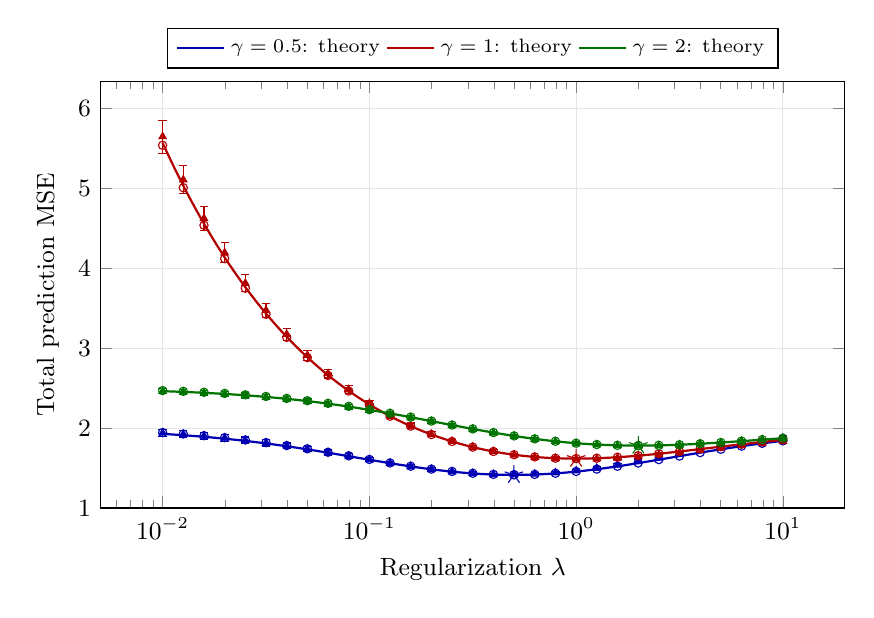
\begin{tikzpicture}
\begin{axis}[width=.91\linewidth,height=7cm,
xlabel={Regularization $\lambda$},ylabel={Total prediction MSE},
grid=major,grid style={gray!20},
legend style={font=\scriptsize,at={(0.5,1.03)},anchor=south,legend columns=3},
tick label style={font=\small},label style={font=\small},
xmode=log,
ymin=1]
\addplot[thick,blue!70!black] coordinates {(0.01,1.9272747) (0.010233718,1.9257329) (0.010472898,1.9241618) (0.010717669,1.9225611) (0.01096816,1.9209303) (0.011224506,1.919269) (0.011486843,1.9175768) (0.011755311,1.9158532) (0.012030053,1.914098) (0.012311217,1.9123107) (0.012598953,1.9104908) (0.012893413,1.9086381) (0.013194755,1.906752) (0.01350314,1.9048323) (0.013818733,1.9028785) (0.014141702,1.9008903) (0.014472219,1.8988672) (0.01481046,1.896809) (0.015156608,1.8947152) (0.015510845,1.8925856) (0.015873361,1.8904196) (0.01624435,1.8882172) (0.01662401,1.8859778) (0.017012543,1.8837012) (0.017410157,1.881387) (0.017817063,1.8790351) (0.01823348,1.876645) (0.018659629,1.8742165) (0.019095738,1.8717493) (0.01954204,1.8692433) (0.019998773,1.866698) (0.02046618,1.8641134) (0.020944511,1.8614892) (0.021434022,1.8588253) (0.021934974,1.8561213) (0.022447634,1.8533773) (0.022972275,1.850593) (0.023509179,1.8477683) (0.024058631,1.8449032) (0.024620924,1.8419974) (0.025196359,1.8390511) (0.025785244,1.836064) (0.026387891,1.8330363) (0.027004624,1.8299678) (0.02763577,1.8268587) (0.028281668,1.823709) (0.028942661,1.8205187) (0.029619103,1.8172879) (0.030311355,1.8140169) (0.031019786,1.8107056) (0.031744774,1.8073544) (0.032486707,1.8039634) (0.033245979,1.8005328) (0.034022998,1.7970629) (0.034818176,1.7935541) (0.03563194,1.7900065) (0.036464722,1.7864207) (0.037316968,1.7827969) (0.038189133,1.7791357) (0.039081682,1.7754373) (0.039995091,1.7717025) (0.040929848,1.7679315) (0.041886452,1.7641251) (0.042865414,1.7602838) (0.043867256,1.7564082) (0.044892513,1.7524989) (0.045941731,1.7485567) (0.047015472,1.7445822) (0.048114308,1.7405763) (0.049238826,1.7365398) (0.050389626,1.7324733) (0.051567322,1.7283779) (0.052772544,1.7242545) (0.054005933,1.7201039) (0.055268149,1.7159271) (0.056559865,1.7117251) (0.05788177,1.707499) (0.059234571,1.7032499) (0.06061899,1.6989788) (0.062035765,1.6946868) (0.063485652,1.6903753) (0.064969426,1.6860453) (0.066487878,1.6816982) (0.06804182,1.6773351) (0.069632079,1.6729574) (0.071259506,1.6685664) (0.072924969,1.6641635) (0.074629357,1.6597501) (0.076373579,1.6553275) (0.078158567,1.6508973) (0.079985273,1.6464609) (0.081854673,1.6420199) (0.083767764,1.6375756) (0.085725567,1.6331298) (0.087729128,1.6286839) (0.089779516,1.6242395) (0.091877824,1.6197983) (0.094025174,1.6153619) (0.096222712,1.6109319) (0.09847161,1.60651) (0.10077307,1.6020979) (0.10312832,1.5976974) (0.10553861,1.59331) (0.10800524,1.5889375) (0.11052951,1.5845816) (0.11311279,1.5802442) (0.11575644,1.5759269) (0.11846187,1.5716315) (0.12123054,1.5673598) (0.12406392,1.5631134) (0.12696351,1.5588943) (0.12993088,1.5547042) (0.1329676,1.5505447) (0.13607529,1.5464178) (0.13925561,1.5423251) (0.14251027,1.5382685) (0.14584099,1.5342496) (0.14924955,1.5302703) (0.15273779,1.5263322) (0.15630754,1.5224371) (0.15996073,1.5185867) (0.1636993,1.5147827) (0.16752525,1.5110268) (0.17144061,1.5073207) (0.17544749,1.503666) (0.17954801,1.5000644) (0.18374437,1.4965175) (0.18803881,1.4930269) (0.19243361,1.4895942) (0.19693113,1.4862209) (0.20153377,1.4829086) (0.20624398,1.4796588) (0.21106427,1.4764729) (0.21599722,1.4733526) (0.22104546,1.470299) (0.22621169,1.4673138) (0.23149867,1.4643982) (0.23690921,1.4615537) (0.2424462,1.4587814) (0.24811261,1.4560827) (0.25391144,1.4534589) (0.25984581,1.4509111) (0.26591887,1.4484406) (0.27213388,1.4460485) (0.27849414,1.4437359) (0.28500304,1.4415039) (0.29166408,1.4393534) (0.29848079,1.4372856) (0.30545682,1.4353014) (0.3125959,1.4334017) (0.31990183,1.4315874) (0.32737851,1.4298593) (0.33502993,1.4282183) (0.34286019,1.4266651) (0.35087345,1.4252004) (0.35907399,1.423825) (0.36746619,1.4225393) (0.37605454,1.4213442) (0.38484361,1.4202401) (0.3938381,1.4192275) (0.4030428,1.4183069) (0.41246264,1.4174788) (0.42210263,1.4167435) (0.43196793,1.4161013) (0.4420638,1.4155527) (0.45239562,1.4150977) (0.46296892,1.4147367) (0.47378934,1.4144698) (0.48486265,1.4142971) (0.49619476,1.4142187) (0.50779172,1.4142347) (0.51965973,1.414345) (0.53180511,1.4145496) (0.54423435,1.4148484) (0.55695409,1.4152413) (0.56997111,1.415728) (0.58329236,1.4163083) (0.59692495,1.4169821) (0.61087616,1.4177489) (0.62515344,1.4186083) (0.6397644,1.4195601) (0.65471684,1.4206038) (0.67001875,1.4217388) (0.68567829,1.4229646) (0.70170383,1.4242807) (0.71810391,1.4256865) (0.73488729,1.4271812) (0.75206293,1.4287642) (0.76963999,1.4304348) (0.78762786,1.4321922) (0.80603614,1.4340355) (0.82487466,1.435964) (0.84415346,1.4379766) (0.86388284,1.4400725) (0.88407334,1.4422506) (0.90473572,1.4445101) (0.92588103,1.4468497) (0.94752053,1.4492685) (0.96966579,1.4517653) (0.99232862,1.454339) (1.0155211,1.4569883) (1.0392557,1.459712) (1.063545,1.4625089) (1.0884019,1.4653777) (1.1138398,1.468317) (1.1398723,1.4713255) (1.1665131,1.4744018) (1.1937766,1.4775446) (1.2216773,1.4807522) (1.2502301,1.4840233) (1.2794503,1.4873565) (1.3093533,1.49075) (1.3399553,1.4942025) (1.3712724,1.4977124) (1.4033215,1.501278) (1.4361197,1.5048978) (1.4696844,1.5085701) (1.5040336,1.5122932) (1.5391855,1.5160656) (1.5751591,1.5198855) (1.6119734,1.5237512) (1.6496481,1.5276611) (1.6882033,1.5316133) (1.7276597,1.5356063) (1.7680382,1.5396381) (1.8093604,1.5437072) (1.8516484,1.5478116) (1.8949248,1.5519498) (1.9392126,1.5561198) (1.9845355,1.56032) (2.0309176,1.5645485) (2.0783838,1.5688036) (2.1269594,1.5730836) (2.1766703,1.5773866) (2.227543,1.5817109) (2.2796046,1.5860547) (2.3328831,1.5904164) (2.3874068,1.5947941) (2.4432048,1.5991862) (2.5003069,1.6035909) (2.5587435,1.6080065) (2.618546,1.6124313) (2.6797461,1.6168636) (2.7423766,1.6213018) (2.8064708,1.6257443) (2.8720631,1.6301894) (2.9391884,1.6346354) (3.0078825,1.6390809) (3.0781821,1.6435243) (3.1501248,1.6479639) (3.2237489,1.6523984) (3.2990937,1.6568261) (3.3761994,1.6612458) (3.4551073,1.6656558) (3.5358594,1.6700548) (3.6184988,1.6744414) (3.7030696,1.6788143) (3.789617,1.6831722) (3.8781871,1.6875136) (3.9688274,1.6918375) (4.061586,1.6961425) (4.1565126,1.7004275) (4.2536577,1.7046913) (4.3530734,1.7089328) (4.4548125,1.7131508) (4.5589295,1.7173444) (4.6654799,1.7215124) (4.7745205,1.725654) (4.8861097,1.729768) (5.0003068,1.7338537) (5.117173,1.7379101) (5.2367705,1.7419364) (5.3591633,1.7459317) (5.4844166,1.7498953) (5.6125973,1.7538265) (5.7437737,1.7577244) (5.8780161,1.7615885) (6.0153959,1.7654181) (6.1559865,1.7692126) (6.299863,1.7729713) (6.4471021,1.7766939) (6.5977825,1.7803797) (6.7519845,1.7840283) (6.9097905,1.7876393) (7.0712848,1.7912122) (7.2365534,1.7947467) (7.4056847,1.7982424) (7.5787689,1.8016989) (7.7558983,1.8051162) (7.9371676,1.8084937) (8.1226735,1.8118315) (8.312515,1.8151291) (8.5067934,1.8183866) (8.7056125,1.8216036) (8.9090783,1.8247802) (9.1172995,1.8279162) (9.3303872,1.8310115) (9.5484551,1.8340662) (9.7716197,1.8370801) (10,1.8400534)};
\addlegendentry{$\gamma=0.5$: theory}
\addplot[only marks,mark=o,mark size=1.5pt,blue!70!black,forget plot] coordinates {(0.01,1.9438032) (0.012589254,1.9260379) (0.015848932,1.9048693) (0.019952623,1.8799495) (0.025118864,1.8510308) (0.031622777,1.8180275) (0.039810717,1.7810822) (0.050118723,1.7406245) (0.063095734,1.6974097) (0.079432823,1.6525246) (0.1,1.6073513) (0.12589254,1.5634896) (0.15848932,1.5226476) (0.19952623,1.4865175) (0.25118864,1.4566522) (0.31622777,1.4343602) (0.39810717,1.4206241) (0.5,1.4160441) (0.50118723,1.4160446) (0.63095734,1.4208091) (0.79432823,1.4346806) (1,1.4570073) (1.2589254,1.4867551) (1.5848932,1.5225666) (1.9952623,1.5628486) (2.5118864,1.6058858) (3.1622777,1.6499693) (3.9810717,1.6935252) (5.0118723,1.7352209) (6.3095734,1.7740361) (7.9432823,1.8092885) (10,1.8406186)};
\addplot[only marks,mark=triangle*,mark size=1.5pt,blue!70!black,forget plot,error bars/.cd,y dir=both,y explicit] coordinates {(0.01,1.9400776) +- (0,0.046661258) (0.012589254,1.9222878) +- (0,0.045450128) (0.015848932,1.9011036) +- (0,0.044039343) (0.019952623,1.8761822) +- (0,0.042420651) (0.025118864,1.847281) +- (0,0.040594601) (0.031622777,1.8143187) +- (0,0.038572508) (0.039810717,1.7774397) +- (0,0.036377387) (0.050118723,1.737072) +- (0,0.034043535) (0.063095734,1.6939669) +- (0,0.031614875) (0.079432823,1.6492064) +- (0,0.029142732) (0.1,1.6041724) +- (0,0.02668408) (0.12589254,1.5604763) +- (0,0.024301143) (0.15848932,1.5198559) +- (0,0.022062429) (0.19952623,1.4840547) +- (0,0.020043905) (0.25118864,1.4546972) +- (0,0.01832769) (0.31622777,1.4331745) +- (0,0.016995078) (0.39810717,1.4205486) +- (0,0.016112427) (0.5,1.4174625) +- (0,0.015715435) (0.50118723,1.4174807) +- (0,0.015713804) (0.63095734,1.4241845) +- (0,0.015790417) (0.79432823,1.4404077) +- (0,0.0162953) (1,1.4654409) +- (0,0.017159896) (1.2589254,1.4981593) +- (0,0.018310663) (1.5848932,1.5370944) +- (0,0.019677906) (1.9952623,1.580538) +- (0,0.021197599) (2.5118864,1.6266685) +- (0,0.022810402) (3.1622777,1.6736898) +- (0,0.024460983) (3.9810717,1.7199636) +- (0,0.026098605) (5.0118723,1.7641172) +- (0,0.027678742) (6.3095734,1.805111) +- (0,0.029164971) (7.9432823,1.8422613) +- (0,0.030530421) (10,1.8752199) +- (0,0.031758304)};
\addplot[only marks,mark=star,mark size=3.5pt,blue!70!black,forget plot] coordinates {(0.5,1.4142136)};
\addplot[thick,red!70!black] coordinates {(0.01,5.5686681) (0.010233718,5.5120392) (0.010472898,5.4560789) (0.010717669,5.4007799) (0.01096816,5.3461347) (0.011224506,5.2921361) (0.011486843,5.2387768) (0.011755311,5.1860497) (0.012030053,5.1339478) (0.012311217,5.0824642) (0.012598953,5.0315919) (0.012893413,4.9813241) (0.013194755,4.9316543) (0.01350314,4.8825756) (0.013818733,4.8340816) (0.014141702,4.7861657) (0.014472219,4.7388217) (0.01481046,4.6920431) (0.015156608,4.6458237) (0.015510845,4.6001574) (0.015873361,4.555038) (0.01624435,4.5104596) (0.01662401,4.4664161) (0.017012543,4.4229017) (0.017410157,4.3799105) (0.017817063,4.3374369) (0.01823348,4.2954751) (0.018659629,4.2540196) (0.019095738,4.2130648) (0.01954204,4.1726052) (0.019998773,4.1326354) (0.02046618,4.0931502) (0.020944511,4.0541441) (0.021434022,4.015612) (0.021934974,3.9775488) (0.022447634,3.9399493) (0.022972275,3.9028085) (0.023509179,3.8661215) (0.024058631,3.8298833) (0.024620924,3.7940892) (0.025196359,3.7587343) (0.025785244,3.7238138) (0.026387891,3.6893232) (0.027004624,3.6552578) (0.02763577,3.6216131) (0.028281668,3.5883844) (0.028942661,3.5555675) (0.029619103,3.5231579) (0.030311355,3.4911512) (0.031019786,3.4595432) (0.031744774,3.4283297) (0.032486707,3.3975064) (0.033245979,3.3670692) (0.034022998,3.3370141) (0.034818176,3.307337) (0.03563194,3.278034) (0.036464722,3.2491011) (0.037316968,3.2205344) (0.038189133,3.1923301) (0.039081682,3.1644844) (0.039995091,3.1369937) (0.040929848,3.1098541) (0.041886452,3.083062) (0.042865414,3.0566139) (0.043867256,3.0305061) (0.044892513,3.0047353) (0.045941731,2.9792979) (0.047015472,2.9541904) (0.048114308,2.9294096) (0.049238826,2.904952) (0.050389626,2.8808144) (0.051567322,2.8569935) (0.052772544,2.8334862) (0.054005933,2.8102892) (0.055268149,2.7873994) (0.056559865,2.7648137) (0.05788177,2.7425291) (0.059234571,2.7205425) (0.06061899,2.6988511) (0.062035765,2.6774517) (0.063485652,2.6563416) (0.064969426,2.6355179) (0.066487878,2.6149778) (0.06804182,2.5947184) (0.069632079,2.5747371) (0.071259506,2.555031) (0.072924969,2.5355975) (0.074629357,2.5164341) (0.076373579,2.4975379) (0.078158567,2.4789066) (0.079985273,2.4605374) (0.081854673,2.442428) (0.083767764,2.4245758) (0.085725567,2.4069784) (0.087729128,2.3896334) (0.089779516,2.3725383) (0.091877824,2.3556909) (0.094025174,2.3390888) (0.096222712,2.3227296) (0.09847161,2.3066112) (0.10077307,2.2907313) (0.10312832,2.2750877) (0.10553861,2.2596783) (0.10800524,2.2445008) (0.11052951,2.2295531) (0.11311279,2.2148332) (0.11575644,2.200339) (0.11846187,2.1860684) (0.12123054,2.1720195) (0.12406392,2.1581903) (0.12696351,2.1445787) (0.12993088,2.1311828) (0.1329676,2.1180008) (0.13607529,2.1050308) (0.13925561,2.0922708) (0.14251027,2.0797191) (0.14584099,2.0673739) (0.14924955,2.0552332) (0.15273779,2.0432955) (0.15630754,2.0315588) (0.15996073,2.0200216) (0.1636993,2.008682) (0.16752525,1.9975384) (0.17144061,1.9865892) (0.17544749,1.9758327) (0.17954801,1.9652673) (0.18374437,1.9548913) (0.18803881,1.9447033) (0.19243361,1.9347015) (0.19693113,1.9248845) (0.20153377,1.9152508) (0.20624398,1.9057988) (0.21106427,1.8965271) (0.21599722,1.8874341) (0.22104546,1.8785185) (0.22621169,1.8697787) (0.23149867,1.8612133) (0.23690921,1.852821) (0.2424462,1.8446003) (0.24811261,1.8365498) (0.25391144,1.8286682) (0.25984581,1.8209541) (0.26591887,1.8134062) (0.27213388,1.8060231) (0.27849414,1.7988035) (0.28500304,1.7917462) (0.29166408,1.7848498) (0.29848079,1.778113) (0.30545682,1.7715345) (0.3125959,1.7651132) (0.31990183,1.7588477) (0.32737851,1.7527369) (0.33502993,1.7467794) (0.34286019,1.740974) (0.35087345,1.7353196) (0.35907399,1.7298149) (0.36746619,1.7244587) (0.37605454,1.7192498) (0.38484361,1.714187) (0.3938381,1.7092692) (0.4030428,1.7044952) (0.41246264,1.6998637) (0.42210263,1.6953737) (0.43196793,1.6910239) (0.4420638,1.6868132) (0.45239562,1.6827404) (0.46296892,1.6788045) (0.47378934,1.6750041) (0.48486265,1.6713382) (0.49619476,1.6678057) (0.50779172,1.6644053) (0.51965973,1.6611359) (0.53180511,1.6579964) (0.54423435,1.6549856) (0.55695409,1.6521024) (0.56997111,1.6493456) (0.58329236,1.646714) (0.59692495,1.6442065) (0.61087616,1.641822) (0.62515344,1.6395593) (0.6397644,1.6374171) (0.65471684,1.6353944) (0.67001875,1.63349) (0.68567829,1.6317026) (0.70170383,1.6300311) (0.71810391,1.6284743) (0.73488729,1.6270311) (0.75206293,1.6257001) (0.76963999,1.6244802) (0.78762786,1.6233702) (0.80603614,1.6223688) (0.82487466,1.6214749) (0.84415346,1.6206871) (0.86388284,1.6200042) (0.88407334,1.619425) (0.90473572,1.6189482) (0.92588103,1.6185725) (0.94752053,1.6182967) (0.96966579,1.6181194) (0.99232862,1.6180393) (1.0155211,1.6180551) (1.0392557,1.6181656) (1.063545,1.6183693) (1.0884019,1.6186649) (1.1138398,1.619051) (1.1398723,1.6195264) (1.1665131,1.6200895) (1.1937766,1.6207391) (1.2216773,1.6214737) (1.2502301,1.6222919) (1.2794503,1.6231923) (1.3093533,1.6241735) (1.3399553,1.625234) (1.3712724,1.6263724) (1.4033215,1.6275872) (1.4361197,1.6288769) (1.4696844,1.6302401) (1.5040336,1.6316752) (1.5391855,1.6331808) (1.5751591,1.6347554) (1.6119734,1.6363974) (1.6496481,1.6381054) (1.6882033,1.6398777) (1.7276597,1.6417129) (1.7680382,1.6436093) (1.8093604,1.6455656) (1.8516484,1.6475799) (1.8949248,1.6496509) (1.9392126,1.651777) (1.9845355,1.6539565) (2.0309176,1.6561879) (2.0783838,1.6584696) (2.1269594,1.6608001) (2.1766703,1.6631777) (2.227543,1.6656008) (2.2796046,1.6680679) (2.3328831,1.6705773) (2.3874068,1.6731276) (2.4432048,1.675717) (2.5003069,1.678344) (2.5587435,1.6810071) (2.618546,1.6837046) (2.6797461,1.686435) (2.7423766,1.6891968) (2.8064708,1.6919883) (2.8720631,1.6948079) (2.9391884,1.6976543) (3.0078825,1.7005258) (3.0781821,1.7034208) (3.1501248,1.706338) (3.2237489,1.7092757) (3.2990937,1.7122325) (3.3761994,1.715207) (3.4551073,1.7181975) (3.5358594,1.7212028) (3.6184988,1.7242213) (3.7030696,1.7272517) (3.789617,1.7302925) (3.8781871,1.7333424) (3.9688274,1.7363999) (4.061586,1.7394638) (4.1565126,1.7425328) (4.2536577,1.7456054) (4.3530734,1.7486805) (4.4548125,1.7517568) (4.5589295,1.754833) (4.6654799,1.757908) (4.7745205,1.7609804) (4.8861097,1.7640493) (5.0003068,1.7671133) (5.117173,1.7701715) (5.2367705,1.7732227) (5.3591633,1.7762658) (5.4844166,1.7792998) (5.6125973,1.7823237) (5.7437737,1.7853366) (5.8780161,1.7883374) (6.0153959,1.7913252) (6.1559865,1.7942992) (6.299863,1.7972583) (6.4471021,1.8002019) (6.5977825,1.8031291) (6.7519845,1.8060391) (6.9097905,1.8089311) (7.0712848,1.8118044) (7.2365534,1.8146583) (7.4056847,1.8174921) (7.5787689,1.8203052) (7.7558983,1.8230969) (7.9371676,1.8258667) (8.1226735,1.828614) (8.312515,1.8313383) (8.5067934,1.8340389) (8.7056125,1.8367156) (8.9090783,1.8393677) (9.1172995,1.8419949) (9.3303872,1.8445968) (9.5484551,1.847173) (9.7716197,1.8497231) (10,1.8522468)};
\addlegendentry{$\gamma=1$: theory}
\addplot[only marks,mark=o,mark size=1.5pt,red!70!black,forget plot] coordinates {(0.01,5.5387084) (0.012589254,5.0080684) (0.015848932,4.53734) (0.019952623,4.1200881) (0.025118864,3.7506054) (0.031622777,3.4238562) (0.039810717,3.1354218) (0.050118723,2.8814404) (0.063095734,2.6585422) (0.079432823,2.4637859) (0.1,2.2946) (0.12589254,2.1487306) (0.15848932,2.0241977) (0.19952623,1.9192556) (0.25118864,1.8323555) (0.31622777,1.762109) (0.39810717,1.7072502) (0.50118723,1.6665955) (0.63095734,1.6390017) (0.79432823,1.6233237) (1,1.6183735) (1.2589254,1.6228869) (1.5848932,1.6355027) (1.9952623,1.654761) (2.5118864,1.6791269) (3.1622777,1.7070392) (3.9810717,1.7369794) (5.0118723,1.7675504) (6.3095734,1.7975498) (7.9432823,1.8260227) (10,1.8522864)};
\addplot[only marks,mark=triangle*,mark size=1.5pt,red!70!black,forget plot,error bars/.cd,y dir=both,y explicit] coordinates {(0.01,5.6477536) +- (0,0.20626495) (0.012589254,5.1070607) +- (0,0.17571123) (0.015848932,4.6242364) +- (0,0.14889631) (0.019952623,4.1939977) +- (0,0.12560077) (0.025118864,3.8116742) +- (0,0.10565827) (0.031622777,3.4730382) +- (0,0.088867615) (0.039810717,3.1741821) +- (0,0.074954373) (0.050118723,2.9114564) +- (0,0.063575907) (0.063095734,2.6814603) +- (0,0.054353827) (0.079432823,2.4810633) +- (0,0.046914316) (0.1,2.3074334) +- (0,0.040920846) (0.12589254,2.1580507) +- (0,0.036092072) (0.15848932,2.0307007) +- (0,0.032205429) (0.19952623,1.9234475) +- (0,0.029091172) (0.25118864,1.8345953) +- (0,0.026622124) (0.31622777,1.7626443) +- (0,0.024702892) (0.39810717,1.7062469) +- (0,0.023260372) (0.50118723,1.6641622) +- (0,0.022235932) (0.63095734,1.6352121) +- (0,0.021579238) (0.79432823,1.6182346) +- (0,0.021243816) (1,1.6120387) +- (0,0.021184564) (1.2589254,1.6153653) +- (0,0.021357128) (1.5848932,1.6268611) +- (0,0.021718585) (1.9952623,1.6450731) +- (0,0.02222856) (2.5118864,1.6684702) +- (0,0.022850029) (3.1622777,1.6954919) +- (0,0.023549458) (3.9810717,1.724618) +- (0,0.024296439) (5.0118723,1.7544493) +- (0,0.025063296) (6.3095734,1.783781) +- (0,0.025825099) (7.9432823,1.8116561) +- (0,0.026560185) (10,1.83739) +- (0,0.027250961)};
\addplot[only marks,mark=star,mark size=3.5pt,red!70!black,forget plot] coordinates {(1,1.618034)};
\addplot[thick,green!45!black] coordinates {(0.01,2.4618106) (0.010233718,2.4609593) (0.010472898,2.4600899) (0.010717669,2.4592021) (0.01096816,2.4582956) (0.011224506,2.4573701) (0.011486843,2.4564251) (0.011755311,2.4554603) (0.012030053,2.4544754) (0.012311217,2.4534699) (0.012598953,2.4524436) (0.012893413,2.4513959) (0.013194755,2.4503267) (0.01350314,2.4492354) (0.013818733,2.4481216) (0.014141702,2.4469851) (0.014472219,2.4458253) (0.01481046,2.444642) (0.015156608,2.4434346) (0.015510845,2.4422028) (0.015873361,2.4409462) (0.01624435,2.4396643) (0.01662401,2.4383568) (0.017012543,2.4370232) (0.017410157,2.4356631) (0.017817063,2.4342761) (0.01823348,2.4328617) (0.018659629,2.4314195) (0.019095738,2.4299492) (0.01954204,2.4284501) (0.019998773,2.426922) (0.02046618,2.4253644) (0.020944511,2.4237768) (0.021434022,2.4221588) (0.021934974,2.42051) (0.022447634,2.4188299) (0.022972275,2.4171181) (0.023509179,2.4153742) (0.024058631,2.4135977) (0.024620924,2.4117881) (0.025196359,2.4099451) (0.025785244,2.4080682) (0.026387891,2.406157) (0.027004624,2.404211) (0.02763577,2.4022299) (0.028281668,2.4002132) (0.028942661,2.3981604) (0.029619103,2.3960712) (0.030311355,2.3939452) (0.031019786,2.391782) (0.031744774,2.3895811) (0.032486707,2.3873422) (0.033245979,2.3850648) (0.034022998,2.3827487) (0.034818176,2.3803934) (0.03563194,2.3779986) (0.036464722,2.3755639) (0.037316968,2.373089) (0.038189133,2.3705736) (0.039081682,2.3680173) (0.039995091,2.3654198) (0.040929848,2.3627808) (0.041886452,2.3601) (0.042865414,2.3573772) (0.043867256,2.3546121) (0.044892513,2.3518045) (0.045941731,2.3489541) (0.047015472,2.3460607) (0.048114308,2.3431241) (0.049238826,2.3401441) (0.050389626,2.3371206) (0.051567322,2.3340534) (0.052772544,2.3309425) (0.054005933,2.3277876) (0.055268149,2.3245888) (0.056559865,2.3213459) (0.05788177,2.3180589) (0.059234571,2.3147278) (0.06061899,2.3113526) (0.062035765,2.3079333) (0.063485652,2.3044699) (0.064969426,2.3009626) (0.066487878,2.2974115) (0.06804182,2.2938166) (0.069632079,2.2901782) (0.071259506,2.2864963) (0.072924969,2.2827713) (0.074629357,2.2790033) (0.076373579,2.2751927) (0.078158567,2.2713396) (0.079985273,2.2674445) (0.081854673,2.2635077) (0.083767764,2.2595295) (0.085725567,2.2555104) (0.087729128,2.2514509) (0.089779516,2.2473513) (0.091877824,2.2432123) (0.094025174,2.2390343) (0.096222712,2.2348179) (0.09847161,2.2305638) (0.10077307,2.2262725) (0.10312832,2.2219447) (0.10553861,2.2175812) (0.10800524,2.2131826) (0.11052951,2.2087497) (0.11311279,2.2042833) (0.11575644,2.1997842) (0.11846187,2.1952533) (0.12123054,2.1906915) (0.12406392,2.1860997) (0.12696351,2.1814788) (0.12993088,2.1768298) (0.1329676,2.1721537) (0.13607529,2.1674516) (0.13925561,2.1627245) (0.14251027,2.1579736) (0.14584099,2.1531999) (0.14924955,2.1484045) (0.15273779,2.1435888) (0.15630754,2.1387538) (0.15996073,2.1339007) (0.1636993,2.129031) (0.16752525,2.1241457) (0.17144061,2.1192462) (0.17544749,2.1143339) (0.17954801,2.10941) (0.18374437,2.1044759) (0.18803881,2.099533) (0.19243361,2.0945826) (0.19693113,2.0896263) (0.20153377,2.0846653) (0.20624398,2.0797012) (0.21106427,2.0747354) (0.21599722,2.0697693) (0.22104546,2.0648044) (0.22621169,2.0598423) (0.23149867,2.0548843) (0.23690921,2.0499321) (0.2424462,2.044987) (0.24811261,2.0400506) (0.25391144,2.0351245) (0.25984581,2.03021) (0.26591887,2.0253089) (0.27213388,2.0204224) (0.27849414,2.0155523) (0.28500304,2.0106999) (0.29166408,2.0058668) (0.29848079,2.0010546) (0.30545682,1.9962646) (0.3125959,1.9914984) (0.31990183,1.9867575) (0.32737851,1.9820433) (0.33502993,1.9773573) (0.34286019,1.9727009) (0.35087345,1.9680757) (0.35907399,1.9634829) (0.36746619,1.9589241) (0.37605454,1.9544006) (0.38484361,1.9499138) (0.3938381,1.945465) (0.4030428,1.9410557) (0.41246264,1.936687) (0.42210263,1.9323604) (0.43196793,1.928077) (0.4420638,1.9238382) (0.45239562,1.9196452) (0.46296892,1.9154992) (0.47378934,1.9114014) (0.48486265,1.9073529) (0.49619476,1.903355) (0.50779172,1.8994086) (0.51965973,1.8955149) (0.53180511,1.8916749) (0.54423435,1.8878897) (0.55695409,1.8841602) (0.56997111,1.8804875) (0.58329236,1.8768725) (0.59692495,1.8733161) (0.61087616,1.8698191) (0.62515344,1.8663824) (0.6397644,1.8630069) (0.65471684,1.8596934) (0.67001875,1.8564425) (0.68567829,1.853255) (0.70170383,1.8501316) (0.71810391,1.847073) (0.73488729,1.8440798) (0.75206293,1.8411526) (0.76963999,1.8382919) (0.78762786,1.8354983) (0.80603614,1.8327723) (0.82487466,1.8301143) (0.84415346,1.8275248) (0.86388284,1.8250042) (0.88407334,1.8225528) (0.90473572,1.820171) (0.92588103,1.817859) (0.94752053,1.8156172) (0.96966579,1.8134457) (0.99232862,1.8113448) (1.0155211,1.8093146) (1.0392557,1.8073552) (1.063545,1.8054667) (1.0884019,1.8036493) (1.1138398,1.8019029) (1.1398723,1.8002276) (1.1665131,1.7986233) (1.1937766,1.7970899) (1.2216773,1.7956273) (1.2502301,1.7942355) (1.2794503,1.7929142) (1.3093533,1.7916633) (1.3399553,1.7904825) (1.3712724,1.7893716) (1.4033215,1.7883303) (1.4361197,1.7873583) (1.4696844,1.7864553) (1.5040336,1.7856208) (1.5391855,1.7848545) (1.5751591,1.7841559) (1.6119734,1.7835245) (1.6496481,1.78296) (1.6882033,1.7824617) (1.7276597,1.7820291) (1.7680382,1.7816617) (1.8093604,1.7813588) (1.8516484,1.7811199) (1.8949248,1.7809442) (1.9392126,1.7808311) (1.9845355,1.7807798) (2.0309176,1.7807898) (2.0783838,1.7808602) (2.1269594,1.7809902) (2.1766703,1.781179) (2.227543,1.7814259) (2.2796046,1.78173) (2.3328831,1.7820904) (2.3874068,1.7825063) (2.4432048,1.7829768) (2.5003069,1.7835009) (2.5587435,1.7840776) (2.618546,1.7847062) (2.6797461,1.7853855) (2.7423766,1.7861146) (2.8064708,1.7868926) (2.8720631,1.7877183) (2.9391884,1.7885907) (3.0078825,1.7895089) (3.0781821,1.7904717) (3.1501248,1.791478) (3.2237489,1.7925269) (3.2990937,1.7936173) (3.3761994,1.7947479) (3.4551073,1.7959178) (3.5358594,1.7971257) (3.6184988,1.7983707) (3.7030696,1.7996515) (3.789617,1.8009671) (3.8781871,1.8023162) (3.9688274,1.8036979) (4.061586,1.8051108) (4.1565126,1.8065539) (4.2536577,1.8080261) (4.3530734,1.8095262) (4.4548125,1.8110531) (4.5589295,1.8126056) (4.6654799,1.8141826) (4.7745205,1.815783) (4.8861097,1.8174056) (5.0003068,1.8190494) (5.117173,1.8207131) (5.2367705,1.8223958) (5.3591633,1.8240963) (5.4844166,1.8258134) (5.6125973,1.8275463) (5.7437737,1.8292937) (5.8780161,1.8310545) (6.0153959,1.8328279) (6.1559865,1.8346127) (6.299863,1.8364079) (6.4471021,1.8382124) (6.5977825,1.8400254) (6.7519845,1.8418457) (6.9097905,1.8436726) (7.0712848,1.8455049) (7.2365534,1.8473418) (7.4056847,1.8491823) (7.5787689,1.8510256) (7.7558983,1.8528707) (7.9371676,1.8547168) (8.1226735,1.8565632) (8.312515,1.8584088) (8.5067934,1.860253) (8.7056125,1.8620949) (8.9090783,1.8639338) (9.1172995,1.8657689) (9.3303872,1.8675995) (9.5484551,1.8694249) (9.7716197,1.8712444) (10,1.8730573)};
\addlegendentry{$\gamma=2$: theory}
\addplot[only marks,mark=o,mark size=1.5pt,green!45!black,forget plot] coordinates {(0.01,2.4694416) (0.012589254,2.4598558) (0.015848932,2.4481053) (0.019952623,2.4337924) (0.025118864,2.4164918) (0.031622777,2.395772) (0.039810717,2.3712291) (0.050118723,2.3425319) (0.063095734,2.3094792) (0.079432823,2.272062) (0.1,2.2305226) (0.12589254,2.1853969) (0.15848932,2.1375282) (0.19952623,2.0880416) (0.25118864,2.0382799) (0.31622777,1.9897069) (0.39810717,1.9437948) (0.50118723,1.9019141) (0.63095734,1.8652397) (0.79432823,1.8346834) (1,1.8108527) (1.2589254,1.7940336) (1.5848932,1.7841924) (1.9952623,1.7809921) (2,1.7809918) (2.5118864,1.7838233) (3.1622777,1.7918487) (3.9810717,1.8040639) (5.0118723,1.8193704) (6.3095734,1.8366575) (7.9432823,1.8548824) (10,1.8731378)};
\addplot[only marks,mark=triangle*,mark size=1.5pt,green!45!black,forget plot,error bars/.cd,y dir=both,y explicit] coordinates {(0.01,2.4605476) +- (0,0.033143343) (0.012589254,2.4510524) +- (0,0.032792661) (0.015848932,2.4394142) +- (0,0.032370095) (0.019952623,2.4252398) +- (0,0.031866118) (0.025118864,2.408109) +- (0,0.031272442) (0.031622777,2.3875955) +- (0,0.030583349) (0.039810717,2.3633005) +- (0,0.029797279) (0.050118723,2.3348969) +- (0,0.028918455) (0.063095734,2.3021852) +- (0,0.027958186) (0.079432823,2.2651546) +- (0,0.026935363) (0.1,2.22404) +- (0,0.025875752) (0.12589254,2.1793635) +- (0,0.024809928) (0.15848932,2.1319477) +- (0,0.023770164) (0.19952623,2.082892) +- (0,0.022787025) (0.25118864,2.0335119) +- (0,0.021886517) (0.31622777,1.985248) +- (0,0.021088381) (0.39810717,1.9395594) +- (0,0.020405584) (0.50118723,1.8978175) +- (0,0.019844674) (0.63095734,1.8612142) +- (0,0.019406601) (0.79432823,1.8306909) +- (0,0.019087742) (1,1.8068922) +- (0,0.018881007) (1.2589254,1.7901409) +- (0,0.018776906) (1.5848932,1.7804333) +- (0,0.018764484) (1.9952623,1.7774511) +- (0,0.018832001) (2,1.7774535) +- (0,0.01883307) (2.5118864,1.7805905) +- (0,0.018967338) (3.1622777,1.7890086) +- (0,0.019158206) (3.9810717,1.8016858) +- (0,0.019392251) (5.0118723,1.8175033) +- (0,0.019657182) (6.3095734,1.8353282) +- (0,0.019941002) (7.9432823,1.8540958) +- (0,0.020232363) (10,1.8728798) +- (0,0.020521017)};
\addplot[only marks,mark=star,mark size=3.5pt,green!45!black,forget plot] coordinates {(2,1.7807764)};
\end{axis}
\end{tikzpicture}
\caption{固定 $\gamma$ 扫描 $\lambda$。实线为渐近风险，空心圆为条件风险均值，实心三角为独立测试 MSE 均值；误差线为均值的近似点态 $95\%$ 区间。星号标出理论最优点 $\lambda^*=\gamma/\alpha^2$。}
\label{fig:lambda}
\end{figure}
固定正则的维数扫描见图~\ref{fig:gamma}。较弱正则在插值阈值附近产生明显风险峰，峰值位置可以偏离 $\gamma=1$；增强正则后，噪声放大得到缓和，曲线更平滑。该比较保持样本量、总信号强度和噪声方差一致，反映固定收缩强度对不同维数的适应程度。
\begin{figure}[htbp]
\centering
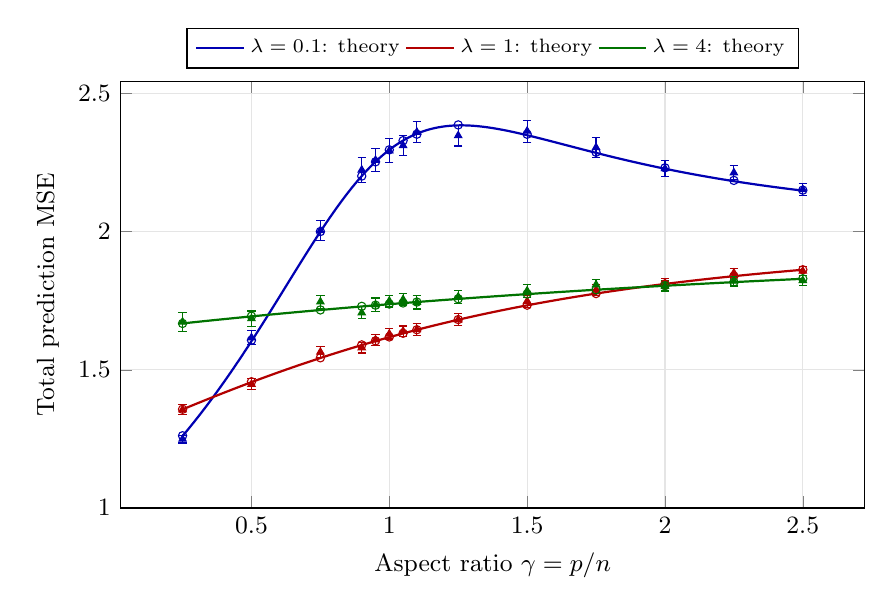
\begin{tikzpicture}
\begin{axis}[width=.91\linewidth,height=7cm,
xlabel={Aspect ratio $\gamma=p/n$},ylabel={Total prediction MSE},
grid=major,grid style={gray!20},
legend style={font=\scriptsize,at={(0.5,1.03)},anchor=south,legend columns=3},
tick label style={font=\small},label style={font=\small},
% linear x axis
ymin=1]
\addplot[thick,blue!70!black] coordinates {(0.25,1.2604032) (0.25752508,1.2693693) (0.26505017,1.2784217) (0.27257525,1.2875608) (0.28010033,1.2967865) (0.28762542,1.3060993) (0.2951505,1.3154992) (0.30267559,1.3249862) (0.31020067,1.3345604) (0.31772575,1.3442219) (0.32525084,1.3539705) (0.33277592,1.3638061) (0.340301,1.3737285) (0.34782609,1.3837374) (0.35535117,1.3938326) (0.36287625,1.4040136) (0.37040134,1.41428) (0.37792642,1.4246311) (0.38545151,1.4350665) (0.39297659,1.4455854) (0.40050167,1.4561869) (0.40802676,1.4668703) (0.41555184,1.4776345) (0.42307692,1.4884784) (0.43060201,1.4994009) (0.43812709,1.5104007) (0.44565217,1.5214763) (0.45317726,1.5326264) (0.46070234,1.5438493) (0.46822742,1.5551432) (0.47575251,1.5665064) (0.48327759,1.5779367) (0.49080268,1.5894322) (0.49832776,1.6009906) (0.50585284,1.6126095) (0.51337793,1.6242865) (0.52090301,1.6360189) (0.52842809,1.6478039) (0.53595318,1.6596386) (0.54347826,1.6715199) (0.55100334,1.6834447) (0.55852843,1.6954096) (0.56605351,1.7074112) (0.5735786,1.7194456) (0.58110368,1.7315093) (0.58862876,1.7435982) (0.59615385,1.7557083) (0.60367893,1.7678354) (0.61120401,1.779975) (0.6187291,1.7921228) (0.62625418,1.804274) (0.63377926,1.8164239) (0.64130435,1.8285675) (0.64882943,1.8407) (0.65635452,1.852816) (0.6638796,1.8649104) (0.67140468,1.8769778) (0.67892977,1.8890128) (0.68645485,1.9010097) (0.69397993,1.9129629) (0.70150502,1.9248667) (0.7090301,1.9367153) (0.71655518,1.9485029) (0.72408027,1.9602236) (0.73160535,1.9718714) (0.73913043,1.9834404) (0.74665552,1.9949247) (0.7541806,2.0063182) (0.76170569,2.017615) (0.76923077,2.0288091) (0.77675585,2.0398948) (0.78428094,2.0508661) (0.79180602,2.0617173) (0.7993311,2.0724426) (0.80685619,2.0830365) (0.81438127,2.0934934) (0.82190635,2.103808) (0.82943144,2.1139751) (0.83695652,2.1239895) (0.84448161,2.1338463) (0.85200669,2.1435407) (0.85953177,2.1530681) (0.86705686,2.1624242) (0.87458194,2.1716047) (0.88210702,2.1806056) (0.88963211,2.1894233) (0.89715719,2.1980541) (0.90468227,2.2064949) (0.91220736,2.2147425) (0.91973244,2.2227943) (0.92725753,2.2306476) (0.93478261,2.2383003) (0.94230769,2.2457502) (0.94983278,2.2529959) (0.95735786,2.2600357) (0.96488294,2.2668684) (0.97240803,2.2734933) (0.97993311,2.2799096) (0.98745819,2.286117) (0.99498328,2.2921154) (1.0025084,2.2979049) (1.0100334,2.3034859) (1.0175585,2.3088591) (1.0250836,2.3140253) (1.0326087,2.3189858) (1.0401338,2.3237418) (1.0476589,2.3282949) (1.0551839,2.3326469) (1.062709,2.3367999) (1.0702341,2.3407559) (1.0777592,2.3445174) (1.0852843,2.3480869) (1.0928094,2.351467) (1.1003344,2.3546606) (1.1078595,2.3576708) (1.1153846,2.3605005) (1.1229097,2.3631531) (1.1304348,2.3656319) (1.1379599,2.3679403) (1.1454849,2.3700818) (1.15301,2.37206) (1.1605351,2.3738787) (1.1680602,2.3755415) (1.1755853,2.3770522) (1.1831104,2.3784146) (1.1906355,2.3796326) (1.1981605,2.38071) (1.2056856,2.3816506) (1.2132107,2.3824584) (1.2207358,2.3831373) (1.2282609,2.3836911) (1.235786,2.3841236) (1.243311,2.3844387) (1.2508361,2.3846402) (1.2583612,2.3847319) (1.2658863,2.3847174) (1.2734114,2.3846005) (1.2809365,2.3843849) (1.2884615,2.384074) (1.2959866,2.3836715) (1.3035117,2.3831808) (1.3110368,2.3826053) (1.3185619,2.3819484) (1.326087,2.3812134) (1.333612,2.3804035) (1.3411371,2.3795218) (1.3486622,2.3785715) (1.3561873,2.3775555) (1.3637124,2.3764768) (1.3712375,2.3753382) (1.3787625,2.3741426) (1.3862876,2.3728926) (1.3938127,2.371591) (1.4013378,2.3702402) (1.4088629,2.3688428) (1.416388,2.3674012) (1.423913,2.3659177) (1.4314381,2.3643946) (1.4389632,2.3628342) (1.4464883,2.3612386) (1.4540134,2.3596099) (1.4615385,2.35795) (1.4690635,2.3562608) (1.4765886,2.3545444) (1.4841137,2.3528024) (1.4916388,2.3510366) (1.4991639,2.3492487) (1.506689,2.3474403) (1.514214,2.3456129) (1.5217391,2.3437681) (1.5292642,2.3419073) (1.5367893,2.3400319) (1.5443144,2.3381432) (1.5518395,2.3362426) (1.5593645,2.3343312) (1.5668896,2.3324102) (1.5744147,2.3304807) (1.5819398,2.3285439) (1.5894649,2.3266008) (1.59699,2.3246524) (1.6045151,2.3226996) (1.6120401,2.3207433) (1.6195652,2.3187845) (1.6270903,2.3168239) (1.6346154,2.3148624) (1.6421405,2.3129008) (1.6496656,2.3109396) (1.6571906,2.3089797) (1.6647157,2.3070217) (1.6722408,2.3050662) (1.6797659,2.3031138) (1.687291,2.3011651) (1.6948161,2.2992207) (1.7023411,2.297281) (1.7098662,2.2953465) (1.7173913,2.2934177) (1.7249164,2.2914951) (1.7324415,2.289579) (1.7399666,2.2876698) (1.7474916,2.285768) (1.7550167,2.2838738) (1.7625418,2.2819875) (1.7700669,2.2801096) (1.777592,2.2782403) (1.7851171,2.2763798) (1.7926421,2.2745284) (1.8001672,2.2726864) (1.8076923,2.270854) (1.8152174,2.2690314) (1.8227425,2.2672188) (1.8302676,2.2654163) (1.8377926,2.2636242) (1.8453177,2.2618426) (1.8528428,2.2600716) (1.8603679,2.2583115) (1.867893,2.2565622) (1.8754181,2.2548239) (1.8829431,2.2530967) (1.8904682,2.2513808) (1.8979933,2.2496761) (1.9055184,2.2479827) (1.9130435,2.2463008) (1.9205686,2.2446304) (1.9280936,2.2429715) (1.9356187,2.2413242) (1.9431438,2.2396885) (1.9506689,2.2380645) (1.958194,2.2364521) (1.9657191,2.2348513) (1.9732441,2.2332623) (1.9807692,2.2316849) (1.9882943,2.2301193) (1.9958194,2.2285653) (2.0033445,2.227023) (2.0108696,2.2254923) (2.0183946,2.2239734) (2.0259197,2.222466) (2.0334448,2.2209702) (2.0409699,2.219486) (2.048495,2.2180133) (2.0560201,2.2165522) (2.0635452,2.2151024) (2.0710702,2.2136641) (2.0785953,2.2122372) (2.0861204,2.2108216) (2.0936455,2.2094173) (2.1011706,2.2080242) (2.1086957,2.2066422) (2.1162207,2.2052714) (2.1237458,2.2039116) (2.1312709,2.2025629) (2.138796,2.201225) (2.1463211,2.1998981) (2.1538462,2.1985819) (2.1613712,2.1972765) (2.1688963,2.1959817) (2.1764214,2.1946976) (2.1839465,2.193424) (2.1914716,2.1921609) (2.1989967,2.1909082) (2.2065217,2.1896658) (2.2140468,2.1884336) (2.2215719,2.1872117) (2.229097,2.1859998) (2.2366221,2.184798) (2.2441472,2.1836062) (2.2516722,2.1824242) (2.2591973,2.1812521) (2.2667224,2.1800897) (2.2742475,2.1789369) (2.2817726,2.1777937) (2.2892977,2.1766601) (2.2968227,2.1755359) (2.3043478,2.174421) (2.3118729,2.1733154) (2.319398,2.172219) (2.3269231,2.1711318) (2.3344482,2.1700536) (2.3419732,2.1689844) (2.3494983,2.1679241) (2.3570234,2.1668726) (2.3645485,2.1658298) (2.3720736,2.1647958) (2.3795987,2.1637703) (2.3871237,2.1627534) (2.3946488,2.1617449) (2.4021739,2.1607448) (2.409699,2.159753) (2.4172241,2.1587694) (2.4247492,2.157794) (2.4322742,2.1568267) (2.4397993,2.1558673) (2.4473244,2.154916) (2.4548495,2.1539724) (2.4623746,2.1530367) (2.4698997,2.1521087) (2.4774247,2.1511884) (2.4849498,2.1502756) (2.4924749,2.1493704) (2.5,2.1484726)};
\addlegendentry{$\lambda=0.1$: theory}
\addplot[only marks,mark=o,mark size=1.5pt,blue!70!black,forget plot] coordinates {(0.25,1.2613073) (0.5,1.6072894) (0.75,2.0003572) (0.9,2.2010644) (0.95,2.2527092) (1,2.2960176) (1.05,2.3294074) (1.1,2.3526713) (1.25,2.3862655) (1.5,2.3524195) (1.75,2.2872398) (2,2.2309333) (2.25,2.1854314) (2.5,2.1502524)};
\addplot[only marks,mark=triangle*,mark size=1.5pt,blue!70!black,forget plot,error bars/.cd,y dir=both,y explicit] coordinates {(0.25,1.2492451) +- (0,0.014178011) (0.5,1.6162578) +- (0,0.025338404) (0.75,2.0037775) +- (0,0.036849124) (0.9,2.2232146) +- (0,0.044376455) (0.95,2.2587469) +- (0,0.042621149) (1,2.2930233) +- (0,0.043891985) (1.05,2.3115946) +- (0,0.036408028) (1.1,2.3600823) +- (0,0.039005585) (1.25,2.3476263) +- (0,0.037827907) (1.5,2.3638873) +- (0,0.039780592) (1.75,2.3045975) +- (0,0.035061379) (2,2.2283443) +- (0,0.027644937) (2.25,2.2131531) +- (0,0.024838111) (2.5,2.1524982) +- (0,0.022821477)};
\addplot[thick,red!70!black] coordinates {(0.25,1.35666) (0.25752508,1.3597633) (0.26505017,1.362859) (0.27257525,1.3659471) (0.28010033,1.3690274) (0.28762542,1.3720999) (0.2951505,1.3751645) (0.30267559,1.378221) (0.31020067,1.3812693) (0.31772575,1.3843095) (0.32525084,1.3873413) (0.33277592,1.3903647) (0.340301,1.3933797) (0.34782609,1.396386) (0.35535117,1.3993837) (0.36287625,1.4023726) (0.37040134,1.4053527) (0.37792642,1.4083239) (0.38545151,1.4112861) (0.39297659,1.4142392) (0.40050167,1.4171831) (0.40802676,1.4201178) (0.41555184,1.4230433) (0.42307692,1.4259593) (0.43060201,1.4288659) (0.43812709,1.431763) (0.44565217,1.4346504) (0.45317726,1.4375283) (0.46070234,1.4403964) (0.46822742,1.4432547) (0.47575251,1.4461031) (0.48327759,1.4489417) (0.49080268,1.4517702) (0.49832776,1.4545888) (0.50585284,1.4573972) (0.51337793,1.4601955) (0.52090301,1.4629836) (0.52842809,1.4657614) (0.53595318,1.468529) (0.54347826,1.4712861) (0.55100334,1.4740329) (0.55852843,1.4767692) (0.56605351,1.479495) (0.5735786,1.4822103) (0.58110368,1.4849149) (0.58862876,1.487609) (0.59615385,1.4902923) (0.60367893,1.492965) (0.61120401,1.4956269) (0.6187291,1.498278) (0.62625418,1.5009183) (0.63377926,1.5035477) (0.64130435,1.5061662) (0.64882943,1.5087738) (0.65635452,1.5113705) (0.6638796,1.5139562) (0.67140468,1.5165309) (0.67892977,1.5190945) (0.68645485,1.5216471) (0.69397993,1.5241886) (0.70150502,1.526719) (0.7090301,1.5292383) (0.71655518,1.5317465) (0.72408027,1.5342434) (0.73160535,1.5367293) (0.73913043,1.5392039) (0.74665552,1.5416673) (0.7541806,1.5441195) (0.76170569,1.5465604) (0.76923077,1.5489901) (0.77675585,1.5514086) (0.78428094,1.5538158) (0.79180602,1.5562117) (0.7993311,1.5585964) (0.80685619,1.5609697) (0.81438127,1.5633318) (0.82190635,1.5656826) (0.82943144,1.5680221) (0.83695652,1.5703504) (0.84448161,1.5726673) (0.85200669,1.5749729) (0.85953177,1.5772673) (0.86705686,1.5795504) (0.87458194,1.5818222) (0.88210702,1.5840827) (0.88963211,1.586332) (0.89715719,1.58857) (0.90468227,1.5907968) (0.91220736,1.5930123) (0.91973244,1.5952166) (0.92725753,1.5974097) (0.93478261,1.5995916) (0.94230769,1.6017622) (0.94983278,1.6039218) (0.95735786,1.6060701) (0.96488294,1.6082073) (0.97240803,1.6103334) (0.97993311,1.6124483) (0.98745819,1.6145522) (0.99498328,1.6166449) (1.0025084,1.6187267) (1.0100334,1.6207974) (1.0175585,1.622857) (1.0250836,1.6249057) (1.0326087,1.6269434) (1.0401338,1.6289702) (1.0476589,1.630986) (1.0551839,1.632991) (1.062709,1.634985) (1.0702341,1.6369683) (1.0777592,1.6389407) (1.0852843,1.6409023) (1.0928094,1.6428531) (1.1003344,1.6447932) (1.1078595,1.6467226) (1.1153846,1.6486414) (1.1229097,1.6505494) (1.1304348,1.6524469) (1.1379599,1.6543338) (1.1454849,1.6562101) (1.15301,1.6580759) (1.1605351,1.6599313) (1.1680602,1.6617761) (1.1755853,1.6636106) (1.1831104,1.6654347) (1.1906355,1.6672484) (1.1981605,1.6690518) (1.2056856,1.6708449) (1.2132107,1.6726278) (1.2207358,1.6744004) (1.2282609,1.6761629) (1.235786,1.6779153) (1.243311,1.6796576) (1.2508361,1.6813898) (1.2583612,1.683112) (1.2658863,1.6848242) (1.2734114,1.6865265) (1.2809365,1.6882189) (1.2884615,1.6899014) (1.2959866,1.6915741) (1.3035117,1.693237) (1.3110368,1.6948902) (1.3185619,1.6965336) (1.326087,1.6981674) (1.333612,1.6997916) (1.3411371,1.7014062) (1.3486622,1.7030113) (1.3561873,1.7046069) (1.3637124,1.706193) (1.3712375,1.7077697) (1.3787625,1.7093371) (1.3862876,1.7108951) (1.3938127,1.7124438) (1.4013378,1.7139833) (1.4088629,1.7155136) (1.416388,1.7170348) (1.423913,1.7185468) (1.4314381,1.7200498) (1.4389632,1.7215437) (1.4464883,1.7230287) (1.4540134,1.7245047) (1.4615385,1.7259719) (1.4690635,1.7274302) (1.4765886,1.7288796) (1.4841137,1.7303204) (1.4916388,1.7317524) (1.4991639,1.7331757) (1.506689,1.7345904) (1.514214,1.7359966) (1.5217391,1.7373941) (1.5292642,1.7387832) (1.5367893,1.7401639) (1.5443144,1.7415361) (1.5518395,1.7429) (1.5593645,1.7442556) (1.5668896,1.7456028) (1.5744147,1.7469419) (1.5819398,1.7482728) (1.5894649,1.7495955) (1.59699,1.7509102) (1.6045151,1.7522167) (1.6120401,1.7535153) (1.6195652,1.7548059) (1.6270903,1.7560886) (1.6346154,1.7573635) (1.6421405,1.7586305) (1.6496656,1.7598897) (1.6571906,1.7611411) (1.6647157,1.7623849) (1.6722408,1.763621) (1.6797659,1.7648495) (1.687291,1.7660704) (1.6948161,1.7672839) (1.7023411,1.7684898) (1.7098662,1.7696883) (1.7173913,1.7708794) (1.7249164,1.7720631) (1.7324415,1.7732396) (1.7399666,1.7744087) (1.7474916,1.7755707) (1.7550167,1.7767255) (1.7625418,1.7778731) (1.7700669,1.7790136) (1.777592,1.7801471) (1.7851171,1.7812736) (1.7926421,1.7823931) (1.8001672,1.7835057) (1.8076923,1.7846114) (1.8152174,1.7857103) (1.8227425,1.7868024) (1.8302676,1.7878877) (1.8377926,1.7889663) (1.8453177,1.7900382) (1.8528428,1.7911035) (1.8603679,1.7921622) (1.867893,1.7932143) (1.8754181,1.7942599) (1.8829431,1.7952991) (1.8904682,1.7963318) (1.8979933,1.7973581) (1.9055184,1.7983781) (1.9130435,1.7993918) (1.9205686,1.8003992) (1.9280936,1.8014003) (1.9356187,1.8023953) (1.9431438,1.8033841) (1.9506689,1.8043668) (1.958194,1.8053434) (1.9657191,1.806314) (1.9732441,1.8072786) (1.9807692,1.8082372) (1.9882943,1.8091899) (1.9958194,1.8101367) (2.0033445,1.8110777) (2.0108696,1.8120128) (2.0183946,1.8129422) (2.0259197,1.8138658) (2.0334448,1.8147838) (2.0409699,1.815696) (2.048495,1.8166027) (2.0560201,1.8175038) (2.0635452,1.8183993) (2.0710702,1.8192893) (2.0785953,1.8201738) (2.0861204,1.8210529) (2.0936455,1.8219265) (2.1011706,1.8227948) (2.1086957,1.8236578) (2.1162207,1.8245154) (2.1237458,1.8253678) (2.1312709,1.8262149) (2.138796,1.8270569) (2.1463211,1.8278936) (2.1538462,1.8287253) (2.1613712,1.8295518) (2.1688963,1.8303733) (2.1764214,1.8311897) (2.1839465,1.8320012) (2.1914716,1.8328077) (2.1989967,1.8336092) (2.2065217,1.8344059) (2.2140468,1.8351977) (2.2215719,1.8359846) (2.229097,1.8367668) (2.2366221,1.8375441) (2.2441472,1.8383168) (2.2516722,1.8390847) (2.2591973,1.839848) (2.2667224,1.8406066) (2.2742475,1.8413606) (2.2817726,1.84211) (2.2892977,1.8428549) (2.2968227,1.8435952) (2.3043478,1.8443311) (2.3118729,1.8450624) (2.319398,1.8457894) (2.3269231,1.846512) (2.3344482,1.8472301) (2.3419732,1.847944) (2.3494983,1.8486535) (2.3570234,1.8493588) (2.3645485,1.8500598) (2.3720736,1.8507565) (2.3795987,1.8514491) (2.3871237,1.8521375) (2.3946488,1.8528217) (2.4021739,1.8535019) (2.409699,1.8541779) (2.4172241,1.8548499) (2.4247492,1.8555179) (2.4322742,1.8561818) (2.4397993,1.8568418) (2.4473244,1.8574978) (2.4548495,1.8581499) (2.4623746,1.8587981) (2.4698997,1.8594424) (2.4774247,1.8600829) (2.4849498,1.8607196) (2.4924749,1.8613525) (2.5,1.8619816)};
\addlegendentry{$\lambda=1$: theory}
\addplot[only marks,mark=o,mark size=1.5pt,red!70!black,forget plot] coordinates {(0.25,1.3571889) (0.5,1.4568289) (0.75,1.5434999) (0.9,1.5901915) (0.95,1.6048353) (1,1.6189551) (1.05,1.632244) (1.1,1.6449559) (1.25,1.6818533) (1.5,1.7339042) (1.75,1.7760079) (2,1.8109359) (2.25,1.8391822) (2.5,1.8621922)};
\addplot[only marks,mark=triangle*,mark size=1.5pt,red!70!black,forget plot,error bars/.cd,y dir=both,y explicit] coordinates {(0.25,1.3558944) +- (0,0.01901679) (0.5,1.4478099) +- (0,0.019718349) (0.75,1.5642405) +- (0,0.019218414) (0.9,1.5802251) +- (0,0.019425027) (0.95,1.6087559) +- (0,0.020499274) (1,1.6299493) +- (0,0.018427986) (1.05,1.639841) +- (0,0.018695682) (1.1,1.6456823) +- (0,0.02241068) (1.25,1.6815848) +- (0,0.020976128) (1.5,1.7484845) +- (0,0.021844704) (1.75,1.7890077) +- (0,0.018887) (2,1.8122951) +- (0,0.018320544) (2.25,1.8502697) +- (0,0.017702501) (2.5,1.8574461) +- (0,0.017307168)};
\addplot[thick,green!45!black] coordinates {(0.25,1.6678919) (0.25752508,1.6686919) (0.26505017,1.6694897) (0.27257525,1.6702852) (0.28010033,1.6710785) (0.28762542,1.6718696) (0.2951505,1.6726584) (0.30267559,1.673445) (0.31020067,1.6742295) (0.31772575,1.6750116) (0.32525084,1.6757916) (0.33277592,1.6765694) (0.340301,1.677345) (0.34782609,1.6781184) (0.35535117,1.6788897) (0.36287625,1.6796587) (0.37040134,1.6804256) (0.37792642,1.6811903) (0.38545151,1.6819529) (0.39297659,1.6827133) (0.40050167,1.6834715) (0.40802676,1.6842276) (0.41555184,1.6849816) (0.42307692,1.6857334) (0.43060201,1.6864831) (0.43812709,1.6872307) (0.44565217,1.6879761) (0.45317726,1.6887195) (0.46070234,1.6894607) (0.46822742,1.6901998) (0.47575251,1.6909369) (0.48327759,1.6916718) (0.49080268,1.6924047) (0.49832776,1.6931354) (0.50585284,1.6938642) (0.51337793,1.6945908) (0.52090301,1.6953154) (0.52842809,1.6960379) (0.53595318,1.6967583) (0.54347826,1.6974767) (0.55100334,1.6981931) (0.55852843,1.6989074) (0.56605351,1.6996197) (0.5735786,1.70033) (0.58110368,1.7010383) (0.58862876,1.7017445) (0.59615385,1.7024487) (0.60367893,1.703151) (0.61120401,1.7038512) (0.6187291,1.7045494) (0.62625418,1.7052456) (0.63377926,1.7059399) (0.64130435,1.7066322) (0.64882943,1.7073225) (0.65635452,1.7080108) (0.6638796,1.7086972) (0.67140468,1.7093816) (0.67892977,1.7100641) (0.68645485,1.7107446) (0.69397993,1.7114232) (0.70150502,1.7120998) (0.7090301,1.7127745) (0.71655518,1.7134473) (0.72408027,1.7141182) (0.73160535,1.7147871) (0.73913043,1.7154541) (0.74665552,1.7161193) (0.7541806,1.7167825) (0.76170569,1.7174439) (0.76923077,1.7181033) (0.77675585,1.7187609) (0.78428094,1.7194166) (0.79180602,1.7200704) (0.7993311,1.7207223) (0.80685619,1.7213724) (0.81438127,1.7220207) (0.82190635,1.722667) (0.82943144,1.7233116) (0.83695652,1.7239543) (0.84448161,1.7245951) (0.85200669,1.7252341) (0.85953177,1.7258713) (0.86705686,1.7265067) (0.87458194,1.7271403) (0.88210702,1.727772) (0.88963211,1.7284019) (0.89715719,1.7290301) (0.90468227,1.7296564) (0.91220736,1.730281) (0.91973244,1.7309038) (0.92725753,1.7315247) (0.93478261,1.732144) (0.94230769,1.7327614) (0.94983278,1.7333771) (0.95735786,1.733991) (0.96488294,1.7346032) (0.97240803,1.7352136) (0.97993311,1.7358222) (0.98745819,1.7364292) (0.99498328,1.7370344) (1.0025084,1.7376378) (1.0100334,1.7382396) (1.0175585,1.7388396) (1.0250836,1.7394379) (1.0326087,1.7400345) (1.0401338,1.7406294) (1.0476589,1.7412226) (1.0551839,1.7418141) (1.062709,1.7424039) (1.0702341,1.742992) (1.0777592,1.7435784) (1.0852843,1.7441632) (1.0928094,1.7447463) (1.1003344,1.7453277) (1.1078595,1.7459075) (1.1153846,1.7464856) (1.1229097,1.747062) (1.1304348,1.7476368) (1.1379599,1.74821) (1.1454849,1.7487815) (1.15301,1.7493514) (1.1605351,1.7499197) (1.1680602,1.7504864) (1.1755853,1.7510514) (1.1831104,1.7516148) (1.1906355,1.7521767) (1.1981605,1.7527369) (1.2056856,1.7532955) (1.2132107,1.7538525) (1.2207358,1.7544079) (1.2282609,1.7549618) (1.235786,1.755514) (1.243311,1.7560647) (1.2508361,1.7566139) (1.2583612,1.7571614) (1.2658863,1.7577074) (1.2734114,1.7582519) (1.2809365,1.7587948) (1.2884615,1.7593361) (1.2959866,1.7598759) (1.3035117,1.7604142) (1.3110368,1.7609509) (1.3185619,1.7614861) (1.326087,1.7620198) (1.333612,1.7625519) (1.3411371,1.7630826) (1.3486622,1.7636117) (1.3561873,1.7641394) (1.3637124,1.7646655) (1.3712375,1.7651901) (1.3787625,1.7657133) (1.3862876,1.7662349) (1.3938127,1.7667551) (1.4013378,1.7672738) (1.4088629,1.767791) (1.416388,1.7683067) (1.423913,1.768821) (1.4314381,1.7693339) (1.4389632,1.7698452) (1.4464883,1.7703551) (1.4540134,1.7708636) (1.4615385,1.7713706) (1.4690635,1.7718762) (1.4765886,1.7723804) (1.4841137,1.7728831) (1.4916388,1.7733844) (1.4991639,1.7738843) (1.506689,1.7743827) (1.514214,1.7748798) (1.5217391,1.7753754) (1.5292642,1.7758697) (1.5367893,1.7763625) (1.5443144,1.7768539) (1.5518395,1.777344) (1.5593645,1.7778327) (1.5668896,1.7783199) (1.5744147,1.7788058) (1.5819398,1.7792904) (1.5894649,1.7797735) (1.59699,1.7802553) (1.6045151,1.7807358) (1.6120401,1.7812148) (1.6195652,1.7816926) (1.6270903,1.7821689) (1.6346154,1.782644) (1.6421405,1.7831177) (1.6496656,1.78359) (1.6571906,1.784061) (1.6647157,1.7845307) (1.6722408,1.7849991) (1.6797659,1.7854662) (1.687291,1.7859319) (1.6948161,1.7863963) (1.7023411,1.7868594) (1.7098662,1.7873212) (1.7173913,1.7877817) (1.7249164,1.788241) (1.7324415,1.7886989) (1.7399666,1.7891555) (1.7474916,1.7896109) (1.7550167,1.7900649) (1.7625418,1.7905177) (1.7700669,1.7909693) (1.777592,1.7914195) (1.7851171,1.7918685) (1.7926421,1.7923162) (1.8001672,1.7927627) (1.8076923,1.7932079) (1.8152174,1.7936519) (1.8227425,1.7940946) (1.8302676,1.7945361) (1.8377926,1.7949764) (1.8453177,1.7954154) (1.8528428,1.7958532) (1.8603679,1.7962898) (1.867893,1.7967251) (1.8754181,1.7971592) (1.8829431,1.7975922) (1.8904682,1.7980239) (1.8979933,1.7984544) (1.9055184,1.7988836) (1.9130435,1.7993117) (1.9205686,1.7997386) (1.9280936,1.8001644) (1.9356187,1.8005889) (1.9431438,1.8010122) (1.9506689,1.8014344) (1.958194,1.8018554) (1.9657191,1.8022752) (1.9732441,1.8026938) (1.9807692,1.8031113) (1.9882943,1.8035276) (1.9958194,1.8039428) (2.0033445,1.8043568) (2.0108696,1.8047696) (2.0183946,1.8051813) (2.0259197,1.8055919) (2.0334448,1.8060013) (2.0409699,1.8064096) (2.048495,1.8068167) (2.0560201,1.8072227) (2.0635452,1.8076276) (2.0710702,1.8080314) (2.0785953,1.808434) (2.0861204,1.8088356) (2.0936455,1.809236) (2.1011706,1.8096353) (2.1086957,1.8100335) (2.1162207,1.8104306) (2.1237458,1.8108266) (2.1312709,1.8112216) (2.138796,1.8116154) (2.1463211,1.8120081) (2.1538462,1.8123998) (2.1613712,1.8127903) (2.1688963,1.8131798) (2.1764214,1.8135683) (2.1839465,1.8139556) (2.1914716,1.8143419) (2.1989967,1.8147271) (2.2065217,1.8151113) (2.2140468,1.8154944) (2.2215719,1.8158764) (2.229097,1.8162574) (2.2366221,1.8166374) (2.2441472,1.8170163) (2.2516722,1.8173941) (2.2591973,1.8177709) (2.2667224,1.8181467) (2.2742475,1.8185215) (2.2817726,1.8188952) (2.2892977,1.8192679) (2.2968227,1.8196396) (2.3043478,1.8200103) (2.3118729,1.8203799) (2.319398,1.8207486) (2.3269231,1.8211162) (2.3344482,1.8214828) (2.3419732,1.8218484) (2.3494983,1.8222131) (2.3570234,1.8225767) (2.3645485,1.8229393) (2.3720736,1.823301) (2.3795987,1.8236616) (2.3871237,1.8240213) (2.3946488,1.82438) (2.4021739,1.8247377) (2.409699,1.8250945) (2.4172241,1.8254502) (2.4247492,1.825805) (2.4322742,1.8261589) (2.4397993,1.8265117) (2.4473244,1.8268637) (2.4548495,1.8272146) (2.4623746,1.8275646) (2.4698997,1.8279137) (2.4774247,1.8282618) (2.4849498,1.828609) (2.4924749,1.8289552) (2.5,1.8293005)};
\addlegendentry{$\lambda=4$: theory}
\addplot[only marks,mark=o,mark size=1.5pt,green!45!black,forget plot] coordinates {(0.25,1.6677714) (0.5,1.6940856) (0.75,1.7167603) (0.9,1.7297184) (0.95,1.7338709) (1,1.7380901) (1.05,1.741854) (1.1,1.7452617) (1.25,1.7569672) (1.5,1.7744193) (1.75,1.7897901) (2,1.8044258) (2.25,1.8175566) (2.5,1.8294786)};
\addplot[only marks,mark=triangle*,mark size=1.5pt,green!45!black,forget plot,error bars/.cd,y dir=both,y explicit] coordinates {(0.25,1.6733038) +- (0,0.033791701) (0.5,1.6855279) +- (0,0.027351263) (0.75,1.7460876) +- (0,0.023771055) (0.9,1.7064366) +- (0,0.022088039) (0.95,1.7352145) +- (0,0.02452488) (1,1.7489281) +- (0,0.021536671) (1.05,1.7545493) +- (0,0.020187443) (1.1,1.7442704) +- (0,0.02427699) (1.25,1.7642389) +- (0,0.022902277) (1.5,1.7857254) +- (0,0.022579886) (1.75,1.80805) +- (0,0.018657854) (2,1.8031395) +- (0,0.018092399) (2.25,1.8209717) +- (0,0.017678138) (2.5,1.8233153) +- (0,0.016928761)};
\end{axis}
\end{tikzpicture}
\caption{固定 $\lambda$ 扫描 $\gamma$。实线为渐近风险，空心圆为条件风险均值，实心三角为独立测试 MSE 均值；误差线为均值的近似点态 $95\%$ 区间。}
\label{fig:gamma}
\end{figure}
图~\ref{fig:biasvariance}~用式~\eqref{eq:asymbv}~解释上述现象：随着 $\lambda$ 增加，收缩偏差上升，训练噪声方差下降，总风险在两者平衡处达到最低点。不可约噪声贡献始终为 $1$。该图由解析公式计算，用于说明风险变化的机制。
\begin{figure}[htbp]\centering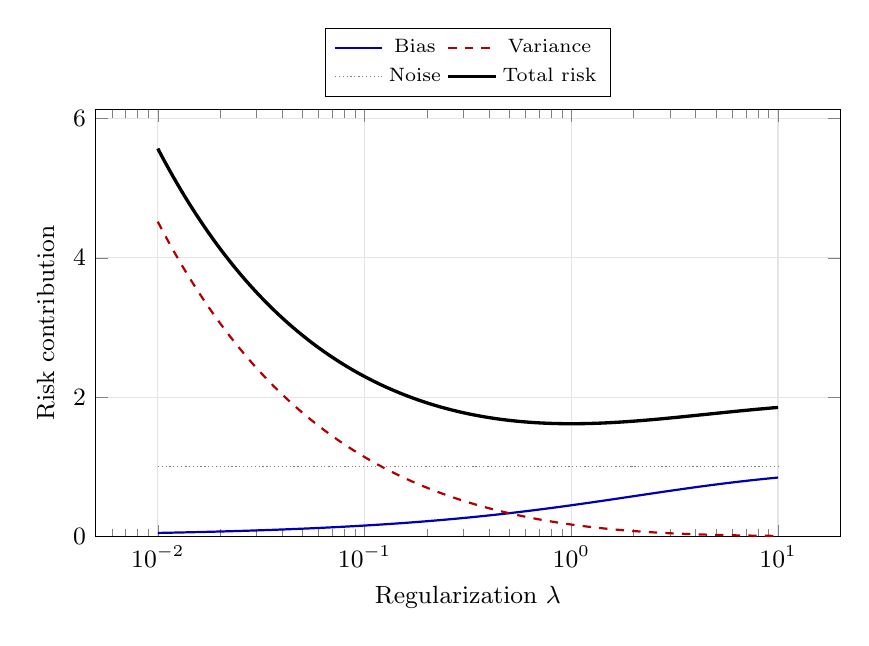
\begin{tikzpicture}
\begin{axis}[width=.91\linewidth,height=7cm,xmode=log,ymin=0,
xlabel={Regularization $\lambda$},ylabel={Risk contribution},grid=major,grid style={gray!20},
legend style={font=\scriptsize,at={(.5,1.03)},anchor=south,legend columns=2},
tick label style={font=\small},label style={font=\small}]
\addplot[blue!70!black,thick] coordinates {(0.01,0.049937617) (0.010353218,0.05080967) (0.010718913,0.051696872) (0.011097525,0.05259948) (0.01148951,0.053517759) (0.011895341,0.054451976) (0.012315506,0.055402402) (0.012750512,0.056369313) (0.013200884,0.057352989) (0.013667164,0.058353716) (0.014149913,0.059371783) (0.014649714,0.060407483) (0.015167169,0.061461117) (0.015702901,0.062532985) (0.016257557,0.063623398) (0.016831804,0.064732667) (0.017426334,0.065861111) (0.018041864,0.067009052) (0.018679136,0.068176818) (0.019338918,0.069364741) (0.020022004,0.070573158) (0.020729218,0.071802414) (0.021461412,0.073052855) (0.022219469,0.074324835) (0.023004301,0.075618712) (0.023816856,0.076934849) (0.024658111,0.078273617) (0.025529081,0.079635389) (0.026430815,0.081020544) (0.0273644,0.082429469) (0.028330961,0.083862553) (0.029331663,0.085320194) (0.030367711,0.086802792) (0.031440355,0.088310755) (0.032550886,0.089844496) (0.033700643,0.091404434) (0.034891012,0.092990992) (0.036123427,0.0946046) (0.037399373,0.096245693) (0.038720388,0.097914713) (0.040088063,0.099612106) (0.041504048,0.10133832) (0.042970047,0.10309382) (0.044487828,0.10487907) (0.04605922,0.10669453) (0.047686117,0.10854069) (0.049370479,0.11041801) (0.051114335,0.11232699) (0.052919787,0.11426811) (0.054789012,0.11624187) (0.056724261,0.11824878) (0.058727866,0.12028934) (0.060802243,0.12236406) (0.06294989,0.12447346) (0.065173396,0.12661806) (0.067475441,0.12879838) (0.069858797,0.13101496) (0.072326339,0.13326833) (0.074881039,0.13555903) (0.077525975,0.13788761) (0.080264335,0.14025461) (0.083099419,0.14266059) (0.086034644,0.1451061) (0.089073546,0.14759169) (0.092219788,0.15011794) (0.095477161,0.15268539) (0.09884959,0.15529463) (0.10234114,0.15794622) (0.10595602,0.16064073) (0.10969858,0.16337873) (0.11357334,0.1661608) (0.11758496,0.16898751) (0.12173827,0.17185943) (0.12603829,0.17477714) (0.1304902,0.17774122) (0.13509935,0.18075223) (0.13987131,0.18381075) (0.14481182,0.18691734) (0.14992684,0.19007258) (0.15522254,0.19327703) (0.16070528,0.19653124) (0.16638169,0.19983577) (0.1722586,0.20319118) (0.17834309,0.20659799) (0.18464249,0.21005675) (0.19116441,0.21356799) (0.19791669,0.21713223) (0.20490747,0.22074998) (0.21214518,0.22442174) (0.21963854,0.22814799) (0.22739658,0.23192922) (0.23542864,0.23576589) (0.24374442,0.23965844) (0.25235392,0.24360731) (0.26126752,0.24761293) (0.27049597,0.25167568) (0.28005039,0.25579594) (0.28994229,0.25997408) (0.30018358,0.26421044) (0.31078662,0.26850532) (0.32176418,0.27285902) (0.33312948,0.2772718) (0.34489623,0.2817439) (0.3570786,0.28627552) (0.36969127,0.29086685) (0.38274945,0.29551802) (0.39626886,0.30022915) (0.41026581,0.30500031) (0.42475716,0.30983154) (0.43976036,0.31472285) (0.45529351,0.31967419) (0.47137531,0.32468547) (0.48802516,0.32975658) (0.50526311,0.33488733) (0.52310993,0.34007751) (0.54158714,0.34532685) (0.56071699,0.35063503) (0.58052255,0.35600167) (0.60102768,0.36142635) (0.62225708,0.36690859) (0.64423635,0.37244784) (0.66699197,0.3780435) (0.69055135,0.38369491) (0.7149429,0.38940136) (0.740196,0.39516204) (0.76634109,0.40097611) (0.79340967,0.40684265) (0.82143436,0.41276066) (0.85044893,0.41872911) (0.88048836,0.42474685) (0.91158883,0.4308127) (0.94378783,0.43692538) (0.97712415,0.44308356) (1,0.4472136) (1.011638,0.44928583) (1.0473709,0.45553069) (1.084366,0.4618166) (1.1226678,0.46814192) (1.1623225,0.47450495) (1.2033778,0.48090393) (1.2458834,0.48733699) (1.2898903,0.49380223) (1.3354516,0.50029767) (1.3826222,0.50682124) (1.4314589,0.51337084) (1.4820207,0.51994427) (1.5343684,0.5265393) (1.5885651,0.53315361) (1.6446762,0.53978484) (1.7027692,0.54643058) (1.7629141,0.55308834) (1.8251835,0.55975562) (1.8896523,0.56642984) (1.9563983,0.5731084) (2.0255019,0.57978866) (2.0970464,0.58646793) (2.1711179,0.59314351) (2.2478058,0.59981267) (2.3272025,0.60647265) (2.4094036,0.61312068) (2.4945081,0.61975399) (2.5826188,0.62636978) (2.6738416,0.63296528) (2.7682866,0.63953771) (2.8660676,0.64608429) (2.9673024,0.65260226) (3.072113,0.6590889) (3.1806257,0.66554149) (3.2929713,0.67195737) (3.4092851,0.67833388) (3.5297073,0.68466842) (3.6543831,0.69095846) (3.7834626,0.69720148) (3.9171015,0.70339505) (4.0554607,0.70953677) (4.1987071,0.71562434) (4.3470132,0.7216555) (4.5005577,0.72762809) (4.6595257,0.73354) (4.8241087,0.73938923) (4.9945051,0.74517383) (5.1709202,0.75089197) (5.3535667,0.7565419) (5.5426645,0.76212195) (5.7384416,0.76763055) (5.941134,0.77306624) (6.1509858,0.77842765) (6.3682499,0.78371349) (6.5931883,0.78892259) (6.8260718,0.79405388) (7.0671813,0.79910639) (7.3168071,0.80407923) (7.5752503,0.80897164) (7.8428221,0.81378294) (8.119845,0.81851254) (8.4066529,0.82315997) (8.7035914,0.82772484) (9.0110183,0.83220686) (9.329304,0.83660583) (9.6588322,0.84092164) (10,0.84515425)};
\addlegendentry{Bias}
\addplot[red!70!black,thick,dashed] coordinates {(0.01,4.5187305) (0.010353218,4.4330256) (0.010718913,4.3488068) (0.011097525,4.2660485) (0.01148951,4.184726) (0.011895341,4.1048146) (0.012315506,4.0262903) (0.012750512,3.9491295) (0.013200884,3.873309) (0.013667164,3.7988057) (0.014149913,3.7255974) (0.014649714,3.653662) (0.015167169,3.5829777) (0.015702901,3.5135233) (0.016257557,3.4452779) (0.016831804,3.3782208) (0.017426334,3.312332) (0.018041864,3.2475915) (0.018679136,3.1839798) (0.019338918,3.1214778) (0.020022004,3.0600666) (0.020729218,2.9997277) (0.021461412,2.940443) (0.022219469,2.8821945) (0.023004301,2.8249647) (0.023816856,2.7687364) (0.024658111,2.7134926) (0.025529081,2.6592167) (0.026430815,2.6058923) (0.0273644,2.5535033) (0.028330961,2.5020339) (0.029331663,2.4514687) (0.030367711,2.4017924) (0.031440355,2.35299) (0.032550886,2.3050467) (0.033700643,2.2579482) (0.034891012,2.2116802) (0.036123427,2.1662288) (0.037399373,2.1215802) (0.038720388,2.0777211) (0.040088063,2.0346381) (0.041504048,1.9923183) (0.042970047,1.950749) (0.044487828,1.9099174) (0.04605922,1.8698115) (0.047686117,1.8304189) (0.049370479,1.7917279) (0.051114335,1.7537268) (0.052919787,1.7164041) (0.054789012,1.6797484) (0.056724261,1.6437489) (0.058727866,1.6083945) (0.060802243,1.5736746) (0.06294989,1.5395787) (0.065173396,1.5060965) (0.067475441,1.4732178) (0.069858797,1.4409328) (0.072326339,1.4092316) (0.074881039,1.3781047) (0.077525975,1.3475427) (0.080264335,1.3175362) (0.083099419,1.2880762) (0.086034644,1.2591538) (0.089073546,1.2307602) (0.092219788,1.2028868) (0.095477161,1.1755251) (0.09884959,1.1486668) (0.10234114,1.1223038) (0.10595602,1.096428) (0.10969858,1.0710316) (0.11357334,1.0461069) (0.11758496,1.0216462) (0.12173827,0.99764211) (0.12603829,0.9740873) (0.1304902,0.95097457) (0.13509935,0.92829687) (0.13987131,0.90604726) (0.14481182,0.88421892) (0.14992684,0.86280515) (0.15522254,0.8417994) (0.16070528,0.82119519) (0.16638169,0.8009862) (0.1722586,0.78116619) (0.17834309,0.76172903) (0.18464249,0.74266873) (0.19116441,0.72397938) (0.19791669,0.70565518) (0.20490747,0.68769043) (0.21214518,0.67007953) (0.21963854,0.65281698) (0.22739658,0.63589738) (0.23542864,0.61931541) (0.24374442,0.60306586) (0.25235392,0.58714359) (0.26126752,0.57154357) (0.27049597,0.55626084) (0.28005039,0.54129053) (0.28994229,0.52662784) (0.30018358,0.51226807) (0.31078662,0.49820658) (0.32176418,0.48443882) (0.33312948,0.47096031) (0.34489623,0.45776664) (0.3570786,0.44485347) (0.36969127,0.43221653) (0.38274945,0.41985161) (0.39626886,0.40775459) (0.41026581,0.39592138) (0.42475716,0.38434797) (0.43976036,0.37303041) (0.45529351,0.3619648) (0.47137531,0.35114731) (0.48802516,0.34057414) (0.50526311,0.33024157) (0.52310993,0.32014591) (0.54158714,0.31028353) (0.56071699,0.30065085) (0.58052255,0.29124431) (0.60102768,0.28206044) (0.62225708,0.27309577) (0.64423635,0.2643469) (0.66699197,0.25581044) (0.69055135,0.24748306) (0.7149429,0.23936146) (0.740196,0.23144237) (0.76634109,0.22372257) (0.79340967,0.21619885) (0.82143436,0.20886804) (0.85044893,0.20172699) (0.88048836,0.19477259) (0.91158883,0.18800176) (0.94378783,0.18141143) (0.97712415,0.17499855) (1,0.17082039) (1.011638,0.16876011) (1.0473709,0.16269312) (1.084366,0.15679459) (1.1226678,0.15106157) (1.1623225,0.14549113) (1.2033778,0.14008034) (1.2458834,0.13482629) (1.2898903,0.12972611) (1.3354516,0.12477693) (1.3826222,0.11997587) (1.4314589,0.11532012) (1.4820207,0.11080683) (1.5343684,0.10643319) (1.5885651,0.10219642) (1.6446762,0.09809371) (1.7027692,0.094122305) (1.7629141,0.090279443) (1.8251835,0.086562381) (1.8896523,0.082968388) (1.9563983,0.079494749) (2.0255019,0.076138765) (2.0970464,0.07289775) (2.1711179,0.069769035) (2.2478058,0.066749965) (2.3272025,0.063837906) (2.4094036,0.061030239) (2.4945081,0.058324365) (2.5826188,0.055717701) (2.6738416,0.05320769) (2.7682866,0.050791791) (2.8660676,0.048467489) (2.9673024,0.04623229) (3.072113,0.044083726) (3.1806257,0.042019353) (3.2929713,0.040036755) (3.4092851,0.038133543) (3.5297073,0.036307357) (3.6543831,0.034555867) (3.7834626,0.032876774) (3.9171015,0.031267813) (4.0554607,0.029726749) (4.1987071,0.028251385) (4.3470132,0.026839558) (4.5005577,0.02548914) (4.6595257,0.024198043) (4.8241087,0.022964216) (4.9945051,0.021785647) (5.1709202,0.020660365) (5.3535667,0.019586439) (5.5426645,0.01856198) (5.7384416,0.017585139) (5.941134,0.016654113) (6.1509858,0.015767139) (6.3682499,0.014922499) (6.5931883,0.014118518) (6.8260718,0.013353566) (7.0671813,0.012626054) (7.3168071,0.011934441) (7.5752503,0.011277229) (7.8428221,0.010652962) (8.119845,0.01006023) (8.4066529,0.0094976669) (8.7035914,0.0089639483) (9.0110183,0.0084577943) (9.329304,0.0079779671) (9.6588322,0.0075232712) (10,0.0070925528)};
\addlegendentry{Variance}
\addplot[black!50,densely dotted] coordinates {(0.01,1) (0.010353218,1) (0.010718913,1) (0.011097525,1) (0.01148951,1) (0.011895341,1) (0.012315506,1) (0.012750512,1) (0.013200884,1) (0.013667164,1) (0.014149913,1) (0.014649714,1) (0.015167169,1) (0.015702901,1) (0.016257557,1) (0.016831804,1) (0.017426334,1) (0.018041864,1) (0.018679136,1) (0.019338918,1) (0.020022004,1) (0.020729218,1) (0.021461412,1) (0.022219469,1) (0.023004301,1) (0.023816856,1) (0.024658111,1) (0.025529081,1) (0.026430815,1) (0.0273644,1) (0.028330961,1) (0.029331663,1) (0.030367711,1) (0.031440355,1) (0.032550886,1) (0.033700643,1) (0.034891012,1) (0.036123427,1) (0.037399373,1) (0.038720388,1) (0.040088063,1) (0.041504048,1) (0.042970047,1) (0.044487828,1) (0.04605922,1) (0.047686117,1) (0.049370479,1) (0.051114335,1) (0.052919787,1) (0.054789012,1) (0.056724261,1) (0.058727866,1) (0.060802243,1) (0.06294989,1) (0.065173396,1) (0.067475441,1) (0.069858797,1) (0.072326339,1) (0.074881039,1) (0.077525975,1) (0.080264335,1) (0.083099419,1) (0.086034644,1) (0.089073546,1) (0.092219788,1) (0.095477161,1) (0.09884959,1) (0.10234114,1) (0.10595602,1) (0.10969858,1) (0.11357334,1) (0.11758496,1) (0.12173827,1) (0.12603829,1) (0.1304902,1) (0.13509935,1) (0.13987131,1) (0.14481182,1) (0.14992684,1) (0.15522254,1) (0.16070528,1) (0.16638169,1) (0.1722586,1) (0.17834309,1) (0.18464249,1) (0.19116441,1) (0.19791669,1) (0.20490747,1) (0.21214518,1) (0.21963854,1) (0.22739658,1) (0.23542864,1) (0.24374442,1) (0.25235392,1) (0.26126752,1) (0.27049597,1) (0.28005039,1) (0.28994229,1) (0.30018358,1) (0.31078662,1) (0.32176418,1) (0.33312948,1) (0.34489623,1) (0.3570786,1) (0.36969127,1) (0.38274945,1) (0.39626886,1) (0.41026581,1) (0.42475716,1) (0.43976036,1) (0.45529351,1) (0.47137531,1) (0.48802516,1) (0.50526311,1) (0.52310993,1) (0.54158714,1) (0.56071699,1) (0.58052255,1) (0.60102768,1) (0.62225708,1) (0.64423635,1) (0.66699197,1) (0.69055135,1) (0.7149429,1) (0.740196,1) (0.76634109,1) (0.79340967,1) (0.82143436,1) (0.85044893,1) (0.88048836,1) (0.91158883,1) (0.94378783,1) (0.97712415,1) (1,1) (1.011638,1) (1.0473709,1) (1.084366,1) (1.1226678,1) (1.1623225,1) (1.2033778,1) (1.2458834,1) (1.2898903,1) (1.3354516,1) (1.3826222,1) (1.4314589,1) (1.4820207,1) (1.5343684,1) (1.5885651,1) (1.6446762,1) (1.7027692,1) (1.7629141,1) (1.8251835,1) (1.8896523,1) (1.9563983,1) (2.0255019,1) (2.0970464,1) (2.1711179,1) (2.2478058,1) (2.3272025,1) (2.4094036,1) (2.4945081,1) (2.5826188,1) (2.6738416,1) (2.7682866,1) (2.8660676,1) (2.9673024,1) (3.072113,1) (3.1806257,1) (3.2929713,1) (3.4092851,1) (3.5297073,1) (3.6543831,1) (3.7834626,1) (3.9171015,1) (4.0554607,1) (4.1987071,1) (4.3470132,1) (4.5005577,1) (4.6595257,1) (4.8241087,1) (4.9945051,1) (5.1709202,1) (5.3535667,1) (5.5426645,1) (5.7384416,1) (5.941134,1) (6.1509858,1) (6.3682499,1) (6.5931883,1) (6.8260718,1) (7.0671813,1) (7.3168071,1) (7.5752503,1) (7.8428221,1) (8.119845,1) (8.4066529,1) (8.7035914,1) (9.0110183,1) (9.329304,1) (9.6588322,1) (10,1)};
\addlegendentry{Noise}
\addplot[black,very thick] coordinates {(0.01,5.5686681) (0.010353218,5.4838353) (0.010718913,5.4005036) (0.011097525,5.318648) (0.01148951,5.2382437) (0.011895341,5.1592666) (0.012315506,5.0816928) (0.012750512,5.0054989) (0.013200884,4.9306619) (0.013667164,4.8571594) (0.014149913,4.7849692) (0.014649714,4.7140694) (0.015167169,4.6444388) (0.015702901,4.5760563) (0.016257557,4.5089013) (0.016831804,4.4429535) (0.017426334,4.3781931) (0.018041864,4.3146005) (0.018679136,4.2521566) (0.019338918,4.1908425) (0.020022004,4.1306397) (0.020729218,4.0715301) (0.021461412,4.0134958) (0.022219469,3.9565193) (0.023004301,3.9005834) (0.023816856,3.8456712) (0.024658111,3.7917662) (0.025529081,3.7388521) (0.026430815,3.6869128) (0.0273644,3.6359328) (0.028330961,3.5858965) (0.029331663,3.5367889) (0.030367711,3.4885952) (0.031440355,3.4413007) (0.032550886,3.3948912) (0.033700643,3.3493526) (0.034891012,3.3046712) (0.036123427,3.2608334) (0.037399373,3.2178259) (0.038720388,3.1756358) (0.040088063,3.1342502) (0.041504048,3.0936567) (0.042970047,3.0538428) (0.044487828,3.0147965) (0.04605922,2.976506) (0.047686117,2.9389596) (0.049370479,2.9021459) (0.051114335,2.8660538) (0.052919787,2.8306722) (0.054789012,2.7959903) (0.056724261,2.7619977) (0.058727866,2.7286838) (0.060802243,2.6960386) (0.06294989,2.6640521) (0.065173396,2.6327145) (0.067475441,2.6020162) (0.069858797,2.5719478) (0.072326339,2.5425) (0.074881039,2.5136638) (0.077525975,2.4854303) (0.080264335,2.4577908) (0.083099419,2.4307368) (0.086034644,2.4042599) (0.089073546,2.3783519) (0.092219788,2.3530047) (0.095477161,2.3282105) (0.09884959,2.3039614) (0.10234114,2.28025) (0.10595602,2.2570687) (0.10969858,2.2344104) (0.11357334,2.2122677) (0.11758496,2.1906337) (0.12173827,2.1695015) (0.12603829,2.1488644) (0.1304902,2.1287158) (0.13509935,2.1090491) (0.13987131,2.089858) (0.14481182,2.0711363) (0.14992684,2.0528777) (0.15522254,2.0350764) (0.16070528,2.0177264) (0.16638169,2.000822) (0.1722586,1.9843574) (0.17834309,1.968327) (0.18464249,1.9527255) (0.19116441,1.9375474) (0.19791669,1.9227874) (0.20490747,1.9084404) (0.21214518,1.8945013) (0.21963854,1.880965) (0.22739658,1.8678266) (0.23542864,1.8550813) (0.24374442,1.8427243) (0.25235392,1.8307509) (0.26126752,1.8191565) (0.27049597,1.8079365) (0.28005039,1.7970865) (0.28994229,1.7866019) (0.30018358,1.7764785) (0.31078662,1.7667119) (0.32176418,1.7572978) (0.33312948,1.7482321) (0.34489623,1.7395105) (0.3570786,1.731129) (0.36969127,1.7230834) (0.38274945,1.7153696) (0.39626886,1.7079837) (0.41026581,1.7009217) (0.42475716,1.6941795) (0.43976036,1.6877533) (0.45529351,1.681639) (0.47137531,1.6758328) (0.48802516,1.6703307) (0.50526311,1.6651289) (0.52310993,1.6602234) (0.54158714,1.6556104) (0.56071699,1.6512859) (0.58052255,1.647246) (0.60102768,1.6434868) (0.62225708,1.6400044) (0.64423635,1.6367947) (0.66699197,1.6338539) (0.69055135,1.631178) (0.7149429,1.6287628) (0.740196,1.6266044) (0.76634109,1.6246987) (0.79340967,1.6230415) (0.82143436,1.6216287) (0.85044893,1.6204561) (0.88048836,1.6195194) (0.91158883,1.6188145) (0.94378783,1.6183368) (0.97712415,1.6180821) (1,1.618034) (1.011638,1.6180459) (1.0473709,1.6182238) (1.084366,1.6186112) (1.1226678,1.6192035) (1.1623225,1.6199961) (1.2033778,1.6209843) (1.2458834,1.6221633) (1.2898903,1.6235283) (1.3354516,1.6250746) (1.3826222,1.6267971) (1.4314589,1.628691) (1.4820207,1.6307511) (1.5343684,1.6329725) (1.5885651,1.63535) (1.6446762,1.6378786) (1.7027692,1.6405529) (1.7629141,1.6433678) (1.8251835,1.646318) (1.8896523,1.6493982) (1.9563983,1.6526032) (2.0255019,1.6559274) (2.0970464,1.6593657) (2.1711179,1.6629125) (2.2478058,1.6665626) (2.3272025,1.6703106) (2.4094036,1.6741509) (2.4945081,1.6780784) (2.5826188,1.6820875) (2.6738416,1.686173) (2.7682866,1.6903295) (2.8660676,1.6945518) (2.9673024,1.6988346) (3.072113,1.7031726) (3.1806257,1.7075608) (3.2929713,1.7119941) (3.4092851,1.7164674) (3.5297073,1.7209758) (3.6543831,1.7255143) (3.7834626,1.7300783) (3.9171015,1.7346629) (4.0554607,1.7392635) (4.1987071,1.7438757) (4.3470132,1.7484951) (4.5005577,1.7531172) (4.6595257,1.757738) (4.8241087,1.7623534) (4.9945051,1.7669595) (5.1709202,1.7715523) (5.3535667,1.7761283) (5.5426645,1.7806839) (5.7384416,1.7852157) (5.941134,1.7897204) (6.1509858,1.7941948) (6.3682499,1.798636) (6.5931883,1.8030411) (6.8260718,1.8074075) (7.0671813,1.8117324) (7.3168071,1.8160137) (7.5752503,1.8202489) (7.8428221,1.8244359) (8.119845,1.8285728) (8.4066529,1.8326576) (8.7035914,1.8366888) (9.0110183,1.8406647) (9.329304,1.8445838) (9.6588322,1.8484449) (10,1.8522468)};
\addlegendentry{Total risk}
\end{axis}\end{tikzpicture}
\caption{偏差、方差与总风险的理论分解（$\Sigma=I_p$、$\gamma=1$）。总风险为 $1+B+V$；曲线由公式计算，不是新增模拟结果。}
\label{fig:biasvariance}\end{figure}
\subsection{强信号学习区间}
为复现论文第 2.1 节的学习区间现象，取 $\gamma\in\{0.5,0.9,1,1.1,2\}$，在 $\alpha^2\in[0.01,10^4]$ 上扫描式~\eqref{eq:optimalidentity}，每个点均使用 $\lambda^*=\gamma/\alpha^2$。图~\ref{fig:strongsignal}~在强信号区呈现常数量级、$\alpha$ 量级和 $\alpha^2$ 量级三类增长，双对数斜率分别趋于 $0$、$1/2$ 和 $1$，与式~\eqref{eq:strongunder}--\eqref{eq:strongover}~一致。该图展示单位协方差下的理论现象。
\begin{figure}[htbp]\centering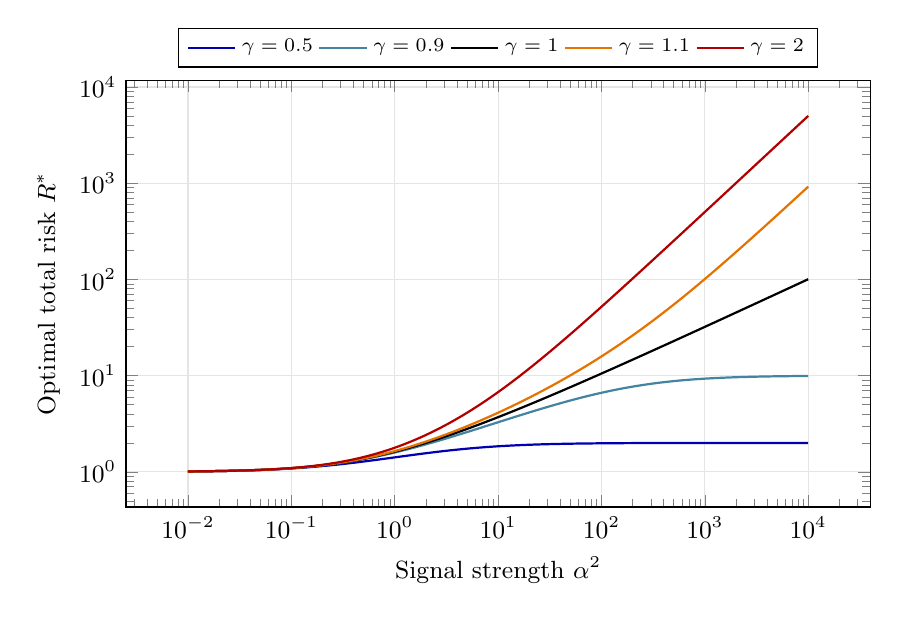
\begin{tikzpicture}
\begin{axis}[width=.91\linewidth,height=7cm,xmode=log,ymode=log,
xlabel={Signal strength $\alpha^2$},ylabel={Optimal total risk $R^*$},
grid=major,grid style={gray!20},
legend style={font=\scriptsize,at={(.5,1.03)},anchor=south,legend columns=5},
tick label style={font=\small},label style={font=\small}]
\addplot[thick,blue!70!black] coordinates {(0.01,1.0098058) (0.011911031,1.011637) (0.014187267,1.013801) (0.016898498,1.0163547) (0.020127854,1.0193632) (0.02397435,1.0229009) (0.028555923,1.0270516) (0.034013049,1.0319095) (0.04051305,1.0375785) (0.04825522,1.0441725) (0.057476944,1.0518141) (0.068460968,1.0606335) (0.081544074,1.0707658) (0.097127402,1.082348) (0.11568875,1.0955155) (0.13779724,1.1103972) (0.16413072,1.1271108) (0.19549661,1.1457567) (0.23285663,1.166413) (0.27735626,1.1891298) (0.33035991,1.2139243) (0.39349273,1.240776) (0.46869042,1.2696236) (0.55825863,1.3003618) (0.6649436,1.3328406) (0.79201641,1.3668644) (0.94337322,1.4021941) (1.1236548,1.43855) (1.3383888,1.4756169) (1.594159,1.5130515) (1.8988078,1.550491) (2.2616759,1.5875643) (2.6938893,1.6239042) (3.2087,1.6591603) (3.8218926,1.6930116) (4.5522683,1.7251783) (5.422221,1.755431) (6.4584244,1.7835971) (7.6926496,1.809564) (9.162739,1.833278) (10.913767,1.854741) (12.999422,1.8740033) (15.483653,1.8911553) (18.442627,1.9063186) (21.967071,1.9196358) (26.165047,1.9312628) (31.165269,1.9413604) (37.12105,1.9500888) (44.214999,1.9576025) (52.664624,1.9640473) (62.728999,1.9695579) (74.716707,1.974257) (88.995304,1.9782546) (106.00258,1.9816487) (126.26001,1.9845255) (150.38869,1.9869601) (179.12845,1.9890181) (213.36045,1.9907558) (254.1343,1.9922217) (302.70017,1.9934575) (360.54712,1.9944986) (429.4488,1.9953751) (511.51781,1.9961128) (609.27047,1.9967335) (725.70396,1.9972554) (864.38826,1.9976942) (1029.5756,1.9980631) (1226.3307,1.9983731) (1460.6863,1.9986336) (1739.8281,1.9988524) (2072.3146,1.9990363) (2468.3405,1.9991907) (2940.0481,1.9993204) (3501.9005,1.9994294) (4171.1246,1.9995209) (4968.2396,1.9995977) (5917.6857,1.9996622) (7048.574,1.9997164) (8395.5786,1.9997619) (10000,1.9998001)};
\addlegendentry{$\gamma=0.5$}
\addplot[thick,cyan!60!black] coordinates {(0.01,1.0098912) (0.011911031,1.0117572) (0.014187267,1.0139701) (0.016898498,1.016592) (0.020127854,1.0196959) (0.02397435,1.0233661) (0.028555923,1.0277007) (0.034013049,1.0328124) (0.04051305,1.0388305) (0.04825522,1.0459021) (0.057476944,1.0541939) (0.068460968,1.0638927) (0.081544074,1.0752066) (0.097127402,1.0883653) (0.11568875,1.1036197) (0.13779724,1.1212414) (0.16413072,1.1415215) (0.19549661,1.1647688) (0.23285663,1.1913081) (0.27735626,1.2214783) (0.33035991,1.2556299) (0.39349273,1.2941242) (0.46869042,1.3373311) (0.55825863,1.3856289) (0.6649436,1.4394037) (0.79201641,1.4990491) (0.94337322,1.5649666) (1.1236548,1.6375651) (1.3383888,1.7172612) (1.594159,1.804478) (1.8988078,1.8996436) (2.2616759,2.003189) (2.6938893,2.1155443) (3.2087,2.2371339) (3.8218926,2.3683703) (4.5522683,2.5096462) (5.422221,2.6613247) (6.4584244,2.8237281) (7.6926496,2.9971243) (9.162739,3.1817117) (10.913767,3.3776015) (12.999422,3.5847996) (15.483653,3.8031857) (18.442627,4.0324923) (21.967071,4.272284) (26.165047,4.5219368) (31.165269,4.7806201) (37.12105,5.0472831) (44.214999,5.3206459) (52.664624,5.5991994) (62.728999,5.8812149) (74.716707,6.1647654) (88.995304,6.4477602) (106.00258,6.7279936) (126.26001,7.0032062) (150.38869,7.2711571) (179.12845,7.5297028) (213.36045,7.7768772) (254.1343,8.0109667) (302.70017,8.230573) (360.54712,8.4346587) (429.4488,8.6225706) (511.51781,8.7940402) (609.27047,8.9491614) (725.70396,9.0883502) (864.38826,9.2122913) (1029.5756,9.3218764) (1226.3307,9.4181427) (1460.6863,9.5022143) (1739.8281,9.5752503) (2072.3146,9.6384026) (2468.3405,9.6927833) (2940.0481,9.7394412) (3501.9005,9.7793465) (4171.1246,9.8133832) (4968.2396,9.8423456) (5917.6857,9.8669402) (7048.574,9.8877893) (8395.5786,9.9054371) (10000,9.9203562)};
\addlegendentry{$\gamma=0.9$}
\addplot[thick,black] coordinates {(0.01,1.009902) (0.011911031,1.0117724) (0.014187267,1.0139915) (0.016898498,1.0166222) (0.020127854,1.0197383) (0.02397435,1.0234256) (0.028555923,1.027784) (0.034013049,1.0329287) (0.04051305,1.0389926) (0.04825522,1.0461275) (0.057476944,1.054506) (0.068460968,1.0643235) (0.081544074,1.0757986) (0.097127402,1.0891752) (0.11568875,1.104722) (0.13779724,1.1227337) (0.16413072,1.1435299) (0.19549661,1.1674553) (0.23285663,1.1948789) (0.27735626,1.226193) (0.33035991,1.2618136) (0.39349273,1.30218) (0.46869042,1.3477561) (0.55825863,1.399032) (0.6649436,1.4565268) (0.79201641,1.520792) (0.94337322,1.5924162) (1.1236548,1.6720302) (1.3383888,1.760313) (1.594159,1.8579982) (1.8988078,1.9658812) (2.2616759,2.0848268) (2.6938893,2.2157766) (3.2087,2.359758) (3.8218926,2.5178931) (4.5522683,2.6914078) (5.422221,2.8816425) (6.4584244,3.0900626) (7.6926496,3.3182707) (9.162739,3.5680187) (10.913767,3.8412224) (12.999422,4.1399756) (15.483653,4.4665668) (18.442627,4.8234971) (21.967071,5.2134988) (26.165047,5.6395571) (31.165269,6.1049326) (37.12105,6.6131866) (44.214999,7.1682081) (52.664624,7.7742439) (62.728999,8.4359309) (74.716707,9.1583316) (88.995304,9.9469732) (106.00258,10.807889) (126.26001,11.747667) (150.38869,12.773496) (179.12845,13.893224) (213.36045,15.115418) (254.1343,16.44943) (302.70017,17.905464) (360.54712,19.49466) (429.4488,21.229177) (511.51781,23.122286) (609.27047,25.188468) (725.70396,27.443533) (864.38826,29.904732) (1029.5756,32.590895) (1226.3307,35.522574) (1460.6863,38.722197) (1739.8281,42.214243) (2072.3146,46.025429) (2468.3405,50.184912) (2940.0481,54.724515) (3501.9005,59.67897) (4171.1246,65.08618) (4968.2396,70.987514) (5917.6857,77.428121) (7048.574,84.457275) (8395.5786,92.128754) (10000,100.50125)};
\addlegendentry{$\gamma=1$}
\addplot[thick,orange!90!black] coordinates {(0.01,1.0099108) (0.011911031,1.0117849) (0.014187267,1.0140091) (0.016898498,1.016647) (0.020127854,1.0197731) (0.02397435,1.0234745) (0.028555923,1.0278525) (0.034013049,1.0330245) (0.04051305,1.0391263) (0.04825522,1.0463135) (0.057476944,1.054764) (0.068460968,1.06468) (0.081544074,1.0762895) (0.097127402,1.0898481) (0.11568875,1.10564) (0.13779724,1.1239794) (0.16413072,1.1452111) (0.19549661,1.169711) (0.23285663,1.1978866) (0.27735626,1.2301781) (0.33035991,1.2670596) (0.39349273,1.3090413) (0.46869042,1.3566724) (0.55825863,1.4105461) (0.6649436,1.4713052) (0.79201641,1.5396499) (0.94337322,1.6163476) (1.1236548,1.7022434) (1.3383888,1.7982743) (1.594159,1.9054839) (1.8988078,2.0250407) (2.2616759,2.1582587) (2.6938893,2.306621) (3.2087,2.4718079) (3.8218926,2.6557289) (4.5522683,2.8605609) (5.422221,3.0887928) (6.4584244,3.3432784) (7.6926496,3.6272998) (9.162739,3.9446416) (10.913767,4.2996818) (12.999422,4.6974992) (15.483653,5.1440039) (18.442627,5.6460936) (21.967071,6.2118435) (26.165047,6.8507358) (31.165269,7.5739374) (37.12105,8.3946371) (44.214999,9.3284538) (52.664624,10.393932) (62.728999,11.61314) (74.716707,13.012395) (88.995304,14.62314) (106.00258,16.482989) (126.26001,18.636998) (150.38869,21.139171) (179.12845,24.054265) (213.36045,27.459934) (254.1343,31.449272) (302.70017,36.133829) (360.54712,41.647175) (429.4488,48.149111) (511.51781,55.830665) (609.27047,64.919991) (725.70396,75.689381) (864.38826,88.463587) (1029.5756,103.62972) (1226.3307,121.64905) (1460.6863,143.07104) (1739.8281,168.55011) (2072.3146,198.86559) (2468.3405,234.94551) (2940.0481,277.89501) (3501.9005,329.03013) (4171.1246,389.91809) (4968.2396,462.4253) (5917.6857,548.77457) (7048.574,651.6132) (8395.5786,774.09413) (10000,919.97263)};
\addlegendentry{$\gamma=1.1$}
\addplot[thick,red!70!black] coordinates {(0.01,1.0099507) (0.011911031,1.0118413) (0.014187267,1.0140887) (0.016898498,1.0167592) (0.020127854,1.0199312) (0.02397435,1.0236969) (0.028555923,1.0281648) (0.034013049,1.0334624) (0.04051305,1.0397388) (0.04825522,1.0471684) (0.057476944,1.0559541) (0.068460968,1.0663316) (0.081544074,1.0785738) (0.097127402,1.0929955) (0.11568875,1.1099584) (0.13779724,1.1298775) (0.16413072,1.1532269) (0.19549661,1.1805474) (0.23285663,1.2124552) (0.27735626,1.2496516) (0.33035991,1.2929357) (0.39349273,1.34322) (0.46869042,1.4015496) (0.55825863,1.4691261) (0.6649436,1.5473387) (0.79201641,1.6378008) (0.94337322,1.7423978) (1.1236548,1.8633432) (1.3383888,2.0032489) (1.594159,2.1652099) (1.8988078,2.3529065) (2.2616759,2.5707281) (2.6938893,2.8239213) (3.2087,3.1187679) (3.8218926,3.4627968) (4.5522683,3.8650376) (5.422221,4.3363204) (6.4584244,4.8896325) (7.6926496,5.5405396) (9.162739,6.307685) (10.913767,7.2133784) (12.999422,8.2842935) (15.483653,9.552294) (18.442627,11.055413) (21.967071,12.839017) (26.165047,14.957188) (31.165269,17.474377) (37.12105,20.46736) (44.214999,24.027588) (52.664624,28.263969) (62.728999,33.306201) (74.716707,39.308736) (88.995304,46.455507) (106.00258,54.965556) (126.26001,65.099748) (150.38869,77.168762) (179.12845,91.542611) (213.36045,108.66199) (254.1343,129.05177) (302.70017,153.33712) (360.54712,182.26264) (429.4488,216.71521) (511.51781,257.75118) (609.27047,306.62873) (725.70396,364.84651) (864.38826,434.18954) (1029.5756,516.78392) (1226.3307,615.1621) (1460.6863,732.34043) (1739.8281,871.91174) (2072.3146,1038.1554) (2468.3405,1236.1686) (2940.0481,1472.0227) (3501.9005,1752.9491) (4171.1246,2087.5613) (4968.2396,2486.119) (5917.6857,2960.8422) (7048.574,3526.2865) (8395.5786,4199.7888) (10000,5001.9996)};
\addlegendentry{$\gamma=2$}
\end{axis}\end{tikzpicture}
\caption{单位协方差下的强信号学习区间：每个点均使用 $\lambda^*=\gamma/\alpha^2$。本图选择 $\gamma\in\{0.5,0.9,1,1.1,2\}$，展示原论文图 3 的理论现象，并非其全部参数设置的逐点重绘。}
\label{fig:strongsignal}\end{figure}
\subsection{有限样本核验与讨论}
在 $\gamma=1$、$\lambda=1/\alpha^2$ 处，取 $n=p\in\{120,300,600\}$ 并独立重复抽取训练特征。表~\ref{tab:convergence}~显示各样本量下的条件风险均值均接近理论极限；这里考察的是渐近近似，随机误差不要求逐次单调下降。
\begin{table}[htbp]\centering\small
\caption{不同样本规模下的条件风险与高维极限。}\label{tab:convergence}
\begin{tabular}{cccc}\toprule
$n=p$ & 理论风险 & 条件风险均值 & 绝对差 \\ \midrule
$120$ & $1.618034$ & $1.618721$ & $0.000687$ \\
$300$ & $1.618034$ & $1.618327$ & $0.000293$ \\
$600$ & $1.618034$ & $1.618113$ & $0.000079$ \\
\bottomrule\end{tabular}\end{table}
直接线性方程求解与谱方法的最大系数差为 $1.25\times10^{-14}$，谱风险与迹风险的最大差为 $1.31\times10^{-13}$。固定训练特征后进行了 $4000$ 次系数与训练噪声重复，平均模型总体风险与精确条件风险的最大标准化偏差为 $1.50$，通过程序核验。
边界核验还包括无正则极限、零预测器风险、有限样本最优参数及过参数区的零特征值贡献。上述基础实验考察单位协方差，原文两种协方差模型的复现见下文。
复现代码为 \filename{A1_ridge_reproduction.py}，参数、原始数值和运行说明保存在同目录，四张图的坐标嵌入本文源文件。
% END A1 GENERATED RESULTS

% BEGIN A1 COVARIANCE RESULTS
\subsection{原文协方差模型的实验复现}\label{sec:covariance_experiments}
原文图 2 使用 BinaryTree 与 Exponential 两种总体协方差模型\cite{dw,authorcode}。本文按作者公开代码构造其特征值，采用谱等价表示 $\Sigma=\operatorname{diag}(t_1,\ldots,t_p)$ 和 $X=Z\Sigma^{1/2}$。由于高斯系数分布及岭惩罚具有旋转不变性，该表示保留预测风险的分布；两种模型的训练和测试特征均为高斯变量，模型名称描述的是协方差谱。
BinaryTree 取深度 $d=4$，因此 $p=2^d-1=15$，按 $n=\lfloor p/\gamma_0\rfloor$ 选择样本量；Exponential 固定 $n=20$，按 $p=\lfloor n\gamma_0\rfloor$ 选择维数，指数率为 $1$。$\gamma_0$ 是目标比值，所有理论和最优参数计算均使用实际 $\gamma=p/n$。
两模型的正则扫描取 $\gamma_0\in\{0.5,1,2\}$，信号强度 $\alpha^2=1$、噪声方差 $1$，每组独立重复 $500$ 次，每次测试集大小为 $100$；随机种子为 20261004。BinaryTree 的 $\sqrt{\lambda}$ 网格为 $[0.1,\sqrt{10}]$，Exponential 为 $[0.1,2.5]$，各取 $50$ 点并加入实际最优点。
理论曲线以有限总体谱 $H_p=p^{-1}\sum_i\delta_{t_i}$ 代入式~\eqref{eq:generalrisk}，采用式~\eqref{eq:companion_solver}~的正根计算，是确定性等价近似；精确条件风险另由式~\eqref{eq:weightedrisk}~计算。维数扫描保持同一协方差构造规则，取 $\gamma_0\in[0.25,2.5]$、固定 $\lambda\in\{0.1,1,4\}$，用于补充原文固定比值的正则扫描。
与原文的对应关系需要说明：论文图注写 BinaryTree 的 $p=2^4$，公开代码采用 $p=2^d-1$；本文遵循代码并报告实际比值。公开模拟函数采用 $500$ 次训练重复、每次 $100$ 个测试点，正文与图注的配置记载并不完全一致。本文共享同次重复内不同正则参数的训练和测试数据，边际实验设定一致，随机波动及网格与原图不要求逐点相同。
图~\ref{fig:covlambda}~直接对应原文的六个正则路径面板；图~\ref{fig:covgamma}~考察固定正则下的维数变化。两图统一比较总预测风险，其噪声底座为 $1$。
\begin{figure}[p]\centering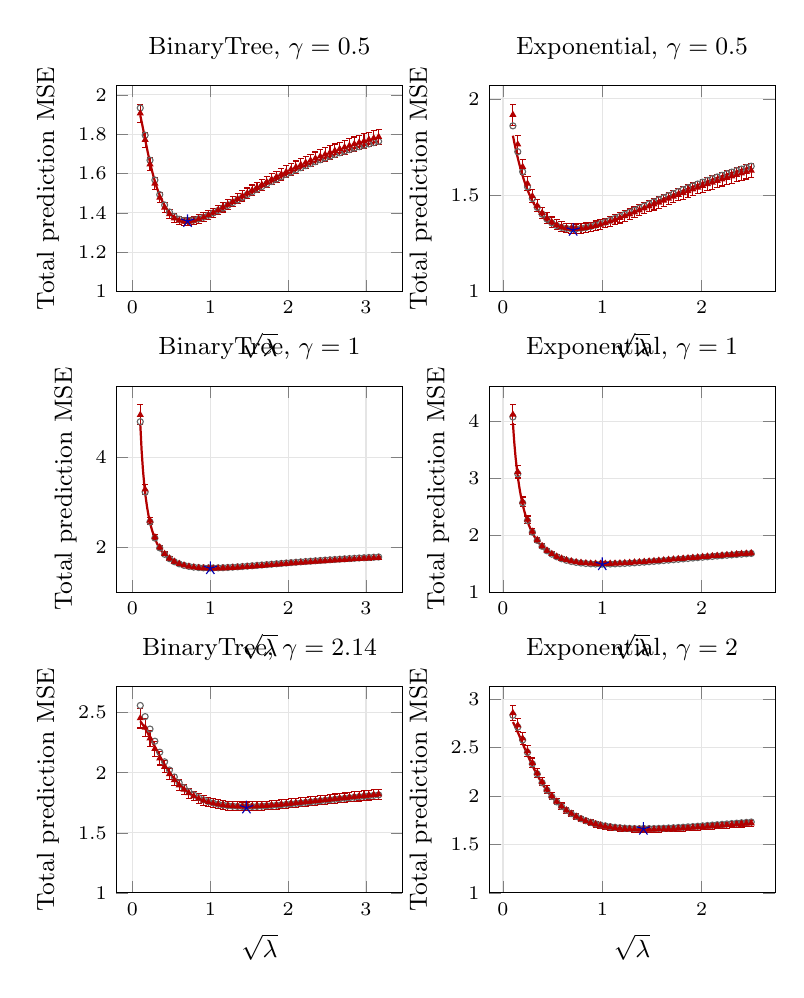
\begin{tikzpicture}
\begin{groupplot}[group style={group size=2 by 3,horizontal sep=1.1cm,vertical sep=1.2cm},
width=.43\linewidth,height=4.2cm,grid=major,grid style={gray!20},
xlabel={$\sqrt{\lambda}$},ylabel={Total prediction MSE},ymin=1,
tick label style={font=\scriptsize},label style={font=\small},
title style={font=\small}]
\nextgroupplot[title={BinaryTree, $\gamma=0.5$}]
\addplot[thick,red!70!black] coordinates {(0.1,1.8953359) (0.1171077,1.8632455) (0.13421539,1.8296722) (0.15132309,1.7954936) (0.16843079,1.761439) (0.18553848,1.7280856) (0.20264618,1.6958681) (0.21975387,1.6650958) (0.23686157,1.6359736) (0.25396927,1.6086221) (0.27107696,1.5830961) (0.28818466,1.5594015) (0.30529236,1.537508) (0.32240005,1.5173603) (0.33950775,1.4988861) (0.35661545,1.4820028) (0.37372314,1.4666222) (0.39083084,1.4526538) (0.40793854,1.4400075) (0.42504623,1.4285953) (0.44215393,1.4183324) (0.45926162,1.4091379) (0.47636932,1.4009354) (0.49347702,1.393653) (0.51058471,1.3872234) (0.52769241,1.381584) (0.54480011,1.3766762) (0.5619078,1.3724459) (0.5790155,1.368843) (0.5961232,1.3658208) (0.61323089,1.3633364) (0.63033859,1.3613499) (0.64744629,1.3598245) (0.66455398,1.3587261) (0.68166168,1.3580233) (0.69876937,1.3576869) (0.71587707,1.35769) (0.73298477,1.3580076) (0.75009246,1.3586166) (0.76720016,1.3594956) (0.78430786,1.3606247) (0.80141555,1.3619855) (0.81852325,1.3635609) (0.83563095,1.365335) (0.85273864,1.3672931) (0.86984634,1.3694214) (0.88695404,1.3717072) (0.90406173,1.3741386) (0.92116943,1.3767046) (0.93827712,1.3793947) (0.95538482,1.3821994) (0.97249252,1.3851098) (0.98960021,1.3881173) (1.0067079,1.3912142) (1.0238156,1.3943932) (1.0409233,1.3976474) (1.058031,1.4009704) (1.0751387,1.4043562) (1.0922464,1.4077992) (1.1093541,1.4112941) (1.1264618,1.4148361) (1.1435695,1.4184204) (1.1606772,1.4220428) (1.1777849,1.4256991) (1.1948926,1.4293856) (1.2120003,1.4330987) (1.229108,1.436835) (1.2462157,1.4405914) (1.2633234,1.4443649) (1.2804311,1.4481526) (1.2975387,1.4519521) (1.3146464,1.4557608) (1.3317541,1.4595763) (1.3488618,1.4633967) (1.3659695,1.4672197) (1.3830772,1.4710434) (1.4001849,1.4748662) (1.4172926,1.4786862) (1.4344003,1.4825018) (1.451508,1.4863117) (1.4686157,1.4901143) (1.4857234,1.4939084) (1.5028311,1.4976927) (1.5199388,1.501466) (1.5370465,1.5052273) (1.5541542,1.5089755) (1.5712619,1.5127098) (1.5883696,1.5164291) (1.6054773,1.5201326) (1.622585,1.5238196) (1.6396927,1.5274894) (1.6568004,1.5311411) (1.6739081,1.5347743) (1.6910158,1.5383883) (1.7081235,1.5419826) (1.7252312,1.5455566) (1.7423389,1.5491099) (1.7594466,1.5526421) (1.7765542,1.5561527) (1.7936619,1.5596413) (1.8107696,1.5631076) (1.8278773,1.5665514) (1.844985,1.5699722) (1.8620927,1.5733699) (1.8792004,1.5767442) (1.8963081,1.5800949) (1.9134158,1.5834218) (1.9305235,1.5867247) (1.9476312,1.5900035) (1.9647389,1.5932581) (1.9818466,1.5964882) (1.9989543,1.5996939) (2.016062,1.6028751) (2.0331697,1.6060316) (2.0502774,1.6091635) (2.0673851,1.6122707) (2.0844928,1.6153531) (2.1016005,1.6184108) (2.1187082,1.6214437) (2.1358159,1.6244519) (2.1529236,1.6274354) (2.1700313,1.6303942) (2.187139,1.6333283) (2.2042467,1.6362379) (2.2213544,1.6391229) (2.2384621,1.6419834) (2.2555697,1.6448195) (2.2726774,1.6476313) (2.2897851,1.6504188) (2.3068928,1.6531823) (2.3240005,1.6559216) (2.3411082,1.658637) (2.3582159,1.6613286) (2.3753236,1.6639965) (2.3924313,1.6666408) (2.409539,1.6692616) (2.4266467,1.671859) (2.4437544,1.6744332) (2.4608621,1.6769844) (2.4779698,1.6795126) (2.4950775,1.682018) (2.5121852,1.6845008) (2.5292929,1.686961) (2.5464006,1.6893989) (2.5635083,1.6918146) (2.580616,1.6942082) (2.5977237,1.6965799) (2.6148314,1.6989299) (2.6319391,1.7012583) (2.6490468,1.7035653) (2.6661545,1.7058511) (2.6832622,1.7081157) (2.7003699,1.7103594) (2.7174776,1.7125824) (2.7345852,1.7147847) (2.7516929,1.7169666) (2.7688006,1.7191283) (2.7859083,1.7212699) (2.803016,1.7233915) (2.8201237,1.7254934) (2.8372314,1.7275757) (2.8543391,1.7296385) (2.8714468,1.7316822) (2.8885545,1.7337067) (2.9056622,1.7357123) (2.9227699,1.7376992) (2.9398776,1.7396675) (2.9569853,1.7416174) (2.974093,1.743549) (2.9912007,1.7454625) (3.0083084,1.7473582) (3.0254161,1.7492361) (3.0425238,1.7510964) (3.0596315,1.7529393) (3.0767392,1.754765) (3.0938469,1.7565736) (3.1109546,1.7583652) (3.1280623,1.7601401) (3.14517,1.7618984) (3.1622777,1.7636402)};
\addplot[only marks,mark=o,mark size=1.1pt,black!60] coordinates {(0.1,1.9331474) (0.16249546,1.7946621) (0.22499092,1.6676402) (0.28748639,1.5670008) (0.34998185,1.492694) (0.41247731,1.4401457) (0.47497277,1.4044178) (0.53746824,1.3813846) (0.5999637,1.3678681) (0.66245916,1.3614874) (0.70710678,1.3602981) (0.72495462,1.3604709) (0.78745009,1.3634965) (0.84994555,1.3695703) (0.91244101,1.3779394) (0.97493647,1.3880274) (1.0374319,1.39939) (1.0999274,1.4116813) (1.1624229,1.4246305) (1.2249183,1.4380243) (1.2874138,1.4516936) (1.3499092,1.4655043) (1.4124047,1.4793495) (1.4749002,1.4931442) (1.5373956,1.5068206) (1.5998911,1.5203251) (1.6623866,1.5336155) (1.724882,1.5466589) (1.7873775,1.5594297) (1.8498729,1.571909) (1.9123684,1.5840828) (1.9748639,1.5959412) (2.0373593,1.6074782) (2.0998548,1.6186903) (2.1623503,1.6295766) (2.2248457,1.6401381) (2.2873412,1.6503776) (2.3498366,1.6602988) (2.4123321,1.6699069) (2.4748276,1.6792076) (2.537323,1.6882076) (2.5998185,1.6969138) (2.662314,1.7053337) (2.7248094,1.713475) (2.7873049,1.7213456) (2.8498003,1.7289535) (2.9122958,1.7363068) (2.9747913,1.7434136) (3.0372867,1.7502819) (3.0997822,1.7569196) (3.1622777,1.7633346)};
\addplot[only marks,mark=triangle*,mark size=1.1pt,red!70!black,error bars/.cd,y dir=both,y explicit] coordinates {(0.1,1.9059852) +- (0,0.046345677) (0.16249546,1.7712433) +- (0,0.038706437) (0.22499092,1.6472898) +- (0,0.032821401) (0.28748639,1.5493571) +- (0,0.028787075) (0.34998185,1.4775617) +- (0,0.026093152) (0.41247731,1.4273499) +- (0,0.02430785) (0.47497277,1.3937684) +- (0,0.023144767) (0.53746824,1.3726845) +- (0,0.022416347) (0.5999637,1.3609272) +- (0,0.021996417) (0.66245916,1.3561326) +- (0,0.021798519) (0.70710678,1.355982) +- (0,0.021759205) (0.72495462,1.35655) +- (0,0.021762882) (0.78745009,1.3608789) +- (0,0.021847894) (0.84994555,1.3681461) +- (0,0.022024264) (0.91244101,1.3776166) +- (0,0.022271029) (0.97493647,1.38873) +- (0,0.022572835) (1.0374319,1.4010553) +- (0,0.022918131) (1.0999274,1.4142578) +- (0,0.02329798) (1.1624229,1.4280759) +- (0,0.023705282) (1.2249183,1.4423038) +- (0,0.024134267) (1.2874138,1.4567785) +- (0,0.024580162) (1.3499092,1.4713706) +- (0,0.025038975) (1.4124047,1.485977) +- (0,0.025507333) (1.4749002,1.5005156) +- (0,0.025982378) (1.5373956,1.5149209) +- (0,0.026461682) (1.5998911,1.5291409) +- (0,0.026943179) (1.6623866,1.5431345) +- (0,0.027425112) (1.724882,1.5568696) +- (0,0.027905988) (1.7873775,1.5703212) +- (0,0.02838454) (1.8498729,1.5834707) +- (0,0.028859694) (1.9123684,1.596304) +- (0,0.02933054) (1.9748639,1.6088116) +- (0,0.02979631) (2.0373593,1.620987) +- (0,0.030256356) (2.0998548,1.6328269) +- (0,0.030710134) (2.1623503,1.6443301) +- (0,0.031157188) (2.2248457,1.6554976) +- (0,0.031597142) (2.2873412,1.6663316) +- (0,0.032029684) (2.3498366,1.6768361) +- (0,0.032454562) (2.4123321,1.6870159) +- (0,0.032871573) (2.4748276,1.6968768) +- (0,0.033280561) (2.537323,1.706425) +- (0,0.033681409) (2.5998185,1.7156678) +- (0,0.034074033) (2.662314,1.7246123) +- (0,0.034458384) (2.7248094,1.7332664) +- (0,0.034834436) (2.7873049,1.7416379) +- (0,0.035202191) (2.8498003,1.749735) +- (0,0.035561672) (2.9122958,1.7575658) +- (0,0.035912919) (2.9747913,1.7651384) +- (0,0.036255993) (3.0372867,1.7724609) +- (0,0.036590968) (3.0997822,1.7795415) +- (0,0.036917932) (3.1622777,1.7863881) +- (0,0.037236984)};
\addplot[only marks,mark=star,mark size=2.5pt,blue!70!black] coordinates {(0.70710678,1.3576476)};
\nextgroupplot[title={Exponential, $\gamma=0.5$}]
\addplot[thick,red!70!black] coordinates {(0.1,1.8090741) (0.11340782,1.7754289) (0.12681564,1.7432232) (0.14022346,1.7126828) (0.15363128,1.683891) (0.16703911,1.656846) (0.18044693,1.6314983) (0.19385475,1.6077736) (0.20726257,1.5855868) (0.22067039,1.56485) (0.23407821,1.5454762) (0.24748603,1.5273817) (0.26089385,1.5104876) (0.27430168,1.4947193) (0.2877095,1.4800073) (0.30111732,1.4662866) (0.31452514,1.4534967) (0.32793296,1.4415811) (0.34134078,1.4304874) (0.3547486,1.4201665) (0.36815642,1.4105729) (0.38156425,1.4016641) (0.39497207,1.3934004) (0.40837989,1.3857448) (0.42178771,1.3786627) (0.43519553,1.3721219) (0.44860335,1.3660923) (0.46201117,1.3605454) (0.47541899,1.3554551) (0.48882682,1.3507964) (0.50223464,1.3465461) (0.51564246,1.3426825) (0.52905028,1.3391852) (0.5424581,1.3360348) (0.55586592,1.3332133) (0.56927374,1.3307037) (0.58268156,1.3284899) (0.59608939,1.326557) (0.60949721,1.3248905) (0.62290503,1.323477) (0.63631285,1.3223039) (0.64972067,1.3213591) (0.66312849,1.3206313) (0.67653631,1.3201096) (0.68994413,1.3197839) (0.70335196,1.3196446) (0.71675978,1.3196825) (0.7301676,1.3198888) (0.74357542,1.3202553) (0.75698324,1.3207742) (0.77039106,1.3214379) (0.78379888,1.3222395) (0.7972067,1.3231721) (0.81061453,1.3242293) (0.82402235,1.325405) (0.83743017,1.3266933) (0.85083799,1.3280887) (0.86424581,1.3295858) (0.87765363,1.3311796) (0.89106145,1.3328652) (0.90446927,1.334638) (0.91787709,1.3364935) (0.93128492,1.3384276) (0.94469274,1.3404362) (0.95810056,1.3425154) (0.97150838,1.3446615) (0.9849162,1.346871) (0.99832402,1.3491405) (1.0117318,1.3514667) (1.0251397,1.3538466) (1.0385475,1.356277) (1.0519553,1.3587553) (1.0653631,1.3612786) (1.0787709,1.3638444) (1.0921788,1.36645) (1.1055866,1.3690931) (1.1189944,1.3717713) (1.1324022,1.3744825) (1.1458101,1.3772245) (1.1592179,1.3799953) (1.1726257,1.3827928) (1.1860335,1.3856153) (1.1994413,1.3884608) (1.2128492,1.3913277) (1.226257,1.3942142) (1.2396648,1.3971189) (1.2530726,1.4000401) (1.2664804,1.4029763) (1.2798883,1.4059262) (1.2932961,1.4088884) (1.3067039,1.4118615) (1.3201117,1.4148443) (1.3335196,1.4178357) (1.3469274,1.4208344) (1.3603352,1.4238394) (1.373743,1.4268496) (1.3871508,1.4298639) (1.4005587,1.4328814) (1.4139665,1.4359011) (1.4273743,1.4389221) (1.4407821,1.4419436) (1.4541899,1.4449648) (1.4675978,1.4479848) (1.4810056,1.4510029) (1.4944134,1.4540183) (1.5078212,1.4570303) (1.5212291,1.4600383) (1.5346369,1.4630417) (1.5480447,1.4660398) (1.5614525,1.4690319) (1.5748603,1.4720177) (1.5882682,1.4749965) (1.601676,1.4779677) (1.6150838,1.480931) (1.6284916,1.4838859) (1.6418994,1.4868318) (1.6553073,1.4897684) (1.6687151,1.4926952) (1.6821229,1.495612) (1.6955307,1.4985182) (1.7089385,1.5014136) (1.7223464,1.5042978) (1.7357542,1.5071704) (1.749162,1.5100313) (1.7625698,1.5128801) (1.7759777,1.5157165) (1.7893855,1.5185402) (1.8027933,1.5213511) (1.8162011,1.5241489) (1.8296089,1.5269334) (1.8430168,1.5297044) (1.8564246,1.5324616) (1.8698324,1.5352049) (1.8832402,1.5379342) (1.896648,1.5406492) (1.9100559,1.5433498) (1.9234637,1.5460359) (1.9368715,1.5487074) (1.9502793,1.5513641) (1.9636872,1.5540059) (1.977095,1.5566327) (1.9905028,1.5592444) (2.0039106,1.561841) (2.0173184,1.5644223) (2.0307263,1.5669883) (2.0441341,1.569539) (2.0575419,1.5720742) (2.0709497,1.5745939) (2.0843575,1.577098) (2.0977654,1.5795866) (2.1111732,1.5820596) (2.124581,1.584517) (2.1379888,1.5869587) (2.1513966,1.5893847) (2.1648045,1.5917951) (2.1782123,1.5941898) (2.1916201,1.5965688) (2.2050279,1.5989322) (2.2184358,1.6012798) (2.2318436,1.6036118) (2.2452514,1.6059282) (2.2586592,1.608229) (2.272067,1.6105141) (2.2854749,1.6127837) (2.2988827,1.6150377) (2.3122905,1.6172763) (2.3256983,1.6194993) (2.3391061,1.621707) (2.352514,1.6238992) (2.3659218,1.6260761) (2.3793296,1.6282378) (2.3927374,1.6303841) (2.4061453,1.6325153) (2.4195531,1.6346314) (2.4329609,1.6367324) (2.4463687,1.6388183) (2.4597765,1.6408893) (2.4731844,1.6429455) (2.4865922,1.6449867) (2.5,1.6470133)};
\addplot[only marks,mark=o,mark size=1.1pt,black!60] coordinates {(0.1,1.8599914) (0.14897959,1.725734) (0.19795918,1.6222073) (0.24693878,1.5432743) (0.29591837,1.4829733) (0.34489796,1.4369116) (0.39387755,1.4019109) (0.44285714,1.3756304) (0.49183673,1.3563105) (0.54081633,1.3426046) (0.58979592,1.3334655) (0.63877551,1.3280668) (0.6877551,1.3257479) (0.70710678,1.3255594) (0.73673469,1.3259744) (0.78571429,1.3283096) (0.83469388,1.3323928) (0.88367347,1.3379242) (0.93265306,1.3446525) (0.98163265,1.3523656) (1.0306122,1.360884) (1.0795918,1.370055) (1.1285714,1.3797478) (1.177551,1.389851) (1.2265306,1.4002684) (1.2755102,1.410918) (1.3244898,1.4217287) (1.3734694,1.43264) (1.422449,1.4435995) (1.4714286,1.4545626) (1.5204082,1.4654909) (1.5693878,1.4763519) (1.6183673,1.4871176) (1.6673469,1.4977648) (1.7163265,1.5082737) (1.7653061,1.5186279) (1.8142857,1.5288139) (1.8632653,1.5388206) (1.9122449,1.5486392) (1.9612245,1.5582627) (2.0102041,1.567686) (2.0591837,1.5769053) (2.1081633,1.5859181) (2.1571429,1.5947229) (2.2061224,1.6033193) (2.255102,1.6117078) (2.3040816,1.6198893) (2.3530612,1.6278656) (2.4020408,1.6356389) (2.4510204,1.6432118) (2.5,1.6505873)};
\addplot[only marks,mark=triangle*,mark size=1.1pt,red!70!black,error bars/.cd,y dir=both,y explicit] coordinates {(0.1,1.917761) +- (0,0.05481786) (0.14897959,1.7638596) +- (0,0.045727247) (0.19795918,1.647497) +- (0,0.039838087) (0.24693878,1.5605191) +- (0,0.035781829) (0.29591837,1.4951747) +- (0,0.032838757) (0.34489796,1.445894) +- (0,0.030633885) (0.39387755,1.4087709) +- (0,0.028956499) (0.44285714,1.3810172) +- (0,0.027675966) (0.49183673,1.3605969) +- (0,0.026703897) (0.54081633,1.3459928) +- (0,0.025976564) (0.58979592,1.3360535) +- (0,0.025446139) (0.63877551,1.3298904) +- (0,0.02507587) (0.6877551,1.326808) +- (0,0.024837117) (0.70710678,1.3263137) +- (0,0.024773904) (0.73673469,1.3262538) +- (0,0.024707339) (0.78571429,1.3277837) +- (0,0.024668635) (0.83469388,1.3310364) +- (0,0.024706652) (0.88367347,1.3357149) +- (0,0.024809752) (0.93265306,1.3415728) +- (0,0.02496838) (0.98163265,1.3484042) +- (0,0.025174594) (1.0306122,1.3560354) +- (0,0.025421699) (1.0795918,1.3643195) +- (0,0.02570398) (1.1285714,1.3731313) +- (0,0.026016503) (1.177551,1.3823637) +- (0,0.026354961) (1.2265306,1.3919249) +- (0,0.026715566) (1.2755102,1.401736) +- (0,0.027094958) (1.3244898,1.4117289) +- (0,0.027490145) (1.3734694,1.4218452) +- (0,0.027898451) (1.422449,1.4320343) +- (0,0.028317477) (1.4714286,1.4422528) +- (0,0.028745068) (1.5204082,1.4524631) +- (0,0.02917929) (1.5693878,1.4626332) +- (0,0.029618404) (1.6183673,1.4727355) +- (0,0.030060851) (1.6673469,1.4827465) +- (0,0.030505234) (1.7163265,1.4926464) +- (0,0.030950304) (1.7653061,1.5024183) +- (0,0.031394947) (1.8142857,1.5120481) +- (0,0.031838172) (1.8632653,1.5215241) +- (0,0.0322791) (1.9122449,1.5308368) +- (0,0.032716955) (1.9612245,1.5399786) +- (0,0.033151056) (2.0102041,1.5489432) +- (0,0.033580805) (2.0591837,1.5577261) +- (0,0.034005682) (2.1081633,1.5663239) +- (0,0.034425238) (2.1571429,1.5747344) +- (0,0.034839089) (2.2061224,1.582956) +- (0,0.035246907) (2.255102,1.5909884) +- (0,0.035648417) (2.3040816,1.5988318) +- (0,0.036043392) (2.3530612,1.606487) +- (0,0.036431649) (2.4020408,1.6139555) +- (0,0.036813039) (2.4510204,1.6212389) +- (0,0.037187453) (2.5,1.6283396) +- (0,0.037554808)};
\addplot[only marks,mark=star,mark size=2.5pt,blue!70!black] coordinates {(0.70710678,1.3196377)};
\nextgroupplot[title={BinaryTree, $\gamma=1$}]
\addplot[thick,red!70!black] coordinates {(0.1,4.7368029) (0.1171077,4.1530184) (0.13421539,3.7206454) (0.15132309,3.3883077) (0.16843079,3.125502) (0.18553848,2.9129755) (0.20264618,2.7379762) (0.21975387,2.5917233) (0.23686157,2.4679726) (0.25396927,2.3621625) (0.27107696,2.2708827) (0.28818466,2.1915329) (0.30529236,2.1220956) (0.32240005,2.0609816) (0.33950775,2.0069219) (0.35661545,1.9588912) (0.37372314,1.916052) (0.39083084,1.8777134) (0.40793854,1.8433004) (0.42504623,1.8123308) (0.44215393,1.784397) (0.45926162,1.759152) (0.47636932,1.736299) (0.49347702,1.7155823) (0.51058471,1.6967803) (0.52769241,1.6797006) (0.54480011,1.6641746) (0.5619078,1.6500546) (0.5790155,1.6372102) (0.5961232,1.625526) (0.61323089,1.6148997) (0.63033859,1.60524) (0.64744629,1.5964654) (0.66455398,1.5885027) (0.68166168,1.5812861) (0.69876937,1.5747565) (0.71587707,1.5688601) (0.73298477,1.5635485) (0.75009246,1.5587776) (0.76720016,1.5545073) (0.78430786,1.550701) (0.80141555,1.5473252) (0.81852325,1.5443494) (0.83563095,1.5417456) (0.85273864,1.5394878) (0.86984634,1.5375525) (0.88695404,1.5359176) (0.90406173,1.5345631) (0.92116943,1.5334703) (0.93827712,1.5326219) (0.95538482,1.5320019) (0.97249252,1.5315953) (0.98960021,1.5313885) (1.0067079,1.5313686) (1.0238156,1.5315236) (1.0409233,1.5318423) (1.058031,1.5323144) (1.0751387,1.5329301) (1.0922464,1.5336803) (1.1093541,1.5345565) (1.1264618,1.5355507) (1.1435695,1.5366555) (1.1606772,1.5378638) (1.1777849,1.5391691) (1.1948926,1.5405651) (1.2120003,1.5420461) (1.229108,1.5436066) (1.2462157,1.5452413) (1.2633234,1.5469455) (1.2804311,1.5487146) (1.2975387,1.5505442) (1.3146464,1.5524303) (1.3317541,1.554369) (1.3488618,1.5563567) (1.3659695,1.55839) (1.3830772,1.5604655) (1.4001849,1.5625802) (1.4172926,1.5647313) (1.4344003,1.5669159) (1.451508,1.5691314) (1.4686157,1.5713755) (1.4857234,1.5736456) (1.5028311,1.5759397) (1.5199388,1.5782556) (1.5370465,1.5805913) (1.5541542,1.582945) (1.5712619,1.5853148) (1.5883696,1.587699) (1.6054773,1.5900961) (1.622585,1.5925044) (1.6396927,1.5949226) (1.6568004,1.5973493) (1.6739081,1.5997831) (1.6910158,1.6022228) (1.7081235,1.6046672) (1.7252312,1.6071152) (1.7423389,1.6095658) (1.7594466,1.6120179) (1.7765542,1.6144707) (1.7936619,1.616923) (1.8107696,1.6193742) (1.8278773,1.6218234) (1.844985,1.6242698) (1.8620927,1.6267127) (1.8792004,1.6291514) (1.8963081,1.6315852) (1.9134158,1.6340135) (1.9305235,1.6364358) (1.9476312,1.6388514) (1.9647389,1.6412598) (1.9818466,1.6436606) (1.9989543,1.6460532) (2.016062,1.6484372) (2.0331697,1.6508122) (2.0502774,1.6531778) (2.0673851,1.6555336) (2.0844928,1.6578792) (2.1016005,1.6602144) (2.1187082,1.6625388) (2.1358159,1.6648522) (2.1529236,1.6671541) (2.1700313,1.6694445) (2.187139,1.671723) (2.2042467,1.6739895) (2.2213544,1.6762436) (2.2384621,1.6784853) (2.2555697,1.6807143) (2.2726774,1.6829305) (2.2897851,1.6851337) (2.3068928,1.6873237) (2.3240005,1.6895005) (2.3411082,1.6916639) (2.3582159,1.6938138) (2.3753236,1.6959502) (2.3924313,1.6980728) (2.409539,1.7001817) (2.4266467,1.7022767) (2.4437544,1.7043578) (2.4608621,1.706425) (2.4779698,1.7084782) (2.4950775,1.7105173) (2.5121852,1.7125423) (2.5292929,1.7145532) (2.5464006,1.71655) (2.5635083,1.7185327) (2.580616,1.7205012) (2.5977237,1.7224555) (2.6148314,1.7243957) (2.6319391,1.7263218) (2.6490468,1.7282337) (2.6661545,1.7301315) (2.6832622,1.7320152) (2.7003699,1.7338848) (2.7174776,1.7357404) (2.7345852,1.737582) (2.7516929,1.7394096) (2.7688006,1.7412232) (2.7859083,1.743023) (2.803016,1.7448089) (2.8201237,1.746581) (2.8372314,1.7483394) (2.8543391,1.7500841) (2.8714468,1.7518152) (2.8885545,1.7535326) (2.9056622,1.7552366) (2.9227699,1.7569271) (2.9398776,1.7586042) (2.9569853,1.760268) (2.974093,1.7619186) (2.9912007,1.7635559) (3.0083084,1.7651802) (3.0254161,1.7667914) (3.0425238,1.7683897) (3.0596315,1.7699751) (3.0767392,1.7715476) (3.0938469,1.7731075) (3.1109546,1.7746547) (3.1280623,1.7761893) (3.14517,1.7777114) (3.1622777,1.7792211)};
\addplot[only marks,mark=o,mark size=1.1pt,black!60] coordinates {(0.1,4.7912966) (0.16249546,3.228607) (0.22499092,2.5643333) (0.28748639,2.205056) (0.34998185,1.9863007) (0.41247731,1.8436689) (0.47497277,1.7466994) (0.53746824,1.6791187) (0.5999637,1.6314495) (0.66245916,1.5978028) (0.72495462,1.5743296) (0.78745009,1.5584103) (0.84994555,1.5482019) (0.91244101,1.5423719) (0.97493647,1.5399339) (1,1.5397354) (1.0374319,1.5401439) (1.0999274,1.5424308) (1.1624229,1.5463501) (1.2249183,1.5515518) (1.2874138,1.5577571) (1.3499092,1.5647423) (1.4124047,1.5723261) (1.4749002,1.5803614) (1.5373956,1.5887276) (1.5998911,1.5973259) (1.6623866,1.6060748) (1.724882,1.6149074) (1.7873775,1.6237685) (1.8498729,1.6326125) (1.9123684,1.6414021) (1.9748639,1.6501066) (2.0373593,1.6587012) (2.0998548,1.6671658) (2.1623503,1.6754841) (2.2248457,1.6836435) (2.2873412,1.6916342) (2.3498366,1.6994487) (2.4123321,1.7070816) (2.4748276,1.7145293) (2.537323,1.7217896) (2.5998185,1.7288616) (2.662314,1.7357454) (2.7248094,1.7424418) (2.7873049,1.7489527) (2.8498003,1.7552802) (2.9122958,1.7614272) (2.9747913,1.7673966) (3.0372867,1.7731921) (3.0997822,1.7788174) (3.1622777,1.7842762)};
\addplot[only marks,mark=triangle*,mark size=1.1pt,red!70!black,error bars/.cd,y dir=both,y explicit] coordinates {(0.1,4.9426419) +- (0,0.2234345) (0.16249546,3.2859871) +- (0,0.11501647) (0.22499092,2.5943244) +- (0,0.075989862) (0.28748639,2.2245657) +- (0,0.057284459) (0.34998185,2.0003215) +- (0,0.047019277) (0.41247731,1.8537852) +- (0,0.040826467) (0.47497277,1.7535087) +- (0,0.036805843) (0.53746824,1.6829585) +- (0,0.034047975) (0.5999637,1.6326075) +- (0,0.032083617) (0.66245916,1.5965646) +- (0,0.030653343) (0.72495462,1.5709788) +- (0,0.029603986) (0.78745009,1.5532184) +- (0,0.028839247) (0.84994555,1.5414192) +- (0,0.028294845) (0.91244101,1.5342224) +- (0,0.02792542) (0.97493647,1.5306135) +- (0,0.027697341) (1,1.5299941) +- (0,0.027639543) (1.0374319,1.5298206) +- (0,0.027584626) (1.0999274,1.5312472) +- (0,0.027566561) (1.1624229,1.5344257) +- (0,0.02762625) (1.2249183,1.538986) +- (0,0.02774971) (1.2874138,1.5446321) +- (0,0.027925262) (1.3499092,1.5511259) +- (0,0.028143111) (1.4124047,1.558274) +- (0,0.028395021) (1.4749002,1.5659193) +- (0,0.028674071) (1.5373956,1.5739329) +- (0,0.028974446) (1.5998911,1.5822093) +- (0,0.029291266) (1.6623866,1.5906616) +- (0,0.029620447) (1.724882,1.5992185) +- (0,0.029958569) (1.7873775,1.6078211) +- (0,0.03030278) (1.8498729,1.6164211) +- (0,0.030650702) (1.9123684,1.6249787) +- (0,0.031000357) (1.9748639,1.6334617) +- (0,0.031350102) (2.0373593,1.6418435) +- (0,0.031698578) (2.0998548,1.650103) +- (0,0.032044665) (2.1623503,1.6582229) +- (0,0.032387441) (2.2248457,1.6661901) +- (0,0.032726152) (2.2873412,1.6739938) +- (0,0.033060188) (2.3498366,1.6816265) +- (0,0.033389054) (2.4123321,1.6890822) +- (0,0.033712361) (2.4748276,1.696357) +- (0,0.034029801) (2.537323,1.7034486) +- (0,0.034341139) (2.5998185,1.7103559) +- (0,0.034646201) (2.662314,1.7170787) +- (0,0.034944865) (2.7248094,1.723618) +- (0,0.035237049) (2.7873049,1.7299753) +- (0,0.035522713) (2.8498003,1.7361527) +- (0,0.035801843) (2.9122958,1.742153) +- (0,0.036074455) (2.9747913,1.7479793) +- (0,0.036340583) (3.0372867,1.7536349) +- (0,0.036600284) (3.0997822,1.7591235) +- (0,0.036853627) (3.1622777,1.7644489) +- (0,0.037100694)};
\addplot[only marks,mark=star,mark size=2.5pt,blue!70!black] coordinates {(1,1.5313549)};
\nextgroupplot[title={Exponential, $\gamma=1$}]
\addplot[thick,red!70!black] coordinates {(0.1,3.9685558) (0.11340782,3.6360001) (0.12681564,3.3702388) (0.14022346,3.1528714) (0.15363128,2.9717564) (0.16703911,2.8185427) (0.18044693,2.6872885) (0.19385475,2.5736452) (0.20726257,2.4743539) (0.22067039,2.386922) (0.23407821,2.3094087) (0.24748603,2.2402797) (0.26089385,2.1783051) (0.27430168,2.122487) (0.2877095,2.0720069) (0.30111732,2.0261867) (0.31452514,1.9844599) (0.32793296,1.946349) (0.34134078,1.9114488) (0.3547486,1.879413) (0.36815642,1.8499437) (0.38156425,1.8227835) (0.39497207,1.7977082) (0.40837989,1.7745222) (0.42178771,1.7530535) (0.43519553,1.7331506) (0.44860335,1.7146792) (0.46201117,1.6975201) (0.47541899,1.6815669) (0.48882682,1.6667243) (0.50223464,1.6529068) (0.51564246,1.6400373) (0.52905028,1.6280464) (0.5424581,1.6168709) (0.55586592,1.6064538) (0.56927374,1.5967428) (0.58268156,1.5876906) (0.59608939,1.5792537) (0.60949721,1.5713922) (0.62290503,1.5640697) (0.63631285,1.5572524) (0.64972067,1.5509096) (0.66312849,1.5450124) (0.67653631,1.5395345) (0.68994413,1.5344514) (0.70335196,1.5297404) (0.71675978,1.5253803) (0.7301676,1.5213515) (0.74357542,1.5176356) (0.75698324,1.5142156) (0.77039106,1.5110756) (0.78379888,1.5082006) (0.7972067,1.5055766) (0.81061453,1.5031905) (0.82402235,1.5010301) (0.83743017,1.4990838) (0.85083799,1.4973407) (0.86424581,1.4957907) (0.87765363,1.494424) (0.89106145,1.4932315) (0.90446927,1.4922049) (0.91787709,1.4913358) (0.93128492,1.4906166) (0.94469274,1.4900402) (0.95810056,1.4895997) (0.97150838,1.4892884) (0.9849162,1.4891004) (0.99832402,1.4890297) (1.0117318,1.4890707) (1.0251397,1.4892183) (1.0385475,1.4894673) (1.0519553,1.489813) (1.0653631,1.4902509) (1.0787709,1.4907766) (1.0921788,1.491386) (1.1055866,1.4920752) (1.1189944,1.4928405) (1.1324022,1.4936781) (1.1458101,1.4945848) (1.1592179,1.4955573) (1.1726257,1.4965924) (1.1860335,1.4976871) (1.1994413,1.4988387) (1.2128492,1.5000444) (1.226257,1.5013016) (1.2396648,1.5026078) (1.2530726,1.5039605) (1.2664804,1.5053576) (1.2798883,1.5067968) (1.2932961,1.508276) (1.3067039,1.5097932) (1.3201117,1.5113465) (1.3335196,1.5129339) (1.3469274,1.5145538) (1.3603352,1.5162044) (1.373743,1.5178841) (1.3871508,1.5195912) (1.4005587,1.5213244) (1.4139665,1.5230821) (1.4273743,1.5248629) (1.4407821,1.5266656) (1.4541899,1.5284888) (1.4675978,1.5303312) (1.4810056,1.5321918) (1.4944134,1.5340693) (1.5078212,1.5359626) (1.5212291,1.5378707) (1.5346369,1.5397927) (1.5480447,1.5417274) (1.5614525,1.543674) (1.5748603,1.5456315) (1.5882682,1.5475991) (1.601676,1.549576) (1.6150838,1.5515614) (1.6284916,1.5535544) (1.6418994,1.5555543) (1.6553073,1.5575605) (1.6687151,1.5595722) (1.6821229,1.5615888) (1.6955307,1.5636096) (1.7089385,1.565634) (1.7223464,1.5676615) (1.7357542,1.5696915) (1.749162,1.5717234) (1.7625698,1.5737566) (1.7759777,1.5757908) (1.7893855,1.5778254) (1.8027933,1.57986) (1.8162011,1.581894) (1.8296089,1.5839272) (1.8430168,1.585959) (1.8564246,1.5879891) (1.8698324,1.5900171) (1.8832402,1.5920426) (1.896648,1.5940652) (1.9100559,1.5960848) (1.9234637,1.5981008) (1.9368715,1.6001131) (1.9502793,1.6021212) (1.9636872,1.604125) (1.977095,1.6061242) (1.9905028,1.6081184) (2.0039106,1.6101075) (2.0173184,1.6120912) (2.0307263,1.6140693) (2.0441341,1.6160415) (2.0575419,1.6180077) (2.0709497,1.6199676) (2.0843575,1.6219211) (2.0977654,1.623868) (2.1111732,1.625808) (2.124581,1.6277411) (2.1379888,1.6296671) (2.1513966,1.6315858) (2.1648045,1.6334971) (2.1782123,1.6354008) (2.1916201,1.6372968) (2.2050279,1.6391851) (2.2184358,1.6410654) (2.2318436,1.6429377) (2.2452514,1.6448018) (2.2586592,1.6466577) (2.272067,1.6485053) (2.2854749,1.6503445) (2.2988827,1.6521751) (2.3122905,1.6539972) (2.3256983,1.6558107) (2.3391061,1.6576154) (2.352514,1.6594113) (2.3659218,1.6611984) (2.3793296,1.6629767) (2.3927374,1.6647459) (2.4061453,1.6665062) (2.4195531,1.6682574) (2.4329609,1.6699996) (2.4463687,1.6717326) (2.4597765,1.6734565) (2.4731844,1.6751713) (2.4865922,1.6768768) (2.5,1.6785731)};
\addplot[only marks,mark=o,mark size=1.1pt,black!60] coordinates {(0.1,4.073784) (0.14897959,3.0768678) (0.19795918,2.5664859) (0.24693878,2.2580009) (0.29591837,2.053603) (0.34489796,1.9102335) (0.39387755,1.8058112) (0.44285714,1.7277896) (0.49183673,1.6684931) (0.54081633,1.6229542) (0.58979592,1.5878101) (0.63877551,1.5606989) (0.6877551,1.5399102) (0.73673469,1.5241723) (0.78571429,1.5125187) (0.83469388,1.5042001) (0.88367347,1.4986266) (0.93265306,1.4953265) (0.98163265,1.4939182) (1,1.4938123) (1.0306122,1.4940897) (1.0795918,1.495583) (1.1285714,1.4981837) (1.177551,1.5017118) (1.2265306,1.5060153) (1.2755102,1.5109655) (1.3244898,1.5164524) (1.3734694,1.5223823) (1.422449,1.5286742) (1.4714286,1.5352589) (1.5204082,1.5420762) (1.5693878,1.5490744) (1.6183673,1.5562088) (1.6673469,1.5634403) (1.7163265,1.5707355) (1.7653061,1.5780651) (1.8142857,1.585404) (1.8632653,1.5927304) (1.9122449,1.6000256) (1.9612245,1.6072733) (2.0102041,1.6144598) (2.0591837,1.6215731) (2.1081633,1.6286033) (2.1571429,1.6355418) (2.2061224,1.6423816) (2.255102,1.6491167) (2.3040816,1.6557424) (2.3530612,1.6622547) (2.4020408,1.6686507) (2.4510204,1.674928) (2.5,1.681085)};
\addplot[only marks,mark=triangle*,mark size=1.1pt,red!70!black,error bars/.cd,y dir=both,y explicit] coordinates {(0.1,4.1164465) +- (0,0.17051868) (0.14897959,3.1117201) +- (0,0.10796686) (0.19795918,2.5906481) +- (0,0.079147229) (0.24693878,2.2743804) +- (0,0.062514231) (0.29591837,2.0648165) +- (0,0.051861015) (0.34489796,1.9181734) +- (0,0.044656189) (0.39387755,1.8117928) +- (0,0.039607588) (0.44285714,1.73271) +- (0,0.035975306) (0.49183673,1.6729512) +- (0,0.033306882) (0.54081633,1.6273374) +- (0,0.031313567) (0.58979592,1.5923572) +- (0,0.029805501) (0.63877551,1.5655457) +- (0,0.028654931) (0.6877551,1.5451222) +- (0,0.027774129) (0.73673469,1.5297681) +- (0,0.027101599) (0.78571429,1.518487) +- (0,0.026593275) (0.83469388,1.5105114) +- (0,0.026216812) (0.88367347,1.5052412) +- (0,0.025947871) (0.93265306,1.5022001) +- (0,0.025767676) (0.98163265,1.5010054) +- (0,0.025661401) (1,1.5009681) +- (0,0.025638093) (1.0306122,1.5013465) +- (0,0.025617099) (1.0795918,1.5029681) +- (0,0.025624974) (1.1285714,1.5056592) +- (0,0.025676884) (1.177551,1.5092435) +- (0,0.025765991) (1.2265306,1.5135731) +- (0,0.025886508) (1.2755102,1.5185229) +- (0,0.026033507) (1.3244898,1.5239865) +- (0,0.026202777) (1.3734694,1.5298732) +- (0,0.026390707) (1.422449,1.5361052) +- (0,0.026594194) (1.4714286,1.5426156) +- (0,0.026810569) (1.5204082,1.5493469) +- (0,0.02703753) (1.5693878,1.5562493) +- (0,0.027273092) (1.6183673,1.5632797) +- (0,0.027515538) (1.6673469,1.5704008) +- (0,0.027763386) (1.7163265,1.5775803) +- (0,0.02801535) (1.7653061,1.5847903) +- (0,0.028270319) (1.8142857,1.5920066) +- (0,0.028527326) (1.8632653,1.5992083) +- (0,0.028785534) (1.9122449,1.6063772) +- (0,0.029044217) (1.9612245,1.6134979) +- (0,0.029302744) (2.0102041,1.6205571) +- (0,0.029560565) (2.0591837,1.6275432) +- (0,0.029817206) (2.1081633,1.6344468) +- (0,0.030072254) (2.1571429,1.6412595) +- (0,0.03032535) (2.2061224,1.6479746) +- (0,0.030576187) (2.255102,1.6545864) +- (0,0.030824499) (2.3040816,1.6610902) +- (0,0.031070055) (2.3530612,1.6674824) +- (0,0.031312662) (2.4020408,1.6737599) +- (0,0.031552152) (2.4510204,1.6799207) +- (0,0.031788386) (2.5,1.6859631) +- (0,0.032021247)};
\addplot[only marks,mark=star,mark size=2.5pt,blue!70!black] coordinates {(1,1.4890288)};
\nextgroupplot[title={BinaryTree, $\gamma=2.14$}]
\addplot[thick,red!70!black] coordinates {(0.1,2.4290029) (0.1171077,2.4144656) (0.13421539,2.3982702) (0.15132309,2.380643) (0.16843079,2.361813) (0.18553848,2.3420056) (0.20264618,2.3214374) (0.21975387,2.3003124) (0.23686157,2.2788189) (0.25396927,2.2571278) (0.27107696,2.2353918) (0.28818466,2.2137446) (0.30529236,2.1923022) (0.32240005,2.1711629) (0.33950775,2.1504092) (0.35661545,2.1301086) (0.37372314,2.1103152) (0.39083084,2.0910715) (0.40793854,2.0724094) (0.42504623,2.0543515) (0.44215393,2.0369131) (0.45926162,2.0201024) (0.47636932,2.0039223) (0.49347702,1.9883709) (0.51058471,1.9734426) (0.52769241,1.9591284) (0.54480011,1.9454171) (0.5619078,1.9322954) (0.5790155,1.9197485) (0.5961232,1.9077604) (0.61323089,1.8963145) (0.63033859,1.8853935) (0.64744629,1.8749797) (0.66455398,1.8650556) (0.68166168,1.8556034) (0.69876937,1.8466056) (0.71587707,1.838045) (0.73298477,1.8299045) (0.75009246,1.8221677) (0.76720016,1.8148184) (0.78430786,1.8078409) (0.80141555,1.8012202) (0.81852325,1.7949414) (0.83563095,1.7889904) (0.85273864,1.7833536) (0.86984634,1.7780179) (0.88695404,1.7729705) (0.90406173,1.7681994) (0.92116943,1.763693) (0.93827712,1.7594399) (0.95538482,1.7554296) (0.97249252,1.7516517) (0.98960021,1.7480963) (1.0067079,1.7447542) (1.0238156,1.7416162) (1.0409233,1.7386737) (1.058031,1.7359184) (1.0751387,1.7333424) (1.0922464,1.7309382) (1.1093541,1.7286984) (1.1264618,1.7266162) (1.1435695,1.7246849) (1.1606772,1.7228981) (1.1777849,1.7212498) (1.1948926,1.7197341) (1.2120003,1.7183454) (1.229108,1.7170785) (1.2462157,1.7159281) (1.2633234,1.7148894) (1.2804311,1.7139577) (1.2975387,1.7131284) (1.3146464,1.7123974) (1.3317541,1.7117603) (1.3488618,1.7112134) (1.3659695,1.7107527) (1.3830772,1.7103747) (1.4001849,1.7100758) (1.4172926,1.7098527) (1.4344003,1.7097022) (1.451508,1.7096212) (1.4686157,1.7096068) (1.4857234,1.709656) (1.5028311,1.7097662) (1.5199388,1.7099348) (1.5370465,1.7101591) (1.5541542,1.7104369) (1.5712619,1.7107658) (1.5883696,1.7111436) (1.6054773,1.7115681) (1.622585,1.7120372) (1.6396927,1.712549) (1.6568004,1.7131016) (1.6739081,1.7136932) (1.6910158,1.7143219) (1.7081235,1.7149862) (1.7252312,1.7156843) (1.7423389,1.7164147) (1.7594466,1.717176) (1.7765542,1.7179666) (1.7936619,1.7187851) (1.8107696,1.7196303) (1.8278773,1.7205008) (1.844985,1.7213954) (1.8620927,1.7223129) (1.8792004,1.7232521) (1.8963081,1.724212) (1.9134158,1.7251914) (1.9305235,1.7261894) (1.9476312,1.7272049) (1.9647389,1.7282371) (1.9818466,1.729285) (1.9989543,1.7303476) (2.016062,1.7314243) (2.0331697,1.732514) (2.0502774,1.7336162) (2.0673851,1.7347299) (2.0844928,1.7358546) (2.1016005,1.7369894) (2.1187082,1.7381337) (2.1358159,1.7392869) (2.1529236,1.7404482) (2.1700313,1.7416172) (2.187139,1.7427933) (2.2042467,1.7439758) (2.2213544,1.7451643) (2.2384621,1.7463582) (2.2555697,1.7475571) (2.2726774,1.7487604) (2.2897851,1.7499677) (2.3068928,1.7511785) (2.3240005,1.7523925) (2.3411082,1.7536092) (2.3582159,1.7548282) (2.3753236,1.7560492) (2.3924313,1.7572717) (2.409539,1.7584954) (2.4266467,1.7597201) (2.4437544,1.7609453) (2.4608621,1.7621708) (2.4779698,1.7633962) (2.4950775,1.7646213) (2.5121852,1.7658458) (2.5292929,1.7670694) (2.5464006,1.7682919) (2.5635083,1.7695131) (2.580616,1.7707326) (2.5977237,1.7719503) (2.6148314,1.773166) (2.6319391,1.7743794) (2.6490468,1.7755904) (2.6661545,1.7767988) (2.6832622,1.7780044) (2.7003699,1.7792069) (2.7174776,1.7804064) (2.7345852,1.7816025) (2.7516929,1.7827951) (2.7688006,1.7839842) (2.7859083,1.7851695) (2.803016,1.786351) (2.8201237,1.7875284) (2.8372314,1.7887017) (2.8543391,1.7898708) (2.8714468,1.7910356) (2.8885545,1.7921959) (2.9056622,1.7933517) (2.9227699,1.7945029) (2.9398776,1.7956493) (2.9569853,1.7967909) (2.974093,1.7979276) (2.9912007,1.7990594) (3.0083084,1.8001862) (3.0254161,1.8013078) (3.0425238,1.8024243) (3.0596315,1.8035356) (3.0767392,1.8046416) (3.0938469,1.8057423) (3.1109546,1.8068376) (3.1280623,1.8079275) (3.14517,1.8090119) (3.1622777,1.8100908)};
\addplot[only marks,mark=o,mark size=1.1pt,black!60] coordinates {(0.1,2.5600297) (0.16249546,2.4673891) (0.22499092,2.363818) (0.28748639,2.2629149) (0.34998185,2.171281) (0.41247731,2.0911981) (0.47497277,2.0227231) (0.53746824,1.9649281) (0.5999637,1.9165456) (0.66245916,1.876276) (0.72495462,1.8429189) (0.78745009,1.8154188) (0.84994555,1.7928704) (0.91244101,1.7745074) (0.97493647,1.7596847) (1.0374319,1.7478606) (1.0999274,1.73858) (1.1624229,1.73146) (1.2249183,1.7261774) (1.2874138,1.722459) (1.3499092,1.7200726) (1.4124047,1.7188208) (1.4638501,1.7185218) (1.4749002,1.7185349) (1.5373956,1.7190704) (1.5998911,1.7203033) (1.6623866,1.7221268) (1.724882,1.7244489) (1.7873775,1.72719) (1.8498729,1.7302814) (1.9123684,1.7336633) (1.9748639,1.737284) (2.0373593,1.7410988) (2.0998548,1.7450686) (2.1623503,1.7491596) (2.2248457,1.7533424) (2.2873412,1.7575916) (2.3498366,1.7618852) (2.4123321,1.7662041) (2.4748276,1.7705317) (2.537323,1.7748538) (2.5998185,1.7791582) (2.662314,1.7834345) (2.7248094,1.7876737) (2.7873049,1.7918683) (2.8498003,1.7960117) (2.9122958,1.8000987) (2.9747913,1.8041248) (3.0372867,1.8080864) (3.0997822,1.8119805) (3.1622777,1.8158049)};
\addplot[only marks,mark=triangle*,mark size=1.1pt,red!70!black,error bars/.cd,y dir=both,y explicit] coordinates {(0.1,2.4546521) +- (0,0.08222381) (0.16249546,2.3757019) +- (0,0.074363978) (0.22499092,2.2868746) +- (0,0.066971168) (0.28748639,2.1998473) +- (0,0.06075749) (0.34998185,2.1203308) +- (0,0.055729828) (0.41247731,2.0503922) +- (0,0.051718419) (0.47497277,1.9902193) +- (0,0.048531597) (0.53746824,1.9391437) +- (0,0.04599779) (0.5999637,1.8961762) +- (0,0.043976399) (0.66245916,1.860269) +- (0,0.042357226) (0.72495462,1.8304335) +- (0,0.041055694) (0.78745009,1.805786) +- (0,0.040007304) (0.84994555,1.7855582) +- (0,0.039162749) (0.91244101,1.7690917) +- (0,0.038484038) (0.97493647,1.7558267) +- (0,0.037941591) (1.0374319,1.7452887) +- (0,0.037512093) (1.0999274,1.7370754) +- (0,0.037176939) (1.1624229,1.7308462) +- (0,0.036921104) (1.2249183,1.7263112) +- (0,0.036732323) (1.2874138,1.7232238) +- (0,0.036600477) (1.3499092,1.7213734) +- (0,0.036517154) (1.4124047,1.7205796) +- (0,0.036475299) (1.4638501,1.7206091) +- (0,0.036467733) (1.4749002,1.7206877) +- (0,0.036468965) (1.5373956,1.7215643) +- (0,0.036493105) (1.5998911,1.7230945) +- (0,0.036543416) (1.6623866,1.7251789) +- (0,0.036616214) (1.724882,1.7277315) +- (0,0.03670833) (1.7873775,1.7306774) +- (0,0.03681703) (1.8498729,1.733952) +- (0,0.036939943) (1.9123684,1.7374989) +- (0,0.03707501) (1.9748639,1.7412689) +- (0,0.037220434) (2.0373593,1.7452194) +- (0,0.037374644) (2.0998548,1.7493133) +- (0,0.03753626) (2.1623503,1.7535183) +- (0,0.03770407) (2.2248457,1.7578062) +- (0,0.037877005) (2.2873412,1.7621526) +- (0,0.038054118) (2.3498366,1.7665365) +- (0,0.038234573) (2.4123321,1.7709393) +- (0,0.038417629) (2.4748276,1.7753452) +- (0,0.038602626) (2.537323,1.7797406) +- (0,0.03878898) (2.5998185,1.7841137) +- (0,0.038976169) (2.662314,1.7884544) +- (0,0.039163733) (2.7248094,1.7927541) +- (0,0.039351258) (2.7873049,1.7970056) +- (0,0.039538382) (2.8498003,1.8012026) +- (0,0.039724779) (2.9122958,1.8053402) +- (0,0.039910162) (2.9747913,1.8094139) +- (0,0.040094279) (3.0372867,1.8134205) +- (0,0.040276905) (3.0997822,1.8173571) +- (0,0.040457844) (3.1622777,1.8212215) +- (0,0.040636924)};
\addplot[only marks,mark=star,mark size=2.5pt,blue!70!black] coordinates {(1.4638501,1.7096043)};
\nextgroupplot[title={Exponential, $\gamma=2$}]
\addplot[thick,red!70!black] coordinates {(0.1,2.7644871) (0.11340782,2.7381427) (0.12681564,2.7099238) (0.14022346,2.680197) (0.15363128,2.6493118) (0.16703911,2.6175938) (0.18044693,2.5853405) (0.19385475,2.5528184) (0.20726257,2.5202617) (0.22067039,2.4878731) (0.23407821,2.4558247) (0.24748603,2.4242602) (0.26089385,2.3932973) (0.27430168,2.3630303) (0.2877095,2.3335325) (0.30111732,2.3048595) (0.31452514,2.2770511) (0.32793296,2.250134) (0.34134078,2.2241234) (0.3547486,2.1990255) (0.36815642,2.1748387) (0.38156425,2.1515551) (0.39497207,2.129162) (0.40837989,2.1076425) (0.42178771,2.0869768) (0.43519553,2.0671427) (0.44860335,2.0481164) (0.46201117,2.029873) (0.47541899,2.0123868) (0.48882682,1.9956316) (0.50223464,1.9795813) (0.51564246,1.96421) (0.52905028,1.9494918) (0.5424581,1.9354016) (0.55586592,1.9219148) (0.56927374,1.9090072) (0.58268156,1.8966556) (0.59608939,1.8848374) (0.60949721,1.8735309) (0.62290503,1.862715) (0.63631285,1.8523696) (0.64972067,1.8424754) (0.66312849,1.8330135) (0.67653631,1.8239663) (0.68994413,1.8153165) (0.70335196,1.8070479) (0.71675978,1.7991447) (0.7301676,1.791592) (0.74357542,1.7843754) (0.75698324,1.7774812) (0.77039106,1.7708963) (0.78379888,1.7646082) (0.7972067,1.7586049) (0.81061453,1.752875) (0.82402235,1.7474076) (0.83743017,1.7421921) (0.85083799,1.7372186) (0.86424581,1.7324776) (0.87765363,1.7279599) (0.89106145,1.7236569) (0.90446927,1.71956) (0.91787709,1.7156614) (0.93128492,1.7119534) (0.94469274,1.7084287) (0.95810056,1.7050803) (0.97150838,1.7019015) (0.9849162,1.6988858) (0.99832402,1.6960271) (1.0117318,1.6933196) (1.0251397,1.6907574) (1.0385475,1.6883353) (1.0519553,1.686048) (1.0653631,1.6838905) (1.0787709,1.6818581) (1.0921788,1.6799461) (1.1055866,1.6781501) (1.1189944,1.676466) (1.1324022,1.6748896) (1.1458101,1.673417) (1.1592179,1.6720445) (1.1726257,1.6707684) (1.1860335,1.6695853) (1.1994413,1.6684919) (1.2128492,1.6674848) (1.226257,1.6665611) (1.2396648,1.6657177) (1.2530726,1.6649518) (1.2664804,1.6642607) (1.2798883,1.6636415) (1.2932961,1.6630919) (1.3067039,1.6626093) (1.3201117,1.6621914) (1.3335196,1.6618357) (1.3469274,1.6615403) (1.3603352,1.6613028) (1.373743,1.6611212) (1.3871508,1.6609936) (1.4005587,1.6609181) (1.4139665,1.6608927) (1.4273743,1.6609157) (1.4407821,1.6609854) (1.4541899,1.6611001) (1.4675978,1.6612581) (1.4810056,1.661458) (1.4944134,1.6616983) (1.5078212,1.6619774) (1.5212291,1.662294) (1.5346369,1.6626467) (1.5480447,1.6630342) (1.5614525,1.6634553) (1.5748603,1.6639086) (1.5882682,1.6643931) (1.601676,1.6649076) (1.6150838,1.6654509) (1.6284916,1.666022) (1.6418994,1.6666198) (1.6553073,1.6672434) (1.6687151,1.6678918) (1.6821229,1.6685639) (1.6955307,1.669259) (1.7089385,1.6699761) (1.7223464,1.6707144) (1.7357542,1.671473) (1.749162,1.6722511) (1.7625698,1.673048) (1.7759777,1.6738628) (1.7893855,1.674695) (1.8027933,1.6755437) (1.8162011,1.6764083) (1.8296089,1.6772881) (1.8430168,1.6781825) (1.8564246,1.6790908) (1.8698324,1.6800125) (1.8832402,1.6809469) (1.896648,1.6818935) (1.9100559,1.6828518) (1.9234637,1.6838211) (1.9368715,1.6848011) (1.9502793,1.6857911) (1.9636872,1.6867908) (1.977095,1.6877996) (1.9905028,1.688817) (2.0039106,1.6898427) (2.0173184,1.6908762) (2.0307263,1.6919171) (2.0441341,1.692965) (2.0575419,1.6940195) (2.0709497,1.6950802) (2.0843575,1.6961468) (2.0977654,1.6972189) (2.1111732,1.6982961) (2.124581,1.6993782) (2.1379888,1.7004647) (2.1513966,1.7015555) (2.1648045,1.7026501) (2.1782123,1.7037483) (2.1916201,1.7048498) (2.2050279,1.7059544) (2.2184358,1.7070617) (2.2318436,1.7081715) (2.2452514,1.7092835) (2.2586592,1.7103976) (2.272067,1.7115134) (2.2854749,1.7126308) (2.2988827,1.7137494) (2.3122905,1.7148692) (2.3256983,1.7159899) (2.3391061,1.7171113) (2.352514,1.7182332) (2.3659218,1.7193553) (2.3793296,1.7204777) (2.3927374,1.7215999) (2.4061453,1.722722) (2.4195531,1.7238437) (2.4329609,1.7249648) (2.4463687,1.7260852) (2.4597765,1.7272048) (2.4731844,1.7283234) (2.4865922,1.7294409) (2.5,1.7305571)};
\addplot[only marks,mark=o,mark size=1.1pt,black!60] coordinates {(0.1,2.83505) (0.14897959,2.7123764) (0.19795918,2.5792468) (0.24693878,2.4501092) (0.29591837,2.3323045) (0.34489796,2.2284478) (0.39387755,2.1385985) (0.44285714,2.0616546) (0.49183673,1.9961091) (0.54081633,1.9404188) (0.58979592,1.8931615) (0.63877551,1.8530895) (0.6877551,1.8191348) (0.73673469,1.7903944) (0.78571429,1.7661083) (0.83469388,1.7456383) (0.88367347,1.7284471) (0.93265306,1.7140819) (0.98163265,1.702159) (1.0306122,1.6923527) (1.0795918,1.6843852) (1.1285714,1.6780183) (1.177551,1.6730474) (1.2265306,1.6692957) (1.2755102,1.6666101) (1.3244898,1.6648575) (1.3734694,1.6639216) (1.4142136,1.663692) (1.422449,1.663701) (1.4714286,1.6641064) (1.5204082,1.6650595) (1.5693878,1.6664912) (1.6183673,1.6683404) (1.6673469,1.6705531) (1.7163265,1.6730814) (1.7653061,1.6758827) (1.8142857,1.6789194) (1.8632653,1.6821578) (1.9122449,1.6855679) (1.9612245,1.6891231) (2.0102041,1.6927996) (2.0591837,1.6965762) (2.1081633,1.700434) (2.1571429,1.7043561) (2.2061224,1.7083275) (2.255102,1.7123348) (2.3040816,1.716366) (2.3530612,1.7204106) (2.4020408,1.7244592) (2.4510204,1.7285033) (2.5,1.7325355)};
\addplot[only marks,mark=triangle*,mark size=1.1pt,red!70!black,error bars/.cd,y dir=both,y explicit] coordinates {(0.1,2.8575946) +- (0,0.077751704) (0.14897959,2.7320831) +- (0,0.069475409) (0.19795918,2.596143) +- (0,0.061658775) (0.24693878,2.4644093) +- (0,0.054954205) (0.29591837,2.3442512) +- (0,0.049453783) (0.34489796,2.2382656) +- (0,0.045028678) (0.39387755,2.1464874) +- (0,0.041492255) (0.44285714,2.0677927) +- (0,0.038666959) (0.49183673,2.0006578) +- (0,0.036404923) (0.54081633,1.9435251) +- (0,0.034589334) (0.58979592,1.89496) +- (0,0.033129585) (0.63877551,1.8537029) +- (0,0.031955513) (0.6877551,1.8186749) +- (0,0.031012458) (0.73673469,1.788962) +- (0,0.030257447) (0.78571429,1.7637944) +- (0,0.029656374) (0.83469388,1.7425241) +- (0,0.029181926) (0.88367347,1.7246051) +- (0,0.02881206) (0.93265306,1.7095763) +- (0,0.028528867) (0.98163265,1.697047) +- (0,0.028317709) (1.0306122,1.686685) +- (0,0.028166568) (1.0795918,1.6782065) +- (0,0.02806553) (1.1285714,1.6713685) +- (0,0.028006386) (1.177551,1.6659617) +- (0,0.027982314) (1.2265306,1.6618055) +- (0,0.027987626) (1.2755102,1.6587434) +- (0,0.028017566) (1.3244898,1.6566393) +- (0,0.02806814) (1.3734694,1.6553745) +- (0,0.028135993) (1.4142136,1.6548867) +- (0,0.028203549) (1.422449,1.6548451) +- (0,0.028218289) (1.4714286,1.65496) +- (0,0.028312635) (1.5204082,1.6556392) +- (0,0.028416997) (1.5693878,1.656812) +- (0,0.028529649) (1.6183673,1.658416) +- (0,0.02864912) (1.6673469,1.6603962) +- (0,0.028774153) (1.7163265,1.6627035) +- (0,0.028903674) (1.7653061,1.6652945) +- (0,0.029036763) (1.8142857,1.6681308) +- (0,0.029172629) (1.8632653,1.6711778) +- (0,0.029310592) (1.9122449,1.6744052) +- (0,0.029450068) (1.9612245,1.6777855) +- (0,0.029590552) (2.0102041,1.6812946) +- (0,0.02973161) (2.0591837,1.6849107) +- (0,0.029872867) (2.1081633,1.6886146) +- (0,0.030013999) (2.1571429,1.6923889) +- (0,0.030154727) (2.2061224,1.6962183) +- (0,0.030294808) (2.255102,1.7000891) +- (0,0.030434037) (2.3040816,1.703989) +- (0,0.030572233) (2.3530612,1.7079072) +- (0,0.030709243) (2.4020408,1.7118339) +- (0,0.030844935) (2.4510204,1.7157606) +- (0,0.030979198) (2.5,1.7196797) +- (0,0.031111935)};
\addplot[only marks,mark=star,mark size=2.5pt,blue!70!black] coordinates {(1.4142136,1.6608927)};
\end{groupplot}\end{tikzpicture}
\caption{原文图 2 的协方差模型复现：各行对应目标 $\gamma=0.5,1,2$，标题记录实际 $p/n$；左列 BinaryTree，右列 Exponential，横轴统一为 $\sqrt{\lambda}$。红线为一般协方差理论风险，空心圆为精确条件风险均值，三角为独立测试 MSE 均值，误差线为近似点态 $95\%$ 区间，星号标出理论最优点。}
\label{fig:covlambda}\end{figure}
\begin{figure}[p]\centering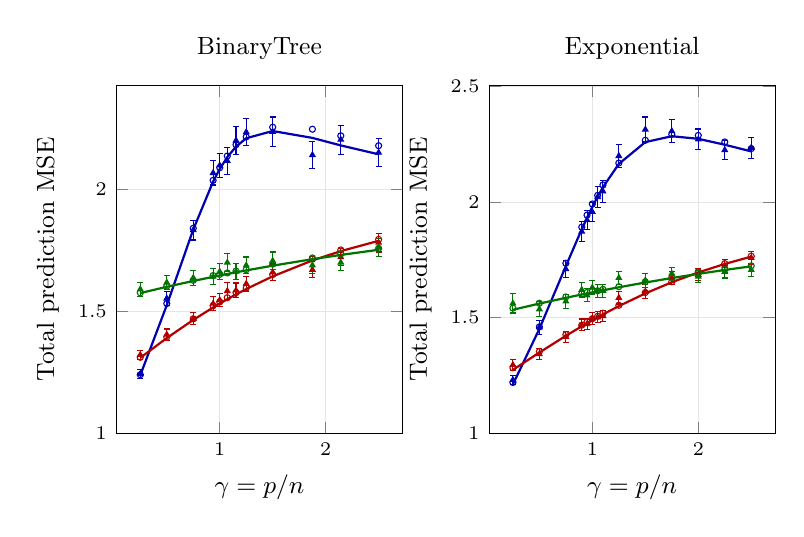
\begin{tikzpicture}
\begin{groupplot}[group style={group size=2 by 1,horizontal sep=1.1cm,vertical sep=1.2cm},
width=.43\linewidth,height=6cm,grid=major,grid style={gray!20},
xlabel={$\gamma=p/n$},ylabel={Total prediction MSE},ymin=1,
tick label style={font=\scriptsize},label style={font=\small},
title style={font=\small}]
\nextgroupplot[title={BinaryTree}]
\addplot[thick,blue!70!black] coordinates {(0.25,1.2379718) (0.5,1.5244323) (0.75,1.8344104) (0.9375,2.030818) (1,2.082157) (1.0714286,2.1308465) (1.1538462,2.1739616) (1.25,2.2081464) (1.5,2.2377491) (1.875,2.2095291) (2.1428571,2.1787493) (2.5,2.1424272)};
\addplot[only marks,mark=o,mark size=1.1pt,blue!70!black] coordinates {(0.25,1.2402021) (0.5,1.5312462) (0.75,1.8396665) (0.9375,2.0357797) (1,2.0875085) (1.0714286,2.1355667) (1.1538462,2.1817003) (1.25,2.2137992) (1.5,2.2533996) (1.875,2.2450909) (2.1428571,2.2181665) (2.5,2.1775928)};
\addplot[only marks,mark=triangle*,mark size=1.1pt,blue!70!black,error bars/.cd,y dir=both,y explicit] coordinates {(0.25,1.2430578) +- (0,0.017542937) (0.5,1.5522467) +- (0,0.029211238) (0.75,1.8321818) +- (0,0.040731345) (0.9375,2.0661669) +- (0,0.049527852) (1,2.0969573) +- (0,0.048535444) (1.0714286,2.115633) +- (0,0.054929377) (1.1538462,2.1989558) +- (0,0.058410438) (1.25,2.2330561) +- (0,0.056383176) (1.5,2.2343227) +- (0,0.060648695) (1.875,2.1397127) +- (0,0.053693424) (2.1428571,2.2025627) +- (0,0.059613319) (2.5,2.1496634) +- (0,0.05768811)};
\addplot[thick,red!70!black] coordinates {(0.25,1.3092983) (0.5,1.3899897) (0.75,1.46432) (0.9375,1.5153075) (1,1.5313549) (1.0714286,1.5491087) (1.1538462,1.5688178) (1.25,1.5907688) (1.5,1.6427254) (1.875,1.7078204) (2.1428571,1.7460398) (2.5,1.7880596)};
\addplot[only marks,mark=o,mark size=1.1pt,red!70!black] coordinates {(0.25,1.3113038) (0.5,1.3938452) (0.75,1.4686881) (0.9375,1.5220609) (1,1.537938) (1.0714286,1.5554107) (1.1538462,1.5759879) (1.25,1.59511) (1.5,1.6499098) (1.875,1.7134816) (2.1428571,1.7508474) (2.5,1.7939803)};
\addplot[only marks,mark=triangle*,mark size=1.1pt,red!70!black,error bars/.cd,y dir=both,y explicit] coordinates {(0.25,1.3213713) +- (0,0.019437219) (0.5,1.4043533) +- (0,0.022593366) (0.75,1.4694232) +- (0,0.024382598) (0.9375,1.5313764) +- (0,0.028382613) (1,1.5458534) +- (0,0.026562064) (1.0714286,1.5830156) +- (0,0.033259355) (1.1538462,1.5852391) +- (0,0.030381466) (1.25,1.6126977) +- (0,0.031028019) (1.5,1.6591203) +- (0,0.034186691) (1.875,1.6697481) +- (0,0.033007482) (2.1428571,1.7215123) +- (0,0.034024791) (2.5,1.7806393) +- (0,0.038322199)};
\addplot[thick,green!45!black] coordinates {(0.25,1.5742533) (0.5,1.5998891) (0.75,1.6238446) (0.9375,1.640756) (1,1.6461991) (1.0714286,1.6523039) (1.1538462,1.6591967) (1.25,1.6670375) (1.5,1.6864474) (1.875,1.7130764) (2.1428571,1.730413) (2.5,1.7515439)};
\addplot[only marks,mark=o,mark size=1.1pt,green!45!black] coordinates {(0.25,1.5755364) (0.5,1.602603) (0.75,1.626469) (0.9375,1.6460388) (1,1.6507998) (1.0714286,1.6567335) (1.1538462,1.6646996) (1.25,1.6699912) (1.5,1.6928003) (1.875,1.7182322) (2.1428571,1.7351118) (2.5,1.7575571)};
\addplot[only marks,mark=triangle*,mark size=1.1pt,green!45!black,error bars/.cd,y dir=both,y explicit] coordinates {(0.25,1.5897424) +- (0,0.027889071) (0.5,1.6175071) +- (0,0.030182956) (0.75,1.6363828) +- (0,0.03108951) (0.9375,1.6418219) +- (0,0.03178391) (1,1.6618192) +- (0,0.032184345) (1.0714286,1.6990607) +- (0,0.037405095) (1.1538462,1.662329) +- (0,0.034217106) (1.25,1.6877442) +- (0,0.034349106) (1.5,1.7063219) +- (0,0.035899842) (1.875,1.6880151) +- (0,0.034646735) (2.1428571,1.6993895) +- (0,0.033279966) (2.5,1.7601578) +- (0,0.036355309)};
\nextgroupplot[title={Exponential}]
\addplot[thick,blue!70!black] coordinates {(0.25,1.2113616) (0.5,1.4519362) (0.75,1.7232631) (0.9,1.8826469) (0.95,1.9323083) (1,1.9794289) (1.05,2.0235898) (1.1,2.0644426) (1.25,2.1649845) (1.5,2.2594372) (1.75,2.284821) (2,2.2735832) (2.25,2.2480123) (2.5,2.2193215)};
\addplot[only marks,mark=o,mark size=1.1pt,blue!70!black] coordinates {(0.25,1.219837) (0.5,1.4603592) (0.75,1.7353813) (0.9,1.8916282) (0.95,1.9437671) (1,1.9916781) (1.05,2.0288984) (1.1,2.0739575) (1.25,2.1686383) (1.5,2.267375) (1.75,2.2927067) (2,2.2883483) (2.25,2.2600263) (2.5,2.2312081)};
\addplot[only marks,mark=triangle*,mark size=1.1pt,blue!70!black,error bars/.cd,y dir=both,y explicit] coordinates {(0.25,1.2309732) +- (0,0.020685372) (0.5,1.4587523) +- (0,0.029798912) (0.75,1.7104163) +- (0,0.037239016) (0.9,1.8725144) +- (0,0.042263928) (0.95,1.9224057) +- (0,0.041423752) (1,1.9574408) +- (0,0.040141127) (1.05,2.0218873) +- (0,0.04572269) (1.1,2.0468077) +- (0,0.047690913) (1.25,2.1995653) +- (0,0.048301295) (1.5,2.3137534) +- (0,0.053988694) (1.75,2.3069175) +- (0,0.048300574) (2,2.2710809) +- (0,0.045106647) (2.25,2.2250652) +- (0,0.041347684) (2.5,2.2352168) +- (0,0.045269636)};
\addplot[thick,red!70!black] coordinates {(0.25,1.2745205) (0.5,1.3494282) (0.75,1.4217862) (0.9,1.4628216) (0.95,1.4760446) (1,1.4890288) (1.05,1.5017691) (1.1,1.5142609) (1.25,1.5502148) (1.5,1.6049794) (1.75,1.6533609) (2,1.6956805) (2.25,1.7324353) (2.5,1.7642084)};
\addplot[only marks,mark=o,mark size=1.1pt,red!70!black] coordinates {(0.25,1.2831744) (0.5,1.3537557) (0.75,1.4272541) (0.9,1.4678216) (0.95,1.4818392) (1,1.4955243) (1.05,1.5061731) (1.1,1.5194972) (1.25,1.5537337) (1.5,1.6089648) (1.75,1.6556734) (2,1.6987399) (2.25,1.7340749) (2.5,1.7660919)};
\addplot[only marks,mark=triangle*,mark size=1.1pt,red!70!black,error bars/.cd,y dir=both,y explicit] coordinates {(0.25,1.2959381) +- (0,0.024527466) (0.5,1.3424793) +- (0,0.02321197) (0.75,1.4174669) +- (0,0.024790868) (0.9,1.4689038) +- (0,0.025412931) (0.95,1.4730483) +- (0,0.02432316) (1,1.4964658) +- (0,0.024922013) (1.05,1.5020499) +- (0,0.023840468) (1.1,1.5076305) +- (0,0.025321818) (1.25,1.5861284) +- (0,0.026978829) (1.5,1.6134846) +- (0,0.029588044) (1.75,1.6725113) +- (0,0.027044462) (2,1.6856825) +- (0,0.02654388) (2.25,1.7243428) +- (0,0.026989158) (2.5,1.7586586) +- (0,0.029239113)};
\addplot[thick,green!45!black] coordinates {(0.25,1.534398) (0.5,1.5610853) (0.75,1.5860636) (0.9,1.6003195) (0.95,1.604953) (1,1.6095279) (1.05,1.6140448) (1.1,1.6185043) (1.25,1.6315426) (1.5,1.652171) (1.75,1.6714809) (2,1.6895427) (2.25,1.7064281) (2.5,1.7222082)};
\addplot[only marks,mark=o,mark size=1.1pt,green!45!black] coordinates {(0.25,1.5411695) (0.5,1.5625113) (0.75,1.5897577) (0.9,1.6032974) (0.95,1.6092695) (1,1.6148148) (1.05,1.6165628) (1.1,1.6224821) (1.25,1.6340581) (1.5,1.655584) (1.75,1.6735353) (2,1.6924958) (2.25,1.7081852) (2.5,1.7242551)};
\addplot[only marks,mark=triangle*,mark size=1.1pt,green!45!black,error bars/.cd,y dir=both,y explicit] coordinates {(0.25,1.5619768) +- (0,0.041711318) (0.5,1.5367545) +- (0,0.03229378) (0.75,1.570833) +- (0,0.030904479) (0.9,1.6210412) +- (0,0.031698432) (0.95,1.5964718) +- (0,0.028024023) (1,1.6302273) +- (0,0.031332681) (1.05,1.6159774) +- (0,0.02686694) (1.1,1.6167608) +- (0,0.028339494) (1.25,1.6720577) +- (0,0.028670175) (1.5,1.6612734) +- (0,0.030268983) (1.75,1.6910046) +- (0,0.02740862) (2,1.6779144) +- (0,0.026815316) (2.25,1.6986919) +- (0,0.026794569) (2.5,1.7067031) +- (0,0.027564161)};
\end{groupplot}\end{tikzpicture}
\caption{两种协方差模型的维数样本比扫描。蓝、红、绿分别对应 $\lambda=0.1,1,4$；实线连接各实际配置下的理论风险，空心圆为条件风险均值，三角及误差线为测试均值及近似点态 $95\%$ 区间。BinaryTree 固定 $p$ 改变 $n$，Exponential 固定 $n$ 改变 $p$；此图为原文实验的扩展。}
\label{fig:covgamma}\end{figure}
\begin{table}[htbp]\centering\small
\caption{两种协方差模型在理论最优点处的总预测风险。}\label{tab:covopt}
\begin{tabular}{lccccc}\toprule
模型 & 实际 $\gamma$ & $\lambda^*$ & 理论 & 条件均值 & 测试均值 $\pm\operatorname{SE}$\\\midrule
BinaryTree & $0.500$ & $0.500$ & $1.3576$ & $1.3603$ & $1.3560\pm0.0111$ \\
BinaryTree & $1.000$ & $1.000$ & $1.5314$ & $1.5397$ & $1.5300\pm0.0141$ \\
BinaryTree & $2.143$ & $2.143$ & $1.7096$ & $1.7185$ & $1.7206\pm0.0186$ \\
Exponential & $0.500$ & $0.500$ & $1.3196$ & $1.3256$ & $1.3263\pm0.0126$ \\
Exponential & $1.000$ & $1.000$ & $1.4890$ & $1.4938$ & $1.5010\pm0.0131$ \\
Exponential & $2.000$ & $2.000$ & $1.6609$ & $1.6637$ & $1.6549\pm0.0144$ \\
\bottomrule\end{tabular}\end{table}
表~\ref{tab:covopt}~给出理论最优点的数值对照。精确条件风险的最优参数仍为 $p/(n\alpha^2)$，协方差结构主要改变风险曲线的水平和形状；测试曲线最低点受有限重复和网格影响。两种谱模型之间的风险差异，应结合整个总体谱以及 $\alpha^2\tr(\Sigma)/p$ 的平均信号方差解释。
对 A1 的判断分为两部分：固定 $\gamma$ 时，以正则路径核对偏差与方差平衡以及理论最优点；固定 $\lambda$ 时，以维数扫描观察插值附近的噪声放大与正则作用。正则为正时风险有限，具体峰值与协方差谱有关，不能把单位协方差图中的形状直接套用到两种模型。
BinaryTree 在本次两类扫描中，测试均值与理论风险的平均绝对差为 $0.0138$，最大绝对差为 $0.2058$。这些差异同时包含有限样本近似误差和模拟误差；误差线仅量化重复均值的不确定性。
Exponential 在本次两类扫描中，测试均值与理论风险的平均绝对差为 $0.0142$，最大绝对差为 $0.1479$。这些差异同时包含有限样本近似误差和模拟误差；误差线仅量化重复均值的不确定性。
一般协方差加权谱公式与直接迹公式的最大差为 $4.26\times10^{-13}$；通用理论在单位协方差下与闭式公式的最大差为 $1.24\times10^{-14}$。相关核验及固定训练特征的模拟检查已随本次本地运行完成。
% END A1 COVARIANCE RESULTS

\begin{thebibliography}{9}
\bibitem{dw}
Dobriban, E., and Wager, S. (2018).
High-dimensional asymptotics of prediction: Ridge regression and classification.
\textit{The Annals of Statistics}, 46(1), 247--279.
DOI: \href{https://doi.org/10.1214/17-AOS1549}{10.1214/17-AOS1549}.
\bibitem{authorcode}
Dobriban, E. \textit{High-dimensional predictive risk: experiment code}.
\href{https://github.com/dobriban/high-dim-risk-experiments}{作者公开实验仓库}，
版本 \filename{d551acd2b3ce283e8ddf3885de4d9fc60dddd766}。
模型及数值方法见 \filename{ridge_hier_sim.m}、\filename{ridge_exp_sim.m}、\filename{compute_ST.m} 和 \filename{simulate_ridge_risk_cov.m}。
\end{thebibliography}
\end{document}
